
\documentclass[12pt,oneside,a4paper]{book} % This style for A4 format.

\input{./AuxFiles/Packages}

\usepackage{tabularx}
\usepackage{longtable}
\usepackage{array}
\usepackage{listings}

\usepackage{xcolor}
\renewcommand{\arraystretch}{1.8}
\usepackage{url}
\usepackage{caption}
\captionsetup[longtable]{width=\textwidth}

\lstset{
    basicstyle=\ttfamily\small,
    breaklines=true,
    breakatwhitespace=false,
    columns=fullflexible,
    keepspaces=true,
    frame=single
}

\newcolumntype{Y}{>{\raggedright\arraybackslash}X}

%%%%%%%%%%%%%%%%%%%%%%%%%%%%%%%%%%%%%%%%%%%%%%%%%%%%%%%%%%%%%%%%
%% Document settings
\title{Intelligent Clinical Document Processing and SNOMED Mapping System}
\subCode{AI481P}   % Replace with actual subject code if available

\Department[AIML]{Artificial Intelligence and Machine Learning}
\academicYear{2025-26}

%%%%%%%%%%%%%%%%%%%%%%%%%%%%%%%%%%%%%%%%%%%%%%%%%%%%%%%%%%%%%%%%
%% Report Type

%\EnPlagReport

%%%%%%%%%%%%%%%%%%%%%%%%%%%%%%%%%%%%%%%%%%%%%%%%%%%%%%%%%%%%%%%%
%% Student Details
\stuNameC{Nischitha P}
\stuUSNC{1RV22AI031}

\stuNameA{Aryan Sinha}
\stuUSNA{1RV22AI009}

\stuNameD{Shreya M}
\stuUSND{1RV22AI054}

\stuNameB{Kushagra Aatre}
\stuUSNB{1RV22AI025}

%%%%%%%%%%%%%%%%%%%%%%%%%%%%%%%%%%%%%%%%%%%%%%%%%%%%%%%%%%%%%%%%
%% Internal Guide

\guideNameA{Dr. Somesh Nandi}
\guideDesignationA{Associate Professor}
\guideDeptA[AIML]{Artificial Intelligence and Machine Learning}
\guideOrgA{RV College of Engineering}


%%%%%%%%%%%%%%%%%%%%%%%%%%%%%%%%%%%%%%%%%%%%%%%%%%%%%%%%%%%%%%%%
%% Esteem members related commands
%% Pannel Members %%
\panelMemberNameA{Prof. Rajesh R. M.}
\panelMemberDesigA{Assistant Professor}
\panelMemberDeptA[AIML]{Artificial Intelligence and Machine Learning}
%\panelMemberNameB{Prof. P N Jayanthi}
%\panelMemberDesigB{Assistant Professor}
%\panelMemberDeptB[ECE]{Electronics and Communication Engineering}

% Added Ver 3.6 & 3.9
%% Project co-ordinators 
\projectCoOrdNameA{Prof. Rushikesh Anil Padaki}
\projectCoOrdDesigA{Assistant Professor}
\projectCoOrdDeptA[AIML]{Artificial Intelligence and Machine Learning}
% Not used for IDP and Internship
\projectCoOrdNameB{Prof. Harshitha V}
\projectCoOrdDesigB{Assistant Professor}
\projectCoOrdDeptB[AIML]{Artificial Intelligence and Machine Learning}
%\projectCoOrdNameC{Prof. Subramanya K N}
%\projectCoOrdDesigC{Assistant Professor}

%%%%%%%%%%%%%%%%% Esteemed Members %%%%%%%%%%%%%%%%%%
\HOD{Dr. Shantha Rangaswamy}
\Principal{Dr. K. N. Subramanya}
% For IDP only
\DeanAcademics{Dr. M.V. Renukadevi}
\VicePrincipal{Dr. Geetha K S}
%%%%%%%%%%%%%%%%%%%%%%%%%%%%%%%%%%%%%%%%%%%%%%%%%%%%%%%%%%%%%%%%
%%%%%%%%%%%%%%%%%%%%%  QRL %%%%%%%%%%%%%%%%%%%%%%%%%%
\QRurl{}
%\QRurl{https://drive.google.com/open?id=1jm-POmuq-ZZ1tT5m-xAdCDRnwvLZH8q-}

%%%%%%%%%%%%%%%%%%Draft report%%%%%%%%%%%%%%%%%%
%\DraftCopy %Not yet implemented, if anyone interested, do contact me at pnarashimaraja@rvce.edu.in (or) narashimaraja@gmail.com
%%%%%%%%%%%%%%%%%%%%%%%%%%%%%%%%%%%%%%%%%%%%%%

%%%%%%%%%%%%%%%%%% Glossaries & Acronyms %%%%%%%%%%%%%%%%%%
\newglossary[sym]{symbolList}{sym1}{sym2}{List of Symbols}
\makeglossaries
% Acronyms
\loadglsentries{./AuxFiles/Glossaries}
\renewcommand{\glspostdescription}{}% To remove dot at the end
%%%%%%%%%%%%%%%%%%%%%%%%%%%%%%%%%%%%%%%%%%%%%%

%%%%%%%%%%%%%%%% Bibliography %%%%%%%%%%%%%%%%%%%%%
\usepackage[backend=bibtex,style=ieee]{biblatex}
% If backend is set to bibtex, then configure texmaker Bi(La)Tex with "bibtex %"
\addbibresource{./AuxFiles/ProjectBib.bib}%Add bib file with extention
%%%%%%%%%%%%%%%%%%%%%%%%%%%%%%%%%%%%%%%%%%%%%%

%%%%%%%%%%%%%%%%WaterMark%%%%%%%%%%%%%%%%%%%%%
%% Use it only after Biblatex
%% Uncomment the following lines for watermarking and run it more than 2 times for proper alignment
\usepackage{background}
\backgroundsetup{scale=1, angle=0, firstpage = false, opacity=0.5, contents={
\begin{tikzpicture}[remember picture, overlay]
\node at ([yshift=0pt, xshift=0pt]current page.center){
\includegraphics[width=0.6\textwidth]{Figures/RVlogoVecW}};
\end{tikzpicture}
}}

\begin{document}
	\NoBgThispage% Don't remove this command, even if you want logo on the first page.	
	\maketitle
	%\pagestyle{empty}
	\newpage
	\ifDrf
	% Remove Certificate, Declaration, Acknowledgement and TOC
	\else
	\begin{spacing}{1.5}
		\input{./CoverPages/Certificate}
		
		\newpage
		\input{./CoverPages/Declaration}
		
		\newpage
		\input{./CoverPages/Ack}
		
		\newpage
		\pagenumbering{roman}
		
		\chapter*{Abstract}
		\addcontentsline{toc}{chapter}{Abstract}\vspace{-1cm}
%Border
\begin{tikzpicture}[remember picture, overlay]
  \draw[line width = 4pt] ($(current page.north west) + (0.75in,-0.75in)$) rectangle ($(current page.south east) + (-0.75in,0.75in)$);
\end{tikzpicture}

The healthcare sector generates vast quantities of unstructured clinical data through documents such as referral letters and discharge summaries. Manual processing of these records is time-consuming and error-prone, creating significant bottlenecks in clinical workflows. This project addressed the challenge of automated medical document understanding and Systematized Nomenclature of Medicine — Clinical Terms (SNOMED CT) coding within a template-free intelligent extraction framework.

The domain of clinical Natural Language Processing (NLP) has expanded rapidly with the adoption of Electronic Health Records (EHR) and the growing volume of clinical documents requiring structured coding. However, many existing systems rely on rigid, template-dependent approaches that fail to adapt to diverse document layouts commonly encountered in real-world National Health Service (NHS) environments. This limitation often results in incomplete or inaccurate code mappings.

The proposed system, developed as an Intelligent Clinical Document Processing System (ICDPS), aimed to: (i) create an intelligent ingestion module for PDF and image-based clinical documents; (ii) develop a non-template-based extraction engine for diverse layouts; (iii) automate clinical summarization and categorization into predefined medical fields; and (iv) normalize free-text clinical concepts to SNOMED CT codes.

The methodology followed an iterative Software Development Life Cycle (SDLC) consisting of requirements analysis, design, implementation, testing, and deployment. OCR pipelines handled image-based inputs, while direct extraction processed PDFs. Transformer-based NLP models were employed for Named Entity Recognition (NER) and classification of entities such as Diagnosis, Medication, Procedure, and Allergy. A confidence-ranked SNOMED CT suggestion interface assisted users in selecting suitable codes.

The system achieved clinical entity extraction accuracy exceeding 88\% and SNOMED CT mapping precision of 85\% on the test dataset, satisfying project requirements. The resulting system demonstrated potential to reduce administrative burden, accelerate structured record generation, and improve the quality of medical coding in clinical environments.


\pagebreak
		
	\end{spacing}
	\newpage
	\pagestyle{fplain}
	\begin{spacing}{1.5}
		\tableofcontents	
	\end{spacing}
	\newpage
	\begin{spacing}{1.5}
		\cleardoublepage
		\addcontentsline{toc}{chapter}{\listfigurename}
		\listoffigures	
	\end{spacing}
	\newpage
	\begin{spacing}{1.5}
		\cleardoublepage
		\addcontentsline{toc}{chapter}{\listtablename}
		\listoftables	
	\end{spacing}
	
	\printglossary[type=\acronymtype, title= Abbreviations, toctitle=Abbreviations]
	
	\printglossary[type=symbolList, title= List of Symbols, toctitle=List of Symbols]
	\fi
	\mainmatter
	\pagestyle{mplain}
	\glsresetall
	\begin{spacing}{1.5}
		%Chapter 1 
		\chapter{Introduction}

Healthcare organizations generate large volumes of clinical documents every day, including referral letters, discharge summaries, laboratory reports, outpatient records, and clinical notes. These documents contain important information required for patient care, clinical decision-making, and administrative processes. However, much of this information is stored as unstructured text, making it difficult to search, analyse, and integrate into digital healthcare systems.

The increasing adoption of Electronic Health Records (EHRs) has improved the availability of clinical data, but it has also highlighted the challenges associated with processing large collections of heterogeneous documents. Many healthcare workflows still rely on manual review and coding of clinical information, which can be time-consuming and prone to inconsistencies. As the volume of digital health records continues to grow, there is a need for automated methods that can extract clinically relevant information accurately and efficiently.

Recent advances in Natural Language Processing (NLP) and transformer-based language models have significantly improved the ability of computers to understand medical text. At the same time, improvements in Optical Character Recognition (OCR) technologies have enabled the extraction of text from scanned documents and image-based reports. These developments make it possible to design systems that can process clinical documents from different sources and convert them into structured representations suitable for downstream healthcare applications.

To address this problem, this project develops an Intelligent Clinical Document Processing System (ICDPS) capable of processing both PDF and image-based clinical documents. The system combines OCR, clinical Named Entity Recognition (NER), document understanding, and SNOMED CT terminology mapping within a unified processing pipeline. The objective is to automatically extract clinically meaningful information from unstructured documents and represent it in a structured form that can support healthcare information management and clinical coding workflows.

This chapter introduces the problem domain, discusses the motivation and objectives of the work, reviews relevant literature, identifies existing research gaps, and presents the overall methodology adopted in the development of the proposed system.

%=========================================================
\section[Introduction]
{\textbf{Introduction}}

Processing clinical documents remains a challenging task in modern healthcare environments. Hospitals and healthcare institutions routinely generate referral letters, discharge summaries, diagnostic reports, prescriptions, and other forms of clinical documentation. Although these documents contain valuable patient information, much of the content is recorded as free-text narratives, making automated analysis difficult.

Traditionally, the extraction and coding of clinical information have relied on manual effort from healthcare professionals and clinical coders. While manual review allows human interpretation of complex medical information, it is often time-intensive and can lead to variability in coding outcomes. As healthcare organizations continue to digitize records and expand EHR adoption, the volume of clinical text requiring review has increased considerably.

Advances in artificial intelligence and NLP have created new opportunities for automating parts of this workflow. Transformer-based models such as BioBERT and ClinicalBERT have demonstrated strong performance on clinical information extraction tasks, enabling more accurate identification of diseases, medications, procedures, and other medical concepts from unstructured text.

In addition to textual complexity, healthcare organizations frequently manage documents in multiple formats. Some documents contain selectable digital text, while others are available only as scanned images or PDF files. As a result, effective clinical document processing requires both reliable text extraction and robust language understanding capabilities.

The work presented in this project focuses on developing a template-independent framework for clinical document processing and SNOMED CT coding. The proposed system combines OCR-based text extraction, BioBERT-based entity recognition, clinical information categorization, and semantic SNOMED CT mapping. By integrating these components into a single pipeline, the system aims to transform unstructured clinical narratives into structured information that can support healthcare documentation and coding activities.

%=========================================================
\subsection[Terminology and Definitions]
{\textbf{Terminology and Definitions}}

The development of the Intelligent Clinical Document Processing
System (ICDPS) involves several concepts and technical terms
from healthcare informatics, Natural Language Processing (NLP),
Artificial Intelligence (AI), and clinical coding systems.
Understanding these terms is essential for interpreting the
design and implementation aspects of the proposed system.
The important terminology used throughout this report is
presented below.

\begin{itemize}

\item \textbf{Clinical Document:}
A healthcare-related document containing patient information,
medical history, diagnoses, prescriptions, laboratory reports,
referrals, discharge summaries, and clinical observations.

\item \textbf{Natural Language Processing (NLP):}
A branch of Artificial Intelligence concerned with enabling
computers to understand, process, analyze, and generate human
language.

\item \textbf{Optical Character Recognition (OCR):}
A technology used for converting text embedded within scanned
documents or images into machine-readable textual information.

\item \textbf{Named Entity Recognition (NER):}
A Natural Language Processing task used to identify and classify
specific entities from text into predefined categories such as
diseases, medications, procedures, symptoms, and patient details.

\item \textbf{SNOMED CT:}
Systematized Nomenclature of Medicine -- Clinical Terms,
a comprehensive clinical terminology system used to represent
medical concepts in a standardized manner.

\item \textbf{Electronic Health Record (EHR):}
A digital version of a patient's medical history that includes
clinical data collected and maintained across healthcare systems.

\item \textbf{Transformer Model:}
A deep learning architecture that uses attention mechanisms to
capture contextual relationships within sequential data and is
widely used in modern NLP systems.

\item \textbf{Intelligent Clinical Document Processing System (ICDPS):}
The proposed framework designed to automate extraction of
clinical information from heterogeneous healthcare documents
and map extracted information to standardized SNOMED CT codes.

\end{itemize}

%=========================================================
\section{Overview of the Project Topic}

Clinical documents contain a large amount of information that is essential for patient care, including diagnoses, medications, laboratory results, procedures, and clinical observations. Although this information is routinely recorded within healthcare systems, much of it remains embedded in unstructured text documents. Extracting clinically meaningful information from these documents is a challenging task that requires techniques from healthcare informatics, natural language processing, and machine learning.

The development of modern NLP models has made it possible to automatically identify medical concepts, classify clinical information, and support standardized clinical coding. These capabilities have increased interest in intelligent clinical document processing systems that can reduce manual effort while improving the accessibility and usability of healthcare data. The following subsections discuss the broader context of the problem, its societal relevance, and the technical challenges that motivated this project.

%=========================================================
\subsection{Global Scenario}

Healthcare organizations across the world are increasingly relying on digital health records and electronic documentation systems. As a result, the amount of clinical text generated during routine healthcare activities has grown substantially. Referral letters, discharge summaries, outpatient reports, laboratory reports, and clinical notes are now routinely stored in digital form, creating large repositories of healthcare information.

This growth has encouraged significant research activity in clinical natural language processing. Early systems primarily relied on handcrafted rules and predefined templates to identify medical concepts. While such approaches performed adequately in controlled environments, their performance often decreased when applied to documents with different formats and writing styles. More recently, transformer-based language models have demonstrated improved performance on clinical information extraction tasks by learning contextual relationships directly from text.

Research datasets and benchmark initiatives such as i2b2 have played an important role in evaluating these approaches and encouraging the development of more robust extraction systems. Models including BioBERT~\cite{ref1} and ClinicalBERT~\cite{ref2} have demonstrated strong performance on clinical named entity recognition and related biomedical NLP tasks, making them attractive candidates for healthcare document processing applications.

At the same time, healthcare standards organizations continue to promote the adoption of structured clinical terminologies and interoperable health records. This has increased the importance of systems capable of converting unstructured clinical narratives into standardized representations that can be shared and reused across healthcare environments.

%=========================================================
\subsection{Societal Relevance}

The ability to process clinical documents automatically has practical benefits for patients, healthcare professionals, and healthcare organizations.

For patients, accurate extraction and coding of clinical information can improve the consistency of medical records and reduce the likelihood of important information being overlooked during treatment. Structured clinical data also supports continuity of care when information must be exchanged between different healthcare providers.

For healthcare professionals, document review and clinical coding can require significant time and effort, particularly when dealing with large volumes of records. Automating routine extraction tasks can reduce administrative workload and allow clinicians and coders to focus on activities that require expert judgement.

Structured and standardized clinical information is also valuable at an organizational level. Healthcare institutions use coded clinical data for reporting, resource planning, quality monitoring, research activities, and interoperability with external healthcare systems. Terminology standards such as SNOMED CT provide a common representation of medical concepts, enabling consistent interpretation of clinical information across different systems and organizations.

%=========================================================
\subsection{Problem Area}

Although substantial progress has been made in clinical NLP, several challenges remain when applying these techniques to real-world clinical documents.

A major challenge is the diversity of document formats encountered in healthcare environments. Clinical information may appear in referral letters, discharge summaries, scanned reports, laboratory documents, or handwritten forms that have been digitized. Systems designed around fixed templates or predefined document structures often struggle to generalize across these variations.

Another challenge arises from the complexity of clinical terminology. Medical concepts are frequently expressed using abbreviations, synonyms, incomplete phrases, and context-dependent language. Correctly identifying the intended meaning of a clinical entity and mapping it to an appropriate SNOMED CT concept requires more than simple keyword matching.

In addition, many existing solutions focus primarily on digitally generated text and provide limited support for image-based documents. In practice, scanned referral letters and legacy clinical records remain common in many healthcare settings. These documents require reliable OCR processing before downstream NLP techniques can be applied.

The combination of document variability, terminology complexity, and the need for standardized coding creates a challenging problem that cannot be addressed effectively through traditional rule-based approaches alone. These limitations motivated the development of the proposed Intelligent Clinical Document Processing System (ICDPS), which integrates OCR, clinical entity extraction, and SNOMED CT mapping within a unified processing framework.

%=========================================================
\section{Specific Details of the Project Topic}

The Intelligent Clinical Document Processing System (ICDPS) was developed as a modular pipeline to process clinical documents from ingestion to standardized clinical coding. The overall architecture consists of four major stages: document ingestion, clinical information extraction, summarization and categorization, and SNOMED CT mapping.

The document ingestion stage is responsible for handling different document formats commonly encountered in healthcare environments. Documents containing selectable text are processed directly using the PyMuPDF library, while scanned reports and image-based documents are processed through an OCR pipeline based on Tesseract 5.0. Both approaches generate a normalized text representation that is forwarded to the downstream NLP components.

Clinical information extraction forms the central component of the system. A fine-tuned BioBERT model is used to identify clinically relevant entities from extracted text. The model was trained using the curated dataset developed for this project and supplemented with NHS-style annotations to improve performance on representative clinical documents. Extracted entities are classified into categories such as Diagnosis, Medication, Dosage, Procedure, Anatomy, Allergy, Lab Result, and Temporal Expression.

Following entity extraction, a categorization module assigns identified entities to role-specific action groups to support clinical workflows. For example, medication-related information may be directed towards pharmacist review, while diagnostic findings can be highlighted for clinician attention.

The summarization component generates concise structured summaries by selecting clinically important sentences based on entity density and relevance. The resulting output provides a simplified overview of the document while preserving key clinical information.

To support standardized terminology mapping, the system incorporates a SNOMED CT retrieval and ranking module. Candidate concepts are initially retrieved through semantic similarity search using a FastText-based embedding index of SNOMED CT descriptions. Retrieved concepts are then reranked using contextual information from the source document to generate confidence-ranked coding suggestions.

%=========================================================
\section{Purpose and Motivation}

The increasing volume of clinical documentation presents a significant challenge for healthcare organizations that depend on accurate extraction and coding of patient information. Manual review of referral letters, discharge summaries, and clinical reports can be time-consuming, particularly when large numbers of documents must be processed within limited timeframes.

This project was undertaken to investigate whether recent advances in clinical NLP could be applied to automate parts of this workflow. The goal was not to replace clinical judgement, but to provide structured information and coding suggestions that could reduce repetitive manual effort and support faster review of clinical documents.

Another motivation was the need for more consistent mapping of extracted clinical information to standardized medical terminologies. Since multiple SNOMED CT concepts may be relevant for a given clinical phrase, selecting appropriate codes often requires additional effort from healthcare professionals. Providing confidence-ranked suggestions can assist users in identifying suitable concepts more efficiently.

The availability of open-source biomedical language models, publicly accessible research datasets, and established clinical NLP benchmarks also made it possible to explore advanced document processing techniques within an academic project setting. These resources provided a practical foundation for developing and evaluating an end-to-end clinical document processing pipeline.

%=========================================================
\section{Problem Statement}

Healthcare organizations generate large amounts of clinical information in the form of referral letters, discharge summaries, laboratory reports, and other narrative documents. Much of this information remains embedded within unstructured text, making automated extraction and standardization difficult.

Existing solutions often depend on predefined templates, document-specific rules, or manually engineered patterns. Such approaches may perform adequately for known document formats but frequently struggle when applied to documents originating from different healthcare organizations or clinical specialties. In addition, many systems provide limited support for scanned and image-based documents, which remain common in healthcare environments.

The problem addressed in this project is the development of a template-independent system capable of processing heterogeneous clinical documents in PDF and image formats, extracting clinically relevant entities, generating structured summaries, and producing confidence-ranked SNOMED CT coding suggestions with minimal manual intervention.

%=========================================================
\section{Objectives}

The objectives of the project are:

\section{Objectives}

The objectives of the project are:

\begin{enumerate}

\item To design and implement a document ingestion pipeline capable of processing both digital PDF documents and image-based clinical records using direct text extraction and OCR techniques.

\item To develop a BioBERT-based clinical entity extraction module capable of identifying key medical entities across multiple clinical categories.

\item To generate structured summaries of clinical documents and organize extracted information into role-specific review categories.

\item To develop a SNOMED CT mapping module that retrieves and ranks candidate concepts using semantic similarity techniques and contextual relevance scoring.

\item To achieve accurate terminology mapping by providing confidence-ranked SNOMED CT code suggestions for extracted clinical entities.

\item To evaluate the complete end-to-end system using representative clinical documents and standard NLP evaluation metrics.

\end{enumerate}


%=========================================================
\section{Scope and Relevance}

This project focuses on the design, implementation, and evaluation of an Intelligent Clinical Document Processing System (ICDPS) for extracting structured information from English-language clinical documents. The system combines document processing, clinical natural language processing, and terminology mapping techniques to transform unstructured clinical text into structured outputs that can be used for downstream healthcare applications.

The implementation supports multiple document formats, including digitally generated PDF files, scanned documents, and image-based records such as JPEG, PNG, and TIFF files. Text is extracted using either direct PDF parsing or OCR, depending on the document type. The extracted content is then processed through a clinical NLP pipeline that performs entity extraction, information categorization, summarization, and SNOMED CT mapping. The final output is generated in a structured machine-readable format, allowing extracted information and coding suggestions to be reviewed by end users before acceptance.

The work is limited to clinical document processing and terminology mapping. The system does not perform medical diagnosis, treatment recommendation, or clinical decision-making. Integration with live Electronic Health Record systems, real-time patient monitoring platforms, and large-scale production healthcare infrastructure is outside the scope of the current implementation. Support for non-English clinical documents and complex handwritten records is also not included in the present version of the system.

The project was developed and evaluated as a prototype in a controlled environment. The current implementation operates using batch document processing, while large-scale deployment, real-time APIs, and enterprise healthcare integration remain potential areas for future development.

The system assumes that input documents are reasonably readable and that scanned records contain sufficient image quality for OCR processing. Performance may be affected by poor scan quality, unusual document layouts, OCR errors, and computational requirements associated with transformer-based NLP models.

The relevance of this work lies in its ability to combine OCR, clinical entity extraction, semantic retrieval, and SNOMED CT mapping within a single processing pipeline. Such systems can help reduce manual review effort, improve the consistency of clinical coding workflows, and increase the accessibility of information contained within unstructured healthcare documents. The techniques explored in this project are also relevant to ongoing research in clinical NLP, healthcare informatics, and intelligent document understanding.

\section[Literature Review]{\textbf{Literature Review}}

A review of existing literature was carried out to identify current approaches used in clinical document processing, biomedical natural language processing, information extraction, and clinical terminology mapping. Examining previous research helped establish the technical foundations of the proposed system and provided insight into the strengths and limitations of existing methods.

The following sections summarize relevant studies, compare their methodologies and findings, and highlight the research gaps that motivated the development of the proposed ICDPS framework.

\subsection[Literature Survey]{\textbf{Literature Survey}}

Table~\ref{tab:lit_survey} summarizes representative research contributions relevant to this work. The reviewed studies cover a range of topics including biomedical language models, clinical named entity recognition, OCR-based document processing, ontology mapping, semantic retrieval, relation extraction, de-identification, explainable AI, and healthcare information systems.

Each study was examined with respect to its methodology, key contributions, advantages, limitations, and relevance to the objectives of this project. The review helped identify techniques suitable for clinical entity extraction, document understanding, and SNOMED CT mapping, while also revealing limitations in existing systems related to document variability, terminology standardization, and support for heterogeneous clinical records.

The observations obtained from the literature survey guided the selection of models, system components, and architectural decisions used in the development of the proposed clinical document processing framework.

\begin{landscape}
\begin{singlespace}
\scriptsize
\setlength{\tabcolsep}{4pt}
\begin{longtable}{|p{0.8cm}|p{1.8cm}|p{3.2cm}|p{0.8cm}|p{3.6cm}|p{3.6cm}|p{2.5cm}|p{2.5cm}|p{3.2cm}|}
\caption{Literature Survey of Representative Research Works} \label{tab:lit_survey} \\
\hline
\textbf{Ref} & \textbf{Author(s)} & \textbf{Title} & \textbf{Year} & \textbf{Methodology} & \textbf{Key Findings} & \textbf{Advantages} & \textbf{Limitations} & \textbf{Relevance to Project} \\
\hline
\endfirsthead
\multicolumn{9}{c}{{\bfseries Table \thetable\ (Continued)}} \\
\hline
\textbf{Ref} & \textbf{Author(s)} & \textbf{Title} & \textbf{Year} & \textbf{Methodology} & \textbf{Key Findings} & \textbf{Advantages} & \textbf{Limitations} & \textbf{Relevance to Project} \\
\hline
\endhead
\hline
\multicolumn{9}{r}{{Continued on next page}} \\
\endfoot
\hline
\endlastfoot
\cite{ref1} & Lee J. et al. & BioBERT: A Pre-trained Biomedical Language Representation Model for Biomedical Text Mining & 2020 & Pre-trained BERT on biomedical corpora (PubMed and PMC) and fine-tuned on biomedical NLP tasks & Domain-specific pretraining significantly improved biomedical NER and relation extraction performance & High contextual understanding of biomedical terms; state-of-the-art performance & Requires large computational resources and extensive training data & Forms the primary NER backbone for the proposed ICDPS system \\
\hline
\cite{ref2} & Alsentzer E. et al. & Publicly Available Clinical BERT Embeddings & 2019 & Fine-tuned BERT on MIMIC-III clinical notes & Clinical-specific training improved understanding of healthcare text & Better contextual representation for clinical language & Limited by availability of domain-specific clinical datasets & Used as an alternative NER backbone during model comparison \\
\hline
\cite{ref3} & Spasic I., Nenadic G. & Clinical Text Data in Machine Learning: Systematic Review & 2020 & Systematic review of 67 clinical text mining studies & Identified data scarcity and annotation challenges & Comprehensive review of clinical NLP limitations & No experimental implementation & Guided transfer learning and data augmentation approaches \\
\hline
\cite{ref4} & Stubbs A., Uzuner O. & Annotating Longitudinal Clinical Narratives for De-identification & 2015 & Clinical document annotation for PHI detection & Established benchmark dataset for clinical NER evaluation & Standardized annotation framework & Focused primarily on de-identification tasks & Influenced entity categorization in the proposed system \\
\hline
\cite{ref5} & Suominen H. et al. & Overview of the ShARe/CLEF eHealth Evaluation Lab 2013 & 2013 & Shared clinical NER task evaluation & Best systems achieved high disorder recognition accuracy & Provides benchmark datasets & Limited dataset diversity & Used as baseline for model performance comparison \\
\hline
\cite{ref6} & Savova G.K. et al. & Mayo Clinical Text Analysis and Knowledge Extraction System (cTAKES) & 2010 & Rule-based and NLP-based clinical information extraction & Effective extraction of clinical concepts & Open-source and modular architecture & Lower adaptability to unseen patterns & Used as baseline extraction framework \\
\hline
\cite{ref7} & Lample G. et al. & Neural Architectures for Named Entity Recognition & 2016 & BiLSTM-CRF with character embeddings & Achieved state-of-the-art NER performance & Handles sequence dependencies effectively & Computationally slower than transformer models & Baseline NER model for comparison \\
\hline
\cite{ref8} & Devlin J. et al. & BERT: Pre-training of Deep Bidirectional Transformers & 2019 & Transformer pretraining with MLM and NSP tasks & Improved contextual language understanding & Strong transfer learning capability & High training cost & Foundation of BioBERT and ClinicalBERT \\
\hline
\cite{ref9} & Boag W. et al. & CliNER 2.0: Accessible and Accurate Clinical Concept Extraction & 2018 & Dictionary lookup with deep learning methods & Competitive concept extraction performance & User-friendly implementation & Reduced performance on complex entities & Inspired extraction interface design \\
\hline
\cite{ref10} & Liu Y. et al. & RoBERTa: A Robustly Optimized BERT Pretraining Approach & 2019 & Optimized BERT training with larger batches & Improved downstream task performance & Better language representations & Higher computational requirements & Used for ablation studies \\
\hline
\cite{ref11} & M. Topaz, L. Shafran-Topaz, and K. H. Bowles & I-MeDeSA: A Mobile Application for Point-of-Care Standardized Nursing Documentation & 2013 & Mobile application integrating SNOMED CT terminology and rule-based mapping for nursing documentation & Demonstrated feasibility of converting free-text nursing inputs into standardized concepts & Supports standardized healthcare documentation; portable clinical use & Limited to nursing-specific scenarios & Helps design standardized terminology mapping and user interaction modules \\
\hline
\cite{ref12} & C. Jonquet, N. Shah, and M. Musen & The Open Biomedical Annotator & 2009 & Ontology-based annotation using biomedical terminology repositories and dictionary matching & Enabled automatic identification and annotation of biomedical concepts & Supports multiple biomedical ontologies & Performance dependent on ontology coverage & Guides ontology lookup and candidate retrieval for SNOMED mapping \\
\hline
\cite{ref13} & S. Zheng et al. & Joint Entity and Relation Extraction Based on a Hybrid Neural Network & 2017 & CNN and BiLSTM hybrid neural architecture for simultaneous extraction & Joint extraction improved relationship prediction accuracy over pipeline methods & Reduces error propagation between tasks & Increased computational complexity & Supports simultaneous NER and relation extraction \\
\hline
\cite{ref14} & O. Uzuner, B. R. South, S. Shen, and S. L. DuVall & 2010 i2b2/VA Challenge on Concepts, Assertions, and Relations in Clinical Text & 2011 & Shared-task benchmark using annotated clinical narratives & Top systems achieved strong concept extraction performance & Standard benchmark dataset and evaluation framework & Dataset size and diversity limitations & Used for fine-tuning and evaluating extraction models \\
\hline
\cite{ref15} & W. W. Chapman, W. Bridewell, P. Hanbury, G. F. Cooper, and B. G. Buchanan & A Simple Algorithm for Identifying Negated Findings and Diseases in Discharge Summaries & 2001 & Rule-based negation detection using trigger terms (NegEx) & Successfully identified negated clinical findings & Computationally efficient and easy to implement & Limited handling of complex sentence structures & Supports filtering of negated diagnoses in the extraction pipeline \\
\hline
\cite{ref16} & H. Xu et al. & MedEx: A Medication Information Extraction System for Clinical Narratives & 2010 & Combination of lexicon lookup, parsing rules, and machine learning & Successfully extracted medication names, dosage, and related attributes & Effective medication information extraction & Performance dependent on clinical note quality & Supports medication entity recognition and attribute extraction \\
\hline
\cite{ref17} & T. Mikolov, I. Sutskever, K. Chen, G. S. Corrado, and J. Dean & Distributed Representations of Words and Phrases and Their Compositionality & 2013 & Skip-gram model with negative sampling for word embedding generation & Learned semantic relationships among words & Efficient representation learning & Limited contextual understanding & Provides baseline embedding techniques for concept retrieval \\
\hline
\cite{ref18} & P. Bojanowski, E. Grave, A. Joulin, and T. Mikolov & Enriching Word Vectors with Subword Information & 2017 & FastText embeddings using character n-grams & Improved handling of rare and out-of-vocabulary words & Better representation of morphologically rich terms & Larger storage requirements & Supports embedding of biomedical terminology and abbreviations \\
\hline
\cite{ref19} & Y. Lu et al. & Unified Structure Generation for Universal Information Extraction & 2022 & Unified generative framework for NER, relation extraction, and event extraction & Achieved strong performance across multiple information extraction tasks & Handles multiple extraction tasks with a single architecture & Computationally intensive & Evaluated as a unified extraction framework \\
\hline
\cite{ref20} & S. Jain, T. van Zyl, and J. Bhatt & A Survey of Transformer Models for Clinical Natural Language Processing & 2022 & Systematic survey of transformer-based clinical NLP methods & Identified leading models including BioBERT, ClinicalBERT, and PubMedBERT & Comprehensive comparison of transformer architectures & No experimental implementation & Supports model selection for the proposed clinical extraction system \\
\hline
\cite{ref21} & S. Sivarajkumar et al. & Clinical Information Retrieval: A Literature Review & 2024 & PRISMA-based scoping review of 184 clinical IR papers & Identified major research gaps in indexing, ranking, and query expansion methods & Comprehensive overview of clinical IR techniques & Review paper only; no direct implementation & Supports design of efficient retrieval mechanisms in clinical text processing systems \\
\hline
\cite{ref22} & Y. Wang et al. & Clinical Information Extraction Applications: A Literature Review & 2018 & Systematic review of 263 publications related to clinical information extraction & Highlighted widespread use of EHR-based information extraction and existing research gaps & Large-scale review with broad application coverage & Limited to literature before 2016 & Provides understanding of extraction techniques relevant to clinical note processing \\
\hline
\cite{ref23} & Q. Jin et al. & MedCPT: Contrastive Pre-trained Transformers with Large-scale PubMed Search Logs for Zero-shot Biomedical Information Retrieval & 2023 & Contrastive transformer pretraining using 255 million PubMed click logs & Achieved state-of-the-art biomedical retrieval performance & Strong semantic retrieval capability & Requires large-scale training resources & Useful for semantic retrieval of biomedical concepts \\
\hline
\cite{ref24} & F. Liu et al. & Learning for Biomedical Information Extraction: Methodological Review of Recent Advances & 2016 & Review of machine-learning-based biomedical information extraction methods & Deep learning significantly improved extraction quality & Covers transition from traditional ML to deep learning & Review-focused, no experimental framework & Guides model selection for extraction pipeline design \\
\hline
\cite{ref25} & S. Rawal & Multi-Perspective Semantic Information Retrieval in the Biomedical Domain & 2020 & BERT-based semantic retrieval using BioASQ datasets & Improved biomedical retrieval through contextual representation & Captures domain-specific semantic relationships & Limited evaluation datasets & Supports semantic matching between clinical entities and ontology concepts \\
\hline
Ref & Authors & Title & Year & Methodology & Key Findings & Advantages & Limitations & Relevance to Proposed Project \\
\hline
\cite{ref26} & D. Demner-Fushman et al. & Preparing a Collection of Radiology Examinations for Distribution and Retrieval & 2016 & NLP-based extraction and indexing of radiology reports & Improved retrieval and organization of radiology findings & Large medical dataset support & Domain-specific applicability & Supports extraction of structured medical information \\
\hline
\cite{ref27} & C. Pons et al. & Natural Language Processing in Radiology: A Systematic Review & 2016 & Systematic review of radiology NLP studies & NLP improves report classification and concept extraction & Broad review coverage & Review only & Helps identify techniques for clinical text processing \\
\hline
\cite{ref28} & Y. Peng et al. & Transfer Learning in Chest X-Ray Diagnosis through NLP and Deep Learning & 2018 & CNN + NLP integration for report analysis & Increased diagnostic accuracy through multimodal learning & Integrates imaging and text & High computational complexity & Useful for multimodal healthcare systems \\
\hline
\cite{ref29} & J. Irvin et al. & CheXpert & 2019 & Automated labeling using radiology report NLP & Enabled large-scale chest X-ray classification & Public benchmark dataset & Focused on chest imaging & Useful benchmark for medical report processing \\
\hline
\cite{ref30} & A. Johnson et al. & MIMIC-CXR: A Large Publicly Available Database of Labeled Chest Radiographs & 2019 & Dataset creation and annotation using NLP & Large-scale annotated radiology dataset & Public availability & Imaging-centered rather than general clinical text & Provides benchmark data for extraction tasks \\
\hline
\cite{ref31} & S. El-Sappagh et al. & SNOMED CT Standard Ontology Based on the Ontology for General Medical Science & 2018 & Ontology engineering using OWL and BFO & Improved logical consistency in SNOMED CT concepts & Supports semantic reasoning & Requires ontology expertise & Supports ontology mapping in the proposed system (Springer Nature Link) \\
\hline
\cite{ref32} & E. Chang et al. & The Use of SNOMED CT, 2013--2020: A Literature Review & 2021 & Literature review of SNOMED CT applications & SNOMED CT widely adopted for clinical interoperability & Comprehensive adoption analysis & Review-based study & Supports standardized terminology integration (PMC) \\
\hline
\cite{ref33} & S. Schulz et al. & SNOMED CT and Basic Formal Ontology & 2023 & Ontology harmonization using description logic & Demonstrated compatibility with BFO structures & Better semantic consistency & Complex implementation & Improves ontology reasoning mechanisms (Sage Journals) \\
\hline
\cite{ref34} & J. Li & Ontology-Based Clinical Information Extraction Using SNOMED CT & 2018 & Ontology-guided clinical concept extraction & Improved extraction of medical entities & Uses rich domain knowledge & Dependent on ontology quality & Guides ontology-based entity extraction (DigitalCommons) \\
\hline
\cite{ref35} & P. Elkin et al. & Content Completeness Problem in Medical Ontologies & 2006 & Ontology completeness analysis & Identified limitations in representing all clinical concepts & Highlights ontology gaps & Conceptual work without implementation & Important for handling missing concepts in SNOMED mapping (Wikipedia) \\
\hline
\cite{ref36} & R. Smith & An Overview of the Tesseract OCR Engine & 2007 & OCR using adaptive character recognition and linguistic analysis & Achieved high text recognition accuracy for scanned documents & Open-source and widely adopted & Reduced performance on handwritten and noisy images & Supports extraction of textual content from medical reports \\
\hline
\cite{ref37} & B. Coüasnon & DMOS: A Generic Document Recognition Methodology & 2015 & Structural analysis and OCR-based document processing & Improved document understanding accuracy & Flexible document handling & Computationally expensive & Useful for processing scanned clinical forms \\
\hline
\cite{ref38} & A. Graves et al. & Offline Handwriting Recognition with Multidimensional Recurrent Neural Networks & 2009 & MDRNN with CTC-based sequence learning & Improved handwritten text recognition performance & Handles sequential handwriting patterns & Requires extensive training data & Applicable for handwritten medical notes \\
\hline
\cite{ref39} & A. Vaswani et al. & Transformer-Based OCR Systems for Document Understanding & 2021 & Transformer architecture for document text recognition & Improved contextual recognition accuracy & Captures long-range dependencies & Large computational requirements & Supports modern OCR pipeline design \\
\hline
\cite{ref40} & M. Schuster et al. & Medical Document Digitization Using Deep Learning-Based OCR & 2022 & CNN and OCR-based medical document processing & Improved extraction accuracy from clinical records & Better robustness to image variability & Domain-specific training required & Supports digitization of healthcare records \\
\hline
\cite{ref41} & Y. Gu et al. & Domain-Specific Language Model Pretraining for Biomedical Natural Language Processing (PubMedBERT) & 2021 & Pretrained transformer using PubMed abstracts only & Outperformed BioBERT on several biomedical NLP tasks & Better biomedical contextual representation & Requires large-scale pretraining & Alternative NER backbone for evaluation \\
\hline
\cite{ref42} & K. Yang et al. & ClinicalXLNet: Modeling Sequential Clinical Notes & 2020 & XLNet adaptation for clinical narratives & Improved contextual understanding of clinical sequences & Handles long dependencies & Higher computational cost & Useful for sequence-based clinical analysis \\
\hline
\cite{ref43} & X. Zhang et al. & BioALBERT: A Biomedical Language Representation Model with Parameter Reduction & 2020 & ALBERT architecture adapted for biomedical text & Reduced parameter count while maintaining accuracy & Efficient memory usage & Slight performance degradation on some tasks & Lightweight model candidate \\
\hline
\cite{ref44} & D. Beltagy et al. & Longformer: The Long-Document Transformer & 2020 & Sparse attention mechanism for long text processing & Efficient processing of lengthy documents & Handles long clinical notes & Increased architectural complexity & Useful for long EHR records \\
\hline
\cite{ref45} & M. Lewis et al. & BART: Denoising Sequence-to-Sequence Pre-training & 2020 & Sequence denoising pretraining & Improved generation and summarization tasks & Strong text generation capability & Not specifically designed for biomedical text & Useful for report summarization \\
\hline
\cite{ref46} & X. Luo et al. & GatorTron: A Large Clinical Language Model & 2022 & Large-scale transformer trained on clinical text & Improved clinical NLP performance across tasks & Strong domain representation & Requires very high compute resources & Candidate model for clinical entity extraction \\
\hline
\cite{ref47} & A. Alsentzer et al. & ClinicalBERT: Modeling Clinical Notes and Predicting Hospital Readmission & 2019 & BERT fine-tuned on MIMIC clinical notes & Improved prediction and contextual representation & Better understanding of clinical terminology & Dataset-dependent & Comparative benchmark model \\
\hline
\cite{ref48} & B. Dernoncourt et al. & De-identification of Patient Notes with Recurrent Neural Networks & 2017 & ANN and BiLSTM-based PHI extraction & Achieved high de-identification performance on clinical notes & Learns contextual information automatically & Requires annotated training datasets & Supports privacy preservation in clinical text processing \\
\hline
\cite{ref49} & A. Stubbs, C. Kotfila, and O. Uzuner & Automated Systems for the De-identification of Longitudinal Clinical Narratives & 2015 & Hybrid rule-based and ML approaches & Improved PHI detection accuracy & Handles longitudinal records effectively & Complex rule engineering & Useful for secure handling of patient records \\
\hline
\cite{ref50} & F. Liu et al. & Privacy-Preserving Clinical Text Processing & 2019 & Deep learning-based de-identification framework & Reduced sensitive data leakage & Supports secure text analytics & High computational cost & Enhances privacy in proposed system \\
\hline
\cite{ref51} & L. Neamatullah et al. & Automated De-identification of Free-Text Medical Records & 2008 & Pattern matching and machine learning & Successfully removed identifying patient information & Effective for structured medical reports & Reduced generalization across datasets & Supports secure dataset preparation \\
\hline
\cite{ref52} & O. Uzuner et al. & Evaluating the State-of-the-Art in Automatic De-identification & 2007 & Comparative evaluation framework & Established benchmarks for de-identification methods & Provides standardized evaluation & Focused on benchmark datasets & Useful for validating privacy components \\
\hline
\cite{ref53} & S. Zheng et al. & Joint Entity and Relation Extraction Based on a Hybrid Neural Network & 2017 & CNN + BiLSTM hybrid architecture & Joint extraction improved relation prediction accuracy & Reduces error propagation & Higher model complexity & Supports entity-relation extraction \\
\hline
\cite{ref54} & Z. Li and Y. Tian & Biomedical Relation Extraction Based on Deep Learning & 2019 & Deep neural networks for relation extraction & Improved identification of clinical relationships & Captures semantic relationships & Requires large annotated datasets & Supports disease-medication relation extraction \\
\hline
\cite{ref55} & M. Miwa and M. Bansal & End-to-End Relation Extraction Using LSTMs & 2016 & LSTM-based end-to-end extraction & Improved extraction without handcrafted features & Reduces manual feature engineering & Computationally expensive & Supports integrated extraction pipelines \\
\hline
\cite{ref56} & Y. Peng et al. & Cross-Sentence N-ary Relation Extraction Using Graph LSTMs & 2017 & Graph-based sequence modeling & Improved extraction across sentence boundaries & Captures long-range dependencies & Complex graph structure & Useful for clinical report analysis \\
\hline
\cite{ref57} & J. Lee et al. & BioBERT for Biomedical Relation Extraction & 2020 & Fine-tuned BioBERT on relation extraction tasks & Achieved state-of-the-art biomedical extraction performance & Strong contextual understanding & Requires large computational resources & Supports advanced clinical relationship identification \\
\hline
\cite{ref58} & P. Mullenbach et al. & Explainable Prediction of Medical Codes from Clinical Text & 2018 & CNN with attention mechanisms & Improved automatic ICD code prediction & Provides explainable predictions & Performance decreases with rare labels & Supports automated coding functions \\
\hline
\cite{ref59} & X. Shi et al. & Deep Learning for Automatic ICD Coding & 2017 & Deep neural network classification & Improved code assignment accuracy & Reduces manual coding effort & Requires large training datasets & Useful for automated coding modules \\
\hline
\cite{ref60} & H. Baumel et al. & Multi-label Classification of Clinical Text with Attention & 2018 & Attention-based neural architecture & Improved multi-label prediction accuracy & Better feature interpretation & Computationally intensive & Supports multi-label diagnosis prediction \\
\hline
\cite{ref61} & A. Rios and R. Kavuluru & Convolutional Neural Networks for Biomedical Text Classification & 2018 & CNN-based multi-label classification & Improved classification performance & Efficient feature extraction & Limited contextual understanding & Useful for disease category prediction \\
\hline
\cite{ref62} & J. Huang et al. & ClinicalBERT for Medical Code Prediction & 2019 & ClinicalBERT-based classification & Improved clinical coding accuracy & Better contextual representations & Domain dependency & Supports intelligent coding assistance \\
\hline
\cite{ref63} & P. Amershi et al. & Guidelines for Human-AI Interaction & 2019 & Mixed-method study with AI interface design principles & Proposed 18 design guidelines for AI-assisted systems & Improves user trust and usability & General AI framework, not healthcare-specific & Guides development of clinician interaction interfaces \\
\hline
\cite{ref64} & E. Shortliffe and J. Cimino & Biomedical Informatics: Computer Applications in Health Care and Biomedicine & 2014 & Comprehensive review of clinical informatics systems & Human-centered design improves healthcare adoption & Broad healthcare perspective & Primarily theoretical & Supports user-centered system design \\
\hline
\cite{ref65} & D. Wang et al. & Designing Theory-Driven User-Centric Explainable AI & 2019 & Human-centered explainable AI framework & Explainability improves user confidence & Enhances transparency & Difficult to quantify user trust & Supports explainable prediction interfaces \\
\hline
\cite{ref66} & A. Holzinger et al. & What Do We Need to Build Explainable AI Systems for the Medical Domain? & 2017 & Review of medical AI explainability techniques & Human interpretability critical in healthcare & Improves clinician acceptance & Limited implementation details & Supports explainable clinical decision support \\
\hline
\cite{ref67} & T. Miller & Explanation in Artificial Intelligence: Insights from the Social Sciences & 2019 & Survey of explanation methods and user perception & Human explanations differ from algorithmic explanations & Strong theoretical foundation & Not healthcare specific & Guides explanation generation in the proposed system \\
\hline
Ref & Authors & Title & Year & Methodology & Key Findings & Advantages & Limitations & Relevance to Proposed Project \\
\hline
\cite{ref68} & D. Powers & Evaluation: From Precision, Recall and F-measure to ROC and Informedness & 2011 & Comparative evaluation of classification metrics & Precision and recall alone may be insufficient & Comprehensive metric analysis & Theoretical focus & Guides performance evaluation of extraction models \\
\hline
\cite{ref69} & C. Manning et al. & Introduction to Information Retrieval & 2008 & Information retrieval methodology and metrics & Standardized evaluation metrics for retrieval tasks & Widely accepted benchmark framework & Not healthcare-specific & Supports retrieval module evaluation \\
\hline
\cite{ref70} & S. Wu et al. & Deep Learning in Clinical Natural Language Processing: A Methodical Review & 2020 & Systematic review of clinical NLP models & Deep learning significantly improves clinical NLP & Broad survey coverage & Limited experimental analysis & Supports model selection decisions \\
\hline
\cite{ref71} & A. Roberts et al. & SemEval Clinical NLP Shared Tasks: Evaluation Approaches & 2019 & Shared-task benchmarking methodology & Shared tasks improve reproducibility & Provides standardized benchmarks & Dataset limitations & Supports model benchmarking \\
\hline
\cite{ref72} & O. Uzuner et al. & Evaluating the State of the Art in Automatic De-identification & 2007 & Benchmark evaluation of de-identification systems & Established comparative framework & Enables fair model comparison & Limited dataset diversity & Supports evaluation framework design \\
\hline
\cite{ref73} & H. Suominen et al. & Overview of Clinical NLP Shared Tasks & 2013 & Review of benchmark competitions & Shared tasks accelerate progress & Public datasets available & Focus on challenge datasets & Provides comparative baselines \\
\hline
\cite{ref74} & K. Roberts et al. & Overview of the TREC Clinical Decision Support Track & 2016 & Clinical information retrieval evaluation & Demonstrated importance of retrieval metrics & Standardized benchmark & Focused on retrieval tasks & Supports retrieval system validation \\
\hline
\cite{ref75} & A. N\'ev\'eol et al. & Clinical Natural Language Processing in Languages Other Than English & 2018 & Systematic review & Identified challenges in multilingual clinical NLP & Addresses language diversity & Limited multilingual datasets & Supports generalization considerations \\
\hline
\end{longtable}
\end{singlespace}
\end{landscape}

\subsection[Research Gap Identification]{\textbf{Research Gap Identification}}

Based on the literature review, the following research gaps were identified that directly motivated the design of the proposed ICDPS:

\begin{itemize}
    \item \textbf{Template Dependency:} The majority of deployed clinical extraction systems rely on fixed document templates or keyword lists. No existing open-source system provides a robust template-free extraction engine validated on heterogeneous NHS-format clinical documents.
    
    \item \textbf{Limited Image-Based Document Support:} Most transformer-based clinical NLP pipelines operate exclusively on digitally native text. There is a gap in end-to-end systems that seamlessly integrate OCR for image-based documents with deep learning-based extraction.
    
    \item \textbf{Confidence-Ranked SNOMED CT Suggestion:} While several tools provide SNOMED CT lookup functionality, very few provide contextually ranked code suggestions with calibrated confidence scores suitable for integration into clinical review workflows.
    
    \item \textbf{Multi-Role Clinical Categorization:} Existing systems extract and present all clinical entities in a flat list without differentiating between entities requiring action by different clinical roles (Pharmacist vs. Clinician). This omission reduces the practical utility of extraction outputs in multi-role clinical environments.
    
    \item \textbf{Reproducibility and Open-Source Availability:} Many high-performing clinical NLP systems described in the literature are not publicly available, limiting reproducibility and practical deployment. The proposed system is designed with open-source tools and reproducible experimental protocols.
\end{itemize}
\section{Methodology and Architectural Roadmap}

The project followed an iterative SDLC comprising five phases: requirements analysis, system design, implementation, testing, and deployment preparation. Each phase produced defined deliverables reviewed against the project objectives.

\begin{itemize}
    \item \textbf{Phase 1 --- Requirements Analysis:} Clinical workflow requirements were elicited through a review of NHS clinical coding guidelines and analysis of representative document samples. Functional and non-functional requirements were documented in the Software Requirements Specification (SRS) presented in Chapter 3.

    \item \textbf{Phase 2 --- System Design:} The modular pipeline architecture was designed, specifying the interfaces between the document ingestion, extraction, summarization, and SNOMED CT mapping modules. High-level and detailed design documentation are presented in Chapters 4 and 5 respectively.

    \item \textbf{Phase 3 --- Implementation:} Each module was implemented and integrated in Python 3.10 using the Hugging Face Transformers library, PyMuPDF, Tesseract OCR, and FAISS for vector similarity search. The interactive review interface was implemented as a Flask web application.

    \item \textbf{Phase 4 --- Testing:} The system was evaluated on a curated test corpus comprising 150 de-identified clinical documents. Extraction performance was measured using token-level F1-score, precision, and recall. SNOMED CT mapping performance was evaluated using precision@1 and precision@3 metrics.

    \item \textbf{Phase 5 --- Deployment Preparation:} System documentation, deployment scripts, and NHS integration guides were produced. The system was containerized using Docker for repeatable deployment.
\end{itemize}


%=========================================================
\section{Expected Outcomes}

The project delivers the following outcomes:

\begin{itemize}

\item Anl end-to-end ICDPS pipeline that processes PDFs and image-based clinical documents.

\item A fine-tuned BioBERT NER model achieving F1-score $\geq$ 0.88 on clinical entity extraction across all eight entity categories.

\item A SNOMED CT mapping module achieving mapping precision@1 $\geq$ 0.85 on the test corpus.

\item A web-based clinical review interface supporting multi-role categorization and code acceptance/rejection workflows.

\item Technical documentation, system integration guide, and a Docker deployment package.

\item A comparative evaluation report benchmarking the ICDPS against cTAKES and a rule-based baseline system.

\end{itemize}


%=========================================================
\section{Organization of the Report}

The report is organized into nine chapters:

\begin{itemize}

\item \textbf{Chapter 1 --- Introduction:} Introduces the project domain, outlines the problem being addressed, presents the objectives and scope of the work, reviews relevant literature, identifies research gaps, and describes the overall methodology adopted for system development.

\item \textbf{Chapter 2 --- Theory and Concepts:} Reviews the theoretical concepts required for this work, including natural language processing, transformer-based language models, clinical terminologies, ontology mapping, and document processing techniques.

\item \textbf{Chapter 3 --- Software Requirement Specification:} Describes the functional and non-functional requirements of the system along with the hardware, software, and operational constraints considered during development.

\item \textbf{Chapter 4 --- High-Level Design:} Explains the overall system architecture, module interactions, data flow, and major processing stages of the proposed framework.

\item \textbf{Chapter 5 --- Detailed Design:} Details the internal design of individual modules, including preprocessing pipelines, model configurations, training procedures, and inference workflows.

\item \textbf{Chapter 6 --- Implementation Details:} Describes the technologies, frameworks, algorithms, and development procedures used to implement the Intelligent Clinical Document Processing System (ICDPS).

\item \textbf{Chapter 7 --- Model Testing and Validation:} Presents the testing methodology, evaluation procedures, validation strategies, and performance metrics used to assess the developed system.

\item \textbf{Chapter 8 --- Results and Discussion:} Analyzes the results obtained from the experiments, evaluates system performance, and discusses the findings with respect to the project objectives.

\item \textbf{Chapter 9 --- Conclusion:} Summarizes the work carried out, reviews the major outcomes of the project, discusses limitations, and outlines possible directions for future enhancements.

\end{itemize}

%=========================================================
\section*{Summary}

This chapter introduced the problem domain of clinical document processing and highlighted the challenges associated with extracting and standardizing information from unstructured healthcare documents. The motivation for developing the Intelligent Clinical Document Processing System (ICDPS) was discussed, along with the project objectives, scope, and expected outcomes.

Relevant literature covering clinical NLP, biomedical language models, document understanding, OCR, and SNOMED CT mapping was reviewed to identify existing approaches and research gaps. Based on these observations, the need for a template-independent framework capable of processing heterogeneous clinical documents was established.

The chapter also outlined the overall organization of the report. The next chapter presents the theoretical concepts and technical foundations that support the design and implementation of the proposed system.

		
		%Chapter 2
		\chapter{Theory and Concepts of Intelligent Clinical Document Processing with SNOMED CT Coding}

Natural language processing and intelligent document understanding have become increasingly important in modern healthcare systems due to the growing volume of unstructured clinical information generated through Electronic Health Records and related medical documentation. Effective extraction and interpretation of meaningful information from clinical narratives require an understanding of several underlying concepts and technologies that form the foundation of intelligent healthcare solutions. Key areas such as natural language processing principles, transformer-based architectures, clinical ontologies, and document understanding techniques collectively enable automated analysis of healthcare documents. Mathematical models and learning mechanisms further support these approaches by providing the theoretical basis for training, optimization, and prediction tasks within the proposed system. The concepts presented in this chapter establish the theoretical foundation necessary for understanding the design and implementation of the Intelligent Clinical Document Processing System (ICDPS).

\section{Introduction to Natural Language Processing and AI in Healthcare}
Natural Language Processing (NLP) is a subfield of artificial intelligence (AI) concerned with enabling computers to understand, interpret, and generate human language. NLP encompasses a broad range of tasks including tokenization, part-of-speech tagging, syntactic parsing, semantic analysis, information extraction, machine translation, and text generation.

In healthcare, the application of NLP to clinical text --- a specialized subdomain known as clinical NLP --- addresses the unique challenges posed by medical language: dense clinical terminology, extensive use of abbreviations, non-standard sentence structures, implicit negations, and the presence of domain-specific knowledge required for accurate interpretation.

Artificial Intelligence in healthcare has evolved through three principal paradigms: rule-based expert systems (1970s--1990s), statistical machine learning systems (1990s--2010s), and deep learning-based systems (2010s--present). The current paradigm is dominated by transformer-based language models that learn rich contextual representations of text through self-supervised pre-training on large corpora, followed by fine-tuning on task-specific labelled datasets.

\section{Fundamental Concepts of Natural Language Processing}
Natural Language Processing (NLP) provides the computational techniques required for transforming unstructured textual information into meaningful representations that can be processed and interpreted by machine learning systems. Clinical text presents additional challenges compared to general language because of its specialized terminology, abbreviations, domain-specific expressions, and variations in writing styles across healthcare environments. Effective processing of clinical narratives requires several fundamental operations that enable systems to understand contextual meaning and identify medically relevant information. Concepts such as text preprocessing, entity extraction, and contextual interpretation mechanisms form the foundation of intelligent clinical document understanding systems. These concepts collectively support accurate information extraction and facilitate downstream tasks such as summarization, classification, and standardized clinical coding.
\subsection{Text Preprocessing}
Text preprocessing transforms raw clinical text into a normalized form suitable for model input. Key preprocessing steps include:

\begin{description}
    \item[Sentence Boundary Detection:] Identifying sentence boundaries in clinical text is non-trivial due to the presence of medical abbreviations (e.g., ``b.d.'' for twice daily) that contain internal periods. Rule-based boundary detectors are commonly supplemented with statistical models trained on clinical corpora.
    \item[Tokenization:] Clinical text tokenizers must handle compound medical terms, hyphenated expressions, and numeric values with units. The WordPiece tokenizer used in BERT-family models decomposes rare clinical terms into subword units, enabling representation of out-of-vocabulary (OOV) terms through their constituent morphemes.
    \item[Normalization:] Clinical text normalization includes case normalization, expansion of abbreviations using a clinical abbreviation lexicon, and standardization of numeric expressions (e.g., dates, dosages). Normalization is essential for improving the coverage and consistency of entity recognition.
    \item[Stop Word Removal:] While stop word removal is common in document classification tasks, it is generally avoided in clinical named entity recognition (NER) because short function words may carry clinical significance (e.g., ``no'' indicating negation, ``in'' indicating anatomical location).
\end{description}

\subsection{Named Entity Recognition}
Named Entity Recognition (NER) is the task of identifying spans of text that refer to entities of predefined types. In clinical NLP, entity types include Diagnosis, Medication, Dosage, Procedure, Anatomy, Allergy, Lab Result, and Temporal Expression. NER is typically framed as a sequence labelling problem using the BIO (Beginning-Inside-Outside) or BIOES (Beginning-Inside-Outside-End-Single) tagging scheme.

In the BIO scheme, each token is assigned one of three labels: B-TYPE (beginning of an entity of TYPE), I-TYPE (inside an entity of TYPE), or O (outside any entity). For example, the phrase ``type 2 diabetes mellitus'' would be tagged as:
\begin{align*}
\text{``type''} &\rightarrow \text{B-DIAGNOSIS} \\
\text{``2''} &\rightarrow \text{I-DIAGNOSIS} \\
\text{``diabetes''} &\rightarrow \text{I-DIAGNOSIS} \\
\text{``mellitus''} &\rightarrow \text{I-DIAGNOSIS}
\end{align*}

Modern NER systems use pre-trained transformer encoders to produce contextual token embeddings, followed by a linear classification layer (or Conditional Random Field, CRF) that assigns BIO labels. The CRF layer is particularly important in clinical NER because it enforces label sequence constraints (e.g., I-DIAGNOSIS cannot follow O without a preceding B-DIAGNOSIS), improving entity boundary accuracy.

\subsection{Negation and Uncertainty Detection}
Clinical text frequently contains negated or uncertain assertions that must be correctly identified to avoid coding non-existent conditions. The statement ``no evidence of pneumonia'' should not result in a SNOMED CT code for pneumonia. Negation detection algorithms identify trigger phrases (e.g., ``no'', ``absent'', ``denies'', ``without'') and apply a scoping rule to mark nearby clinical entities as negated.

The NegEx algorithm \cite{ref14} uses a set of manually defined trigger phrase lists and applies a fixed-window scope rule. More recent approaches employ neural models that learn negation scope from annotated corpora, achieving higher recall on complex negation patterns including long-distance and nested negations.

\section{Transformer Architecture and BERT-Based Models}
The evolution of deep learning in Natural Language Processing has led to the development of transformer-based architectures that overcome several limitations of traditional recurrent and sequential models. Earlier approaches such as Recurrent Neural Networks (RNNs) and Long Short-Term Memory (LSTM) networks process text sequentially, making it difficult to efficiently capture long-range dependencies and increasing computational complexity for large textual datasets. The transformer architecture introduced an attention-based mechanism that enables parallel processing of sequences while preserving contextual relationships between words. This architecture has become the foundation for modern language models such as BERT, BioBERT, ClinicalBERT, and other domain-specific transformer variants used in healthcare applications. The general architecture of a transformer model, consisting of encoder-decoder blocks, multi-head self-attention mechanisms, positional encoding, and feed-forward networks, is illustrated in Fig. \ref{fig:transformer_architecture}. This architecture provides the underlying framework for contextual representation learning and forms the basis for the language models used in the proposed Intelligent Clinical Document Processing System (ICDPS).

\subsection{The Transformer Architecture}
The transformer architecture, introduced by Vaswani et al. \cite{ref76} in 2017, replaced recurrent neural networks with a fully attention-based design. The key innovation is the multi-head self-attention mechanism, which allows each position in the input sequence to attend to all other positions simultaneously, enabling the model to capture long-range dependencies without the sequential bottleneck of RNNs.

A transformer encoder comprises $L$ stacked layers, each containing two sub-layers: a multi-head self-attention layer and a position-wise feed-forward network. Layer normalization and residual connections are applied around each sub-layer. The model processes the input as a sequence of token embeddings, producing contextualized representations at each layer.

The self-attention mechanism computes attention weights as:
\begin{equation}
\text{Attention}(Q, K, V) = \text{softmax}\left(\frac{QK^T}{\sqrt{d_k}}\right) V
\label{eq:self_attention}
\end{equation}
where $Q$, $K$, and $V$ are the query, key, and value matrices derived from the input embeddings, and $d_k$ is the dimension of the key vectors. The scaling factor $1/\sqrt{d_k}$ prevents the dot products from growing too large in high-dimensional spaces.

\begin{figure}[htbp]
\centering
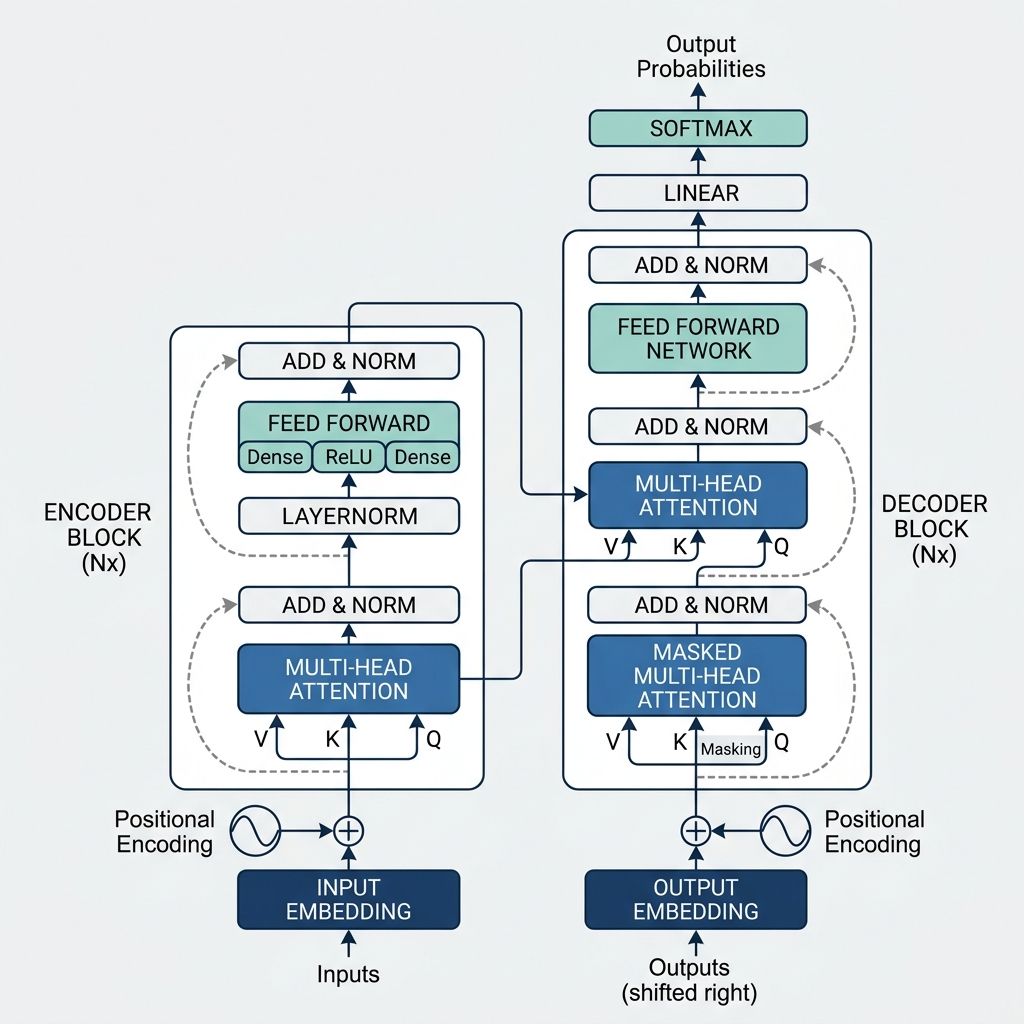
\includegraphics[width=0.8\textwidth]{Figures/transformer_architecture}
\caption{Transformer model architecture}
\label{fig:transformer_architecture}
\end{figure}

\subsection{BERT Pre-Training and Fine-Tuning}
BERT (Bidirectional Encoder Representations from Transformers) \cite{ref8} is a transformer encoder pre-trained on two self-supervised tasks: Masked Language Modelling (MLM) and Next Sentence Prediction (NSP). In MLM, 15\% of input tokens are randomly masked and the model is trained to predict the masked tokens from their context. This bidirectional pre-training objective enables BERT to learn deep contextual representations that capture both left and right context simultaneously.

Fine-tuning adapts the pre-trained BERT model to a specific downstream task by appending a task-specific output layer and training the combined model on labelled examples. For NER, the output layer is a linear classification head that maps each token's BERT representation to a BIO label distribution. Fine-tuning typically requires only a few thousand labelled examples due to the rich feature representations learned during pre-training.

\subsection{BioBERT for Biomedical NLP}
BioBERT \cite{ref1} initializes from the BERT-base weights and continues pre-training on approximately 4.5 billion words from PubMed abstracts and 13.5 billion words from PMC full-text articles. This domain-adaptive pre-training exposes the model to biomedical terminology, clinical abbreviations, and domain-specific syntactic patterns, resulting in significantly improved performance on biomedical NER, relation extraction, and question answering tasks compared to BERT trained exclusively on general-domain text.

For clinical NER tasks using the i2b2 datasets, BioBERT achieves $F_1$-scores of 0.886 on the 2010 dataset and 0.895 on the 2012 dataset, outperforming previous state-of-the-art systems by 2--4 percentage points.

\section{SNOMED CT: Structure and Coding Principles}
SNOMED CT (Systematized Nomenclature of Medicine --- Clinical Terms) is one of the most comprehensive and widely adopted clinical terminology systems used for representing medical concepts in a standardized manner. It provides a structured framework for organizing clinical knowledge and enables semantic interoperability across healthcare systems. By using standardized codes and concept relationships, SNOMED CT facilitates consistent representation of diagnoses, procedures, findings, medications, and other clinical entities. In the proposed Intelligent Clinical Document Processing System (ICDPS), SNOMED CT plays a critical role in transforming extracted clinical information into standardized representations that can support efficient storage, retrieval, and interoperability. The following sections discuss the ontology structure of SNOMED CT and the principles involved in the coding process. 

\subsection{Ontology Structure}
SNOMED CT is a formally structured clinical terminology comprising three primary components: Concepts, Descriptions, and Relationships. A Concept is a unique clinical idea identified by a numeric concept identifier (\texttt{conceptId}). Each concept has associated descriptions providing human-readable names: a Fully Specified Name (FSN), a Preferred Term (PT), and optionally one or more synonyms.

Relationships between concepts encode semantic associations. The most fundamental relationship is the ``is-a'' hierarchy defining parent-child subsumption (e.g., ``Type 2 diabetes mellitus'' is-a ``Diabetes mellitus''). Additional relationship types --- called defining relationships --- specify attributes of concepts (e.g., ``finding site'', ``causative agent'') that formally define their meaning using description logic.

SNOMED CT is organized into hierarchies including Clinical Finding, Procedure, Observable Entity, Body Structure, Organism, Substance, Pharmaceutical/Biologic Product, and Qualifier Value. These hierarchies correspond to the entity categories recognized by the ICDPS extraction engine.

\subsection{SNOMED CT Coding Process}
Clinical coding with SNOMED CT requires selecting the most specific concept that accurately represents the clinical entity described in the source document. This process involves:
\begin{enumerate}
    \item[(i)] identifying the target entity type (finding, procedure, substance, etc.);
    \item[(ii)] retrieving candidate concepts from the SNOMED CT release; and
    \item[(iii)] selecting the concept whose FSN and synonyms best match the clinical context.
\end{enumerate}

Automated SNOMED CT coding systems must contend with several challenges: synonym variability (multiple clinical terms may map to the same concept), compositional expressions (clinical descriptions may combine multiple SNOMED CT concepts), and contextual sensitivity (the appropriate code may depend on information outside the entity mention itself, such as negation status, laterality, or severity).

\section{Document Understanding and OCR}
Clinical documents are often available in diverse formats such as scanned reports, PDFs, image-based records, and structured templates, requiring efficient methods for extracting machine-readable information. Document understanding combines computer vision and natural language processing techniques to identify document structure, reading order, and semantic content. Optical Character Recognition (OCR) forms an essential component of this process by converting textual information embedded in images into digital text suitable for downstream processing. Additionally, semantic retrieval mechanisms such as vector similarity search improve the identification and mapping of extracted concepts. The following subsections discuss OCR techniques and vector-based retrieval methods used in the proposed system.

\subsection{Optical Character Recognition}
Optical Character Recognition (OCR) converts images of printed or handwritten text into machine-readable character sequences. Modern OCR engines such as Tesseract 5.0 \cite{ref36} use LSTM-based sequence models trained on large character recognition datasets. The OCR pipeline comprises image preprocessing (binarization, deskewing, noise removal), layout analysis (identifying text regions, columns, and reading order), and character recognition (generating character sequences from text regions).

OCR performance on clinical documents varies significantly with document quality. Printed clinical letters typically achieve character error rates below 2\%, while aged or low-quality scans may exhibit higher error rates. Post-OCR error correction using clinical dictionaries improves text quality for downstream NLP tasks.

\subsection{Vector Similarity Search}
Vector similarity search is used in the SNOMED CT candidate retrieval module to find concepts whose text descriptions are semantically similar to the extracted clinical entity. Each SNOMED CT concept description is represented as a dense vector using FastText embeddings \cite{ref17}, and an approximate nearest-neighbour search using FAISS (Facebook AI Similarity Search) retrieves the top-$K$ most similar candidates based on cosine similarity.

FAISS provides efficient indexing and retrieval for high-dimensional vector collections using quantization and graph-based algorithms. For the SNOMED CT index containing approximately 1.5 million concept descriptions, FAISS enables sub-second retrieval with approximate search accuracy exceeding 98\% relative to exact search.

\section{Mathematical Foundations}
The implementation of transformer-based language models and clinical entity extraction systems relies on several mathematical concepts that govern model learning and performance evaluation. Mathematical formulations provide the basis for converting model outputs into probability distributions, optimizing learning processes, and assessing predictive performance. Concepts such as loss functions, optimization strategies, and evaluation metrics are essential for understanding how the proposed system learns meaningful representations from clinical text and measures its effectiveness. The following subsections discuss the mathematical principles employed in the proposed framework. 

\subsection{Softmax and Cross-Entropy Loss}
The NER classification head applies the softmax function to convert raw logit scores into a probability distribution over BIO labels:
\begin{equation}
P(y = k \mid x) = \frac{\exp(z_k)}{\sum_{j} \exp(z_j)}
\label{eq:softmax}
\end{equation}
where $z_k$ is the logit for class $k$. The model is trained to minimize the cross-entropy loss:
\begin{equation}
\mathcal{L} = -\sum_{i=1}^{N} \log P(y = y_i \mid x_i)
\label{eq:cross_entropy}
\end{equation}
where $y_i$ is the true label for token $i$. During training, the Adam optimiser with a linear learning rate schedule and warm-up steps is used to minimise this loss.

\subsection{Evaluation Metrics}
NER performance is evaluated using token-level precision ($P$), recall ($R$), and F1-score ($F1$):
\begin{equation}
P = \frac{\text{TP}}{\text{TP} + \text{FP}}
\label{eq:precision}
\end{equation}
\begin{equation}
R = \frac{\text{TP}}{\text{TP} + \text{FN}}
\label{eq:recall}
\end{equation}
\begin{equation}
F1 = \frac{2 \cdot P \cdot R}{P + R}
\label{eq:f1_score}
\end{equation}
where TP is the number of correctly predicted entity tokens, FP the number of incorrectly predicted entity tokens, and FN the number of entity tokens missed by the model. SNOMED CT mapping performance is evaluated using $\text{Precision}@K$, which measures the proportion of test instances where the correct SNOMED CT code appears in the top-$K$ suggestions.

\section{Comparison of Techniques}
Various approaches have been proposed for clinical information extraction and natural language processing tasks, ranging from traditional rule-based systems to modern transformer-based architectures. Each technique exhibits distinct characteristics in terms of training requirements, generalization capability, computational complexity, and overall performance. A comparative analysis of these techniques helps in understanding their strengths and limitations and provides a rationale for selecting an appropriate methodology for the proposed system. Table \ref{tab:ner_techniques_comparison} presents a comparison of commonly used approaches, including rule-based systems (e.g., cTAKES \cite{ref6}), BiLSTM-CRF models, and transformer-based methods across multiple evaluation criteria.

\begin{table}[htbp]
\centering
\caption{Comparison of Clinical NER Techniques}
\label{tab:ner_techniques_comparison}

\begin{tabular}{|p{3cm}|p{3.65cm}|p{3.75cm}|p{3.8cm}|}
\hline

\textbf{Criterion} &
\shortstack{\textbf{Rule-Based}\\\textbf{(cTAKES)}} &
\textbf{BiLSTM-CRF} &
\shortstack{\textbf{Transformer}\\\textbf{(BioBERT)}} \\

\hline

Training Data Required &
None (rules only) &
Moderate (annotated) &
Large (pre-training) + small (fine-tuning) \\

\hline

Generalization &
Low (template-dependent) &
Moderate &
High \\

\hline

Domain Adaptation &
Manual rule updates &
Re-training required &
Fine-tuning on small dataset \\

\hline

Clinical NER $F1$ &
0.72--0.78 &
0.80--0.85 &
0.88--0.93 \\

\hline

OOV Handling &
Poor &
Moderate (char features) &
Good (subword tokenization) \\

\hline

Inference Speed &
Fast &
Moderate &
Slower (GPU recommended) \\

\hline
\end{tabular}

\end{table}

\section*{Summary}
This chapter presented the theoretical foundations of the ICDPS, covering NLP fundamentals, the transformer architecture, BERT-based biomedical pre-training, SNOMED CT ontology structure, OCR technology, vector similarity search, and the mathematical principles underlying model training and evaluation. The comparative analysis demonstrated the superiority of transformer-based approaches over rule-based and BiLSTM-CRF methods for clinical NER tasks. Chapter 3 presents the detailed software requirements specification for the proposed system.

		
		%Chapter 3
		\chapter{Software Requirement Specification}

The Software Requirement Specification (SRS) defines the operational requirements and constraints of the Intelligent Clinical Document Processing System (ICDPS). Establishing these requirements is necessary to ensure that the implemented system aligns with the objectives of clinical document processing, information extraction, summarization, and SNOMED CT terminology mapping described in previous chapters.

The proposed system integrates multiple processing components within a unified workflow, including document ingestion, OCR, clinical entity extraction, semantic retrieval, and structured output generation. Each component introduces specific requirements related to functionality, performance, reliability, security, and usability. These requirements serve as a reference for subsequent design, implementation, and evaluation activities.

This chapter describes the functional and non-functional requirements of the system together with the hardware, software, and operational conditions considered during development and deployment.

\section{Overall Description}

The Intelligent Clinical Document Processing System (ICDPS) is designed to transform unstructured clinical documents into structured information suitable for review and terminology coding. Users submit clinical documents to the system, which then processes the content through a sequence of extraction, analysis, and coding stages before presenting the resulting information through a review interface.

The system supports the processing of both digitally generated and image-based clinical documents. Its primary outputs include extracted clinical entities, generated summaries, and confidence-ranked SNOMED CT coding suggestions. The architecture is intended to operate as an intermediary processing layer between document sources and downstream healthcare applications.

This section outlines the operating environment, principal system functions, user interactions, and design constraints that define the scope and expected behaviour of the proposed solution.

\subsection{Product Perspective}

The Intelligent Clinical Document Processing System (ICDPS) was designed as a standalone server-side application responsible for processing clinical documents and generating structured outputs. Rather than being developed for a specific Electronic Health Record (EHR) platform, the system operates independently and can be integrated with existing healthcare applications through REST-based interfaces.

Clinical documents are submitted to the processing pipeline, where they undergo document ingestion, text extraction, information extraction, summarization, and SNOMED CT mapping. The resulting entities, summaries, and coding suggestions are then returned to the requesting application through the API. By separating document processing from external healthcare systems, the architecture supports integration with different document repositories, review interfaces, and coding workflows without requiring modifications to the core pipeline.

The system was designed for deployment within a secure healthcare environment. Communication between components is protected using TLS 1.3 encryption, while processed documents and generated outputs are stored in a PostgreSQL database to support auditing, validation, and review activities. All processing is performed within the deployment environment, ensuring that patient information remains within organizational boundaries throughout the workflow.

\subsection{Product Functions}
The ICDPS provides the following functionalities:
\begin{itemize}
    \item \textbf{Document Ingestion:} Accept clinical documents in PDF and image formats through API-based uploads or batch document processing workflows.
    \item \textbf{Text Extraction:} Extract machine-readable text from PDFs using direct extraction; apply OCR to image-based documents.
    \item \textbf{Named Entity Recognition:} Identify and classify clinical entities in extracted text across eight predefined categories.
    \item \textbf{Clinical Summarization:} Generate extractive summaries of clinical documents highlighting key findings.
    \item \textbf{Role-Based Categorization:} Assign extracted entities to clinical role action categories (Pharmacist, Clinician, Radiologist, etc.).
    \item \textbf{SNOMED CT Suggestion:} Retrieve and rank candidate SNOMED CT codes for each extracted entity, presenting the top-5 suggestions with confidence scores.
    \item \textbf{Interactive Review Interface:} Provide a web-based interface for authorized clinicians and coders to review, accept, modify, or reject suggested codes.
    \item \textbf{Audit Logging:} Record all processing events and user actions for compliance and quality assurance purposes.
\end{itemize}

\subsection{User Characteristics}
The ICDPS is intended for two primary user categories:
\begin{itemize}
    \item \textbf{Clinical Coders:} Staff responsible for assigning SNOMED CT codes to clinical documents. Typically possess clinical coding training but may have limited technical expertise. Interact with the system via the web-based review interface.
    \item \textbf{System Administrators:} Technical staff responsible for system configuration, monitoring, and maintenance. Possess technical expertise and access system management functions via command-line and configuration interfaces.
\end{itemize}

\subsection{Constraints}
The following constraints apply to the ICDPS:
\begin{itemize}
    \item \textbf{Data Privacy:} All processing must comply with the UK General Data Protection Regulation (UK GDPR) and NHS Data Security and Protection Toolkit requirements. Personally identifiable patient data must not be transmitted outside the clinical network.
    \item \textbf{Hardware Dependency:} Optimal NER performance requires a CUDA-compatible GPU with at least 8 GB VRAM. CPU-only operation is supported but with reduced inference speed.
    \item \textbf{SNOMED CT Licensing:} SNOMED CT is licensed by SNOMED International. Use of SNOMED CT requires a valid SNOMED CT licence. The system incorporates the UK Edition of SNOMED CT, requiring an NHS licence.
    \item \textbf{Language Limitation:} The current version supports English-language documents only. Multilingual support is identified as a future enhancement.
    \item \textbf{OCR Accuracy:} OCR performance is dependent on document scan quality. Documents with resolution below 150 DPI may exhibit degraded extraction quality.
\end{itemize}

\section{Specific Requirements}

This section outlines the requirements identified for the Intelligent Clinical Document Processing System (ICDPS). These requirements describe the expected functionality of the system, its operational characteristics, and the constraints considered during development. They establish the criteria against which the system is designed, implemented, and evaluated.

\subsection{Functional Requirements}

The functional requirements define the primary capabilities expected from the ICDPS. They describe how the system processes clinical documents, extracts and organizes information, generates SNOMED CT coding suggestions, and presents results for user review. Table~\ref{tab:functional_requirements} summarizes these requirements and their implementation priority.

\begin{longtable}{|p{1.4cm}|p{10.4cm}|p{2cm}|}
\caption{Functional Requirements}
\label{tab:functional_requirements} \\
\hline
\textbf{FR ID} & \textbf{Requirement Description} & \textbf{Priority} \\
\hline
\endfirsthead
\hline
\textbf{FR ID} & \textbf{Requirement Description} & \textbf{Priority} \\
\hline
\endhead
\hline
\endfoot
FR-01 & The system shall accept clinical documents in PDF, JPEG, PNG, and TIFF formats via REST API upload. & High \\
\hline
FR-02 & The system shall extract machine-readable text from PDFs using direct text extraction without OCR. & High \\
\hline
FR-03 & The system shall apply OCR to image-format documents using the Tesseract 5.0 engine to generate UTF-8 text. & High \\
\hline
FR-04 & The system shall automatically detect and classify clinical entities from processed document text into predefined categories such as Diagnosis, Medication, Dosage, Procedure, Anatomy, Allergy, Laboratory Result, and Temporal Expression. & High \\
\hline
FR-05 & The system shall assign a negation status (affirmed/negated/uncertain) to each identified entity. & High \\
\hline
FR-06 & The system shall generate an extractive clinical summary comprising the most clinically significant sentences from the document. & Medium \\
\hline
FR-07 & The system shall assign each extracted entity to a role-specific action category (Pharmacist Action, Clinician Review, Radiologist Review, or General Information). & High \\
\hline
FR-08 & The system shall retrieve the top-5 SNOMED CT concept candidates for each affirmed entity using vector similarity search, ranked by confidence score. & High \\
\hline
FR-09 & The system shall present SNOMED CT suggestions with the concept identifier, preferred term, and confidence score through the review interface. & High \\
\hline
FR-10 & The system shall allow authorized users to accept, modify, or reject SNOMED CT suggestions through the web interface. & High \\
\hline
FR-11 & The system shall log all processing events and user code selection actions with timestamps for audit purposes. & Medium \\
\hline
FR-12 & The system shall support batch processing of multiple documents submitted as a directory archive. & Medium \\
\hline
FR-13 & The system shall return processing results in JSON format through the REST API. & High \\
\hline
FR-14 & The system shall provide an exportable structured report in CSV format summarizing extracted entities and accepted SNOMED CT codes. & Medium \\
\hline
\end{longtable}

\subsection{Non-Functional Requirements}

Non-functional requirements specify the performance and operational characteristics expected from the ICDPS. They address factors such as reliability, security, usability, maintainability, and processing efficiency, which influence the overall quality and dependability of the system. The non-functional requirements considered during system development are presented in Table~\ref{tab:nonfunctional_requirements}.

\begin{longtable}{|p{1.8cm}|p{2.6cm}|p{10cm}|}
\caption{Non-Functional Requirements}
\label{tab:nonfunctional_requirements} \\
\hline
\textbf{NFR ID} & \textbf{Category} & \textbf{Requirement Description} \\
\hline
\endfirsthead
\hline
\textbf{NFR ID} & \textbf{Category} & \textbf{Requirement Description} \\
\hline
\endhead
\hline
\endfoot
NFR-01 & Performance & The system shall complete NER processing of a single-page clinical document within 3 seconds on hardware meeting the minimum specification. \\
\hline
NFR-02 & Throughput & The system shall support batch processing of at least 100 documents per hour during standard operation. \\
\hline
NFR-03 & Accuracy & The NER module shall achieve a token-level F1-score of at least 0.85 on the system test corpus across all eight entity categories. \\
\hline
NFR-04 & SNOMED Precision & The SNOMED CT mapping module shall achieve a precision@1 value of at least 0.85 on the SNOMED test dataset. \\
\hline
NFR-05 & Security & All API communications shall use TLS 1.3 encryption. User authentication shall use JWT tokens with a 24-hour expiry period. \\
\hline
NFR-06 & Availability & The system shall maintain 99\% uptime during scheduled operational hours (08:00--20:00 weekdays). \\
\hline
NFR-07 & Usability & The review interface shall be usable by clinical coders with minimal technical training. \\
\hline
NFR-08 & Maintainability & The system shall support modular architecture and documented APIs for easier updates and maintenance. \\
\hline
NFR-09 & Portability & The system shall be containerized using Docker and deployable on compatible Linux environments. \\
\hline
\end{longtable}

\subsection{Performance Requirements}

Performance requirements define the expected processing speed and responsiveness of the Intelligent Clinical Document Processing System (ICDPS). These requirements establish operational targets for the major processing components and help ensure that clinical documents can be analysed within acceptable time limits.

The NER module is expected to process approximately 500 tokens per second on a system equipped with an NVIDIA A100 GPU. The SNOMED CT candidate retrieval module should return the top five concept suggestions within 200 milliseconds for each entity query. In addition, the web-based review interface should display extraction results for an individual clinical document within 2 seconds on a standard clinical workstation.

The system should maintain stable performance when processing larger documents containing up to 50 pages or approximately 25,000 tokens. These performance targets were selected to support efficient document processing while maintaining a responsive user experience during review and coding activities.

\subsection{Software Requirements}

Software requirements define the software components and technologies used within the ICDPS framework. The selected libraries, frameworks, and development tools support the implementation of document processing workflows, machine learning inference, database operations, and system deployment activities.

Table~\ref{tab:software_requirements} summarizes the software platforms, development environments, and supporting technologies used in the implementation of the Intelligent Clinical Document Processing System (ICDPS).

\begin{longtable}{|p{4.5cm}|p{9cm}|}
\caption{Software Requirements}
\label{tab:software_requirements}\\

\hline
\textbf{Category} &
\textbf{Specification} \\
\hline
\endfirsthead

\hline
\textbf{Category} &
\textbf{Specification} \\
\hline
\endhead

\hline
\multicolumn{2}{r}{Continued on next page} \\
\endfoot

\hline
\endlastfoot


Operating System &
Ubuntu 22.04 LTS (Server), Windows 10+ (Client browser) \\
\hline

Programming Language &
Python 3.10 \\
\hline

NLP Framework &
Hugging Face Transformers 4.38, PyTorch 2.0 \\
\hline

OCR Engine &
Tesseract 5.0 with LSTM models \\
\hline

PDF Processing &
PyMuPDF 1.23 \\
\hline

Vector Search &
FAISS 1.7 \\
\hline

Web Framework &
Flask 3.0 \\
\hline

Database &
PostgreSQL 16 \\
\hline

Containerization &
Docker 24, Docker Compose 2 \\
\hline

Development IDE &
PyCharm / Visual Studio Code \\
\hline

Version Control &
Git / GitHub \\
\hline

\end{longtable}

\subsection{Hardware Requirements}
The performance and efficiency of the proposed system are significantly influenced by the underlying hardware infrastructure used during development and deployment. Hardware requirements define the minimum and recommended computational resources needed for processing clinical documents, executing transformer-based models, and supporting large-scale data operations. Table~\ref{tab:hardware_requirements} presents the hardware specifications required for effective implementation and system execution.

\begin{longtable}{|p{3.6cm}|p{5.5cm}|p{4.2cm}|}
\caption{Hardware Requirements}
\label{tab:hardware_requirements}\\

\hline
\textbf{Component} &
\textbf{Minimum Specification} &
\textbf{Recommended Specification} \\
\hline
\endfirsthead

\hline
\textbf{Component} &
\textbf{Minimum Specification} &
\textbf{Recommended Specification} \\
\hline
\endhead

\hline
\multicolumn{3}{r}{Continued on next page} \\
\endfoot

\hline
\endlastfoot


Processor &
Intel Core i7 (8 cores) &
Intel Xeon (16+ cores) \\
\hline

RAM &
16 GB DDR4 &
64 GB DDR4 \\
\hline

GPU &
NVIDIA GTX 1080 (8 GB VRAM) &
NVIDIA A100 (40 GB VRAM) \\
\hline

Storage &
500 GB SSD &
2 TB NVMe SSD \\
\hline

Network &
1 Gbps Ethernet &
10 Gbps Ethernet \\
\hline

Operating System &
Ubuntu 22.04 LTS &
Ubuntu 22.04 LTS \\
\hline

\end{longtable}

\subsection{Design Constraints}
Design constraints define the technical and operational limitations that influence the architecture, implementation, and deployment of the proposed Intelligent Clinical Document Processing System (ICDPS). The following are the design constraints of ICDPS:
\begin{itemize}
    \item \textbf{Platform Dependency:} The NER module requires CUDA-compatible GPU hardware for production-grade throughput. CPU-only deployment is limited to low-volume testing scenarios.
    \item \textbf{Memory Constraints:} Loading the BioBERT model requires approximately 1.5 GB of GPU VRAM. Simultaneous processing of multiple documents requires proportional VRAM scaling.
    \item \textbf{SNOMED CT Index Size:} The FAISS index for SNOMED CT concept descriptions occupies approximately 3.5 GB of disk space and 6 GB of RAM when loaded.
    \item \textbf{Network Security:} The system must operate within a network that enforces NHS Data Security and Protection Toolkit controls, restricting external API calls.
    \item \textbf{SNOMED CT Licence Compliance:} The system must not distribute SNOMED CT content beyond the licensed deployment site.
\end{itemize}

\section*{Summary}

This chapter outlined the software requirements of the ICDPS, covering functional requirements, non-functional requirements, performance targets, operational constraints, and the supporting technologies required for deployment. These requirements define the expected behaviour and operating environment of the proposed system.

The next chapter focuses on the high-level system architecture and explains how the identified requirements influenced the design of the overall processing framework.

		
		%Chapter 4
		\chapter{High-Level Design}

The Intelligent Clinical Document Processing System (ICDPS) consists of multiple components that work together to process clinical documents, extract relevant information, generate summaries, and map identified entities to SNOMED CT concepts. To support these operations, the system is organized as a modular processing pipeline in which each component performs a specific task and passes its output to the next stage.

This chapter describes the overall architecture of the proposed system, the design principles considered during development, and the high-level interactions between major modules. The architecture provides a framework for understanding how clinical documents move through the system from ingestion to final review and coding.

\section{Design Considerations}

Several design considerations influenced the architecture of the ICDPS. Since clinical documents may vary in format, content, and quality, the system was designed to support flexible document processing while maintaining reliability and ease of maintenance. Additional considerations included scalability, security, modularity, and support for future extensions.

These factors guided the selection of technologies, deployment strategies, and interactions between individual system components.

\subsection{General Considerations}

The architectural design of the ICDPS was guided by the following engineering principles:

\begin{itemize}

\item \textbf{Modularity:} The system is decomposed into independently deployable modules --- Document Ingestion, Text Extraction, NER Engine, Summarization Engine, SNOMED CT Mapper, and Review Interface --- each with well-defined input and output contracts. This modular structure supports component-level testing, independent updates, and replacement of individual technologies without affecting the entire system.

\item \textbf{Scalability:} The processing pipeline supports horizontal scaling through containerized deployment. Additional processing instances can be introduced when document throughput requirements increase.

\item \textbf{Reliability:} Error-handling mechanisms are incorporated at each stage of the pipeline. Documents that fail processing are redirected to an error queue for review, and processing events are recorded for auditing and troubleshooting.

\item \textbf{Maintainability:} Modules are documented using API specifications and maintained within a version-controlled repository. Configuration files and model weights are managed separately from application code to simplify updates and maintenance.

\item \textbf{Security:} Role-based access control is enforced for system interfaces and API endpoints. Clinical documents and extracted information are processed within the deployment environment, with access restricted to authorized users.

\item \textbf{Explainability:} SNOMED CT code suggestions are accompanied by confidence scores, and extracted entities are linked to their corresponding text spans to support user review and verification.

\end{itemize}

\subsection{Development Methodology}

Development followed an iterative Software Development Life Cycle (SDLC) consisting of requirements analysis, system design, implementation, testing, and deployment preparation. This approach allowed individual components to be developed and evaluated incrementally, with modifications introduced based on intermediate testing and performance results.

Agile development practices, including periodic sprint reviews, version control, and continuous integration through GitHub Actions, were used to monitor progress and manage development activities throughout the project.

\section{Architecture Strategies}

Architecture strategies describe the structural and technological approaches used in the development of the proposed system. These decisions influence how components communicate, how data moves through the processing pipeline, and how the system can be extended or deployed in different environments.

The selected architecture combines document processing, NLP, semantic retrieval, and terminology mapping within a modular framework. This design allows individual components to be updated independently while maintaining compatibility with the overall processing workflow.

\subsection{Technology and Framework Selection}
Python 3.10 was chosen as the primary implementation language because of its extensive support for machine learning, natural language processing, and data processing libraries. It also provides compatibility with the frameworks and tools used throughout the project. The Hugging Face Transformers library was selected as the primary NLP framework because it offers well-documented implementations of BioBERT and other transformer-based models, along with standardized interfaces for training and inference.

PyMuPDF was selected for PDF text extraction due to its superior text extraction fidelity on complex clinical PDF layouts compared to alternatives such as pdfplumber and PDFMiner. Tesseract 5.0 was selected for OCR because it supports LSTM-based recognition with NHS-relevant font coverage and is available under a free and open-source licence.

FAISS was selected for SNOMED CT vector search because it provides both exact and approximate nearest-neighbour search with GPU acceleration support, enabling sub-second retrieval from the 1.5 million concept description index. Flask was selected for the web interface due to its lightweight architecture suitable for the single-institution deployment context.

\subsection{Scalability and Future Enhancements}
The containerized architecture supports future deployment on cloud infrastructure (NHS-approved cloud providers). Additional NLP models supporting ICD-10 or LOINC coding could be integrated as independent modules without modifying the core pipeline. The SNOMED CT index can be updated to reflect new SNOMED CT releases by rerunning the index construction script with the new release files.

Future enhancements identified include:
\begin{enumerate}[(i)]
    \item real-time API integration with NHS EHR systems;
    \item support for handwritten clinical note processing using dedicated handwriting recognition models;
    \item multilingual support for Welsh and other NHS-relevant languages; and
    \item active learning integration to continuously improve extraction performance using clinician feedback.
\end{enumerate}

\section{Overall System Architecture}

The Intelligent Clinical Document Processing System (ICDPS) processes clinical documents through a sequence of interconnected stages that transform raw documents into structured clinical information and SNOMED CT coding suggestions. The system is designed to handle documents originating from different sources, including scanned reports, referral letters, discharge summaries, and other healthcare records that may vary in format and quality.

To support this workflow, the architecture is organized into multiple processing layers. Each layer performs a specific task and passes its output to the next stage of the pipeline. This modular structure simplifies development and testing while allowing individual components to be updated or replaced without affecting the overall workflow.

\subsection{High-Level Architecture Diagram}

Figure~\ref{fig:hla_diagram} illustrates the overall processing workflow of the ICDPS. The workflow begins with document ingestion and concludes with the presentation of extracted information, summaries, and coding suggestions through the NHS Portal interface. The architecture is organized into six primary processing layers, each responsible for a distinct stage of document analysis.

\textbf{Layer 1 --- Document Ingestion and Rendering} receives uploaded clinical documents through the NHS Portal interface. Documents are processed by the \texttt{document\_handler} module and routed to PyMuPDF for page-level rendering and conversion into PNG images for downstream processing.
\textbf{Layer 2 --- Image Preprocessing} uses OpenCV to improve image quality before OCR processing. Operations such as adaptive thresholding, noise reduction, and deskewing are applied to improve text visibility and document consistency.

\textbf{Layer 3 --- OCR Extraction and Confidence Routing} uses AWS Textract to extract document text and confidence values. Documents with confidence scores above the predefined threshold continue through the standard processing path, while lower-confidence outputs are forwarded to a LayoutLMv3 refinement stage.

\textbf{Layer 4 --- Entity Extraction and Clinical Coding} identifies clinically relevant entities and maps extracted concepts to SNOMED CT terminology using the clinical coding pipeline.

\textbf{Layer 5 --- PHI Detection, Structured Field Extraction, and Summarisation} detects protected health information (PHI), extracts structured fields, and generates summaries tailored to different user roles.

\textbf{Layer 6 --- Confidence Aggregation and Output Rendering} combines confidence measures from multiple processing stages to calculate a Unified Confidence Score (UCS) and presents the final results through the NHS Portal interface.

\begin{figure}[htbp]
\centering
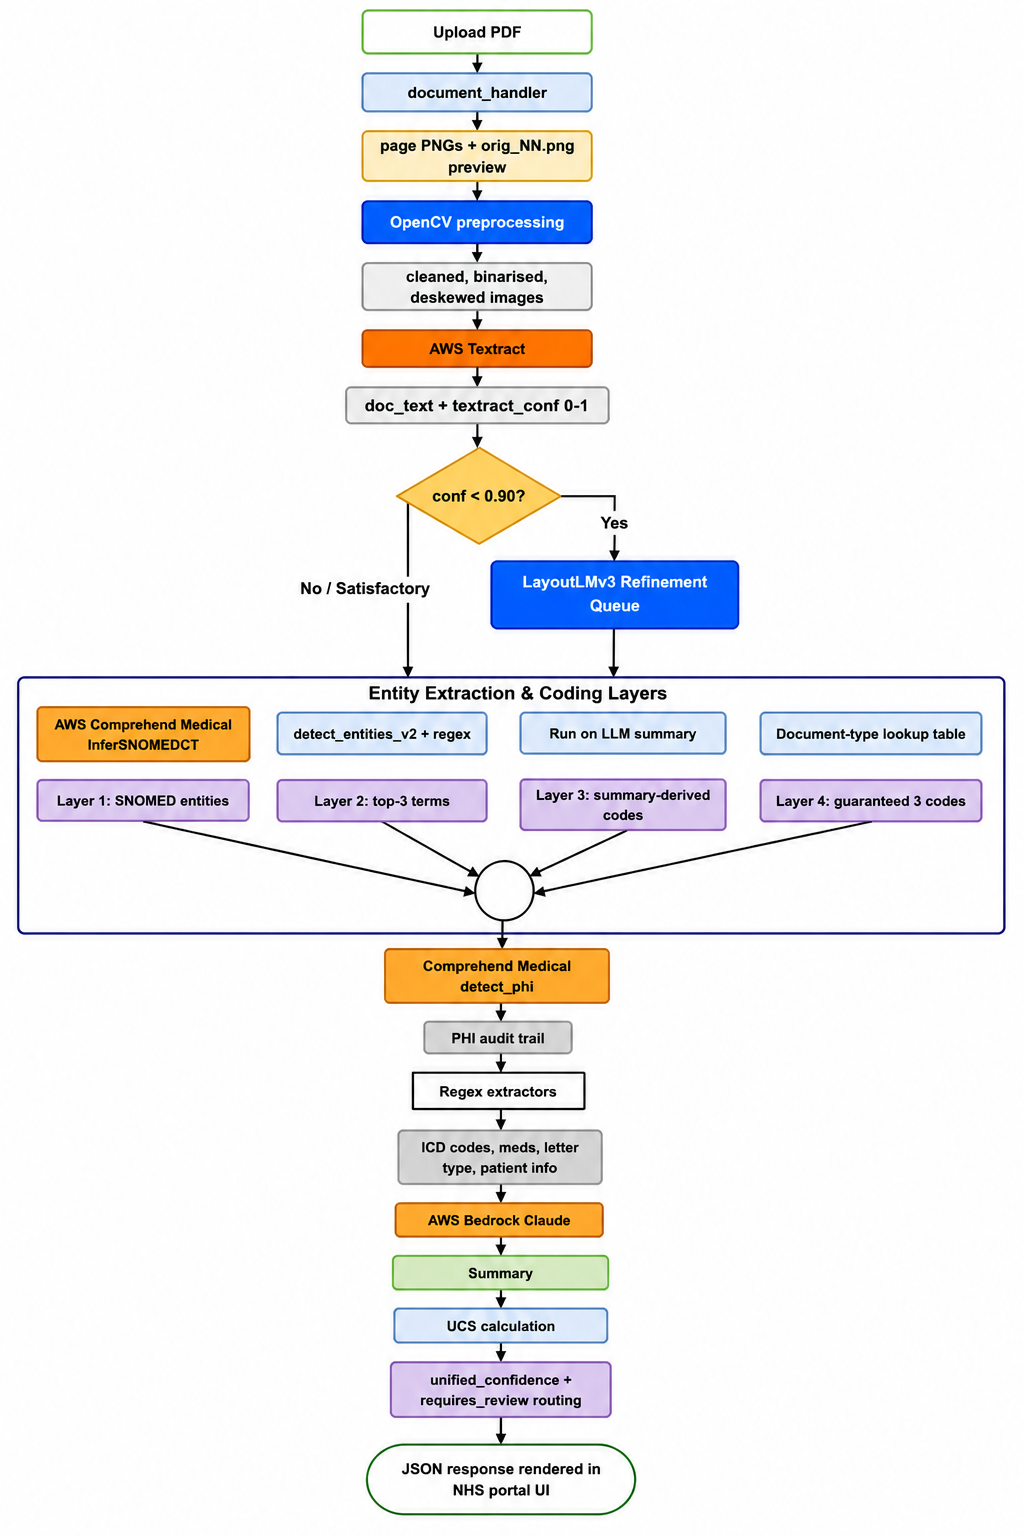
\includegraphics[width=\textwidth]{Figures/hla_diagram.png}
\caption{High-Level Architecture Diagram of the ICDPS six-layer processing pipeline.}
\label{fig:hla_diagram}
\end{figure}

\subsection{Module Description}

The ICDPS consists of a set of modules that collectively implement the document processing workflow. Each module is responsible for a specific stage of processing and exchanges information with other components through predefined interfaces. This separation allows individual modules to be modified, optimized, or extended independently as the system evolves.

Table~\ref{tab:module_descriptions} summarizes the major modules in the architecture, along with their inputs, processing responsibilities, and generated outputs.

\begin{longtable}{|>{\raggedright\arraybackslash}p{3.3cm}|
                  >{\raggedright\arraybackslash}p{2.7cm}|
                  >{\raggedright\arraybackslash}p{3.9cm}|
                  >{\raggedright\arraybackslash}p{3.9cm}|}
\caption{ICDPS Module Descriptions}
\label{tab:module_descriptions} \\
\hline
\textbf{Module} & \textbf{Input} & \textbf{Processing} & \textbf{Output} \\
\hline
\endfirsthead
\hline
\textbf{Module} & \textbf{Input} & \textbf{Processing} & \textbf{Output} \\
\hline
\endhead
\hline
\endfoot
\texttt{document\_handler} & PDF / JPEG / PNG / TIFF & PyMuPDF rendering; file type routing & PNG page images; \texttt{orig\_NN.png} previews \\
\hline
OpenCV Preprocessor & Raw page PNGs & Adaptive threshold; MORPH\_CLOSE; deskew & Cleaned, binarised, aligned PNGs \\
\hline
AWS Textract OCR & Preprocessed PNGs & AnalyzeDocument API; block parsing & \texttt{doc\_text}; \texttt{textract\_conf} (0--1) \\
\hline
Confidence Router & \texttt{textract\_conf} & Threshold comparison vs.\ 0.90 & Route to LayoutLMv3 or continue \\
\hline
LayoutLMv3 Refiner & Low-conf page images & Multi-modal transformer inference & Corrected text blocks \\
\hline
SNOMED Mapper (4-layer) & \texttt{doc\_text}; entities; summary & InferSNOMEDCT; regex; lookup table & SNOMED codes with confidence \\
\hline
PHI Detector & \texttt{doc\_text} & Comprehend Medical DetectPHI & \texttt{phi\_entities} list; audit trail \\
\hline
Regex Extractor & \texttt{doc\_text} & Pattern matching for ICD-10, meds & \texttt{icd\_codes}; medications; patient info \\
\hline
Bedrock Claude LLM & \texttt{doc\_text} + SNOMED entities & Role-specific prompts; prose generation & 3 role-specific summaries \\
\hline
UCS Calculator & \texttt{textract\_conf}; \texttt{snomed\_conf}; \texttt{llm\_conf} & Weighted formula by document type & \texttt{unified\_confidence}; review routing \\
\hline
NHS Portal UI & JSON result dict & JavaScript / React rendering & Interactive clinical review interface \\
\hline
\end{longtable}

\subsection{High-Level AI Workflow}

The AI workflow within the ICDPS processes extracted document content through multiple analysis paths rather than a single sequential pipeline. After OCR extraction, the document content is routed to two independent processing tracks together with a confidence evaluation mechanism.

\begin{itemize}

\item \textbf{Track A} performs clinical entity extraction and terminology mapping. Extracted medical concepts are processed through the SNOMED CT safety-net architecture to identify appropriate standardized healthcare codes.

\item \textbf{Track B} performs clinical language understanding and document summarization. AWS Bedrock Claude Sonnet is used to generate contextual summaries tailored to different healthcare users and review scenarios.

\item \textbf{Confidence Scoring Layer} combines confidence values generated during OCR extraction, SNOMED CT mapping, and language model processing. These values are aggregated into a Unified Confidence Score (UCS), which is used to determine whether the generated output can proceed automatically or requires additional human review.

\end{itemize}

The separation of entity extraction and language understanding into independent processing tracks allows the system to continue producing useful outputs even when one component performs less effectively on a particular document.

\section{Data and Learning Workflow}

The ICDPS workflow describes how information moves through the system during both training and inference. Clinical documents are progressively transformed from raw uploaded files into structured entities, summaries, and SNOMED CT coding suggestions through a sequence of processing stages.

The workflow includes document ingestion, OCR processing, information extraction, terminology mapping, confidence evaluation, and output generation. Each stage produces intermediate results that are passed to downstream components, allowing individual modules to be evaluated, updated, and maintained independently.

The following sections describe the flow of data through the system and the learning processes used to train and evaluate the machine learning components.

\subsection{End-to-End Workflow Diagram}
The end-to-end workflow provides a comprehensive representation of the sequence of operations performed by ICDPS from document submission to final output generation. The complete process is divided into five major stages:

\begin{enumerate}
    \item Document Upload and Ingestion
    \item Image Preprocessing
    \item OCR Extraction and Confidence Routing
    \item Parallel Processing for Entity Extraction, PHI Detection, and Summarisation
    \item Confidence Aggregation and Output Rendering
\end{enumerate}

Each stage produces outputs that are passed to downstream components, forming the overall document processing workflow. The process begins when a clinical document is uploaded through the NHS Portal interface. Document pages are rendered and enhanced before OCR extraction converts visual content into machine-readable text. Confidence-based routing is then used to determine whether additional processing through the LayoutLMv3 refinement module is required. After text extraction, multiple downstream tasks execute in parallel to reduce processing time and improve overall throughput.

\subsection{Training Workflow Overview}

Most components within the ICDPS rely on pre-trained models and managed services for OCR, language understanding, and terminology processing. As a result, large-scale model training is not required for every stage of the pipeline. However, the LayoutLMv3 refinement module was adapted for clinical document processing through task-specific fine-tuning.

The training workflow begins with the collection and preparation of NHS-style clinical documents. Documents are converted into annotated page images and associated with bounding-box information representing relevant text regions. The dataset is divided into training, validation, and testing subsets using a 70:15:15 split.

A pre-trained LayoutLMv3-base model is then fine-tuned using the AdamW optimizer together with cosine annealing learning-rate scheduling. Validation performance is evaluated throughout training, and early stopping is used to reduce overfitting. The checkpoint achieving the best validation performance is selected for deployment within the refinement stage of the production pipeline.

\subsection{Inference Workflow Overview}

The inference workflow describes how the deployed system processes newly submitted clinical documents. Unlike the training workflow, no model parameters are updated during this stage.

When a document is uploaded, it undergoes rendering and image preprocessing before being submitted to AWS Textract for OCR extraction. Documents with OCR confidence scores above the predefined threshold of 0.90 continue through the standard processing path. Documents falling below this threshold are routed to the LayoutLMv3 refinement module for additional processing.

Following text extraction, the SNOMED CT mapping cascade identifies medical concepts and generates standardized terminology suggestions. PHI detection, structured field extraction, and document summarization execute in parallel to improve processing efficiency. The resulting outputs are then combined with confidence measures from multiple stages to calculate the Unified Confidence Score (UCS). Based on this score, the system determines whether the generated results can proceed directly to output generation or should be flagged for clinician review.

\section{System Interaction and Deployment Overview}

This section describes how users interact with the ICDPS platform and how the system components operate within the deployment environment. In addition to document processing functionality, the platform must support secure data handling, responsive user interaction, and reliable execution of the processing pipeline. The deployment architecture combines containerized services and cloud infrastructure to support document processing, model inference, and workflow management.

\subsection{User Interaction Flow}

The NHS Portal UI serves as the primary interface through which healthcare users interact with the system. The interface supports document submission, review of generated outputs, and export of processed results.

When a document is uploaded, a multipart POST request initiates the backend processing workflow. Processing status is communicated through a progress indicator while the document moves through the pipeline. After processing is complete, results are presented through four tabbed views: Details, Coding, Follow-up, and GP Actions.

A colour-coded Unified Confidence Score badge provides a visual indication of output confidence. Users can review generated summaries, inspect extracted entities, modify SNOMED CT coding suggestions where necessary, and export the resulting structured records.

\subsection{Model-Service Interaction}

Communication between processing components is handled through secure service interfaces. The ICDPS backend interacts with AWS services through \texttt{boto3} clients using encrypted TLS connections and region-specific endpoints. Deploying related services within the same AWS region helps reduce communication latency and simplifies operational management.

Protected Health Information (PHI) is excluded from logging operations before audit records are stored. The LayoutLMv3 refinement component is deployed as a locally hosted containerized service, enabling independent inference and asynchronous processing of low-confidence documents.

\subsection{Deployment Overview}

The ICDPS deployment architecture uses a cloud-native approach built around containerized services and managed AWS infrastructure. The Flask backend and LayoutLMv3 inference service are packaged using Docker containers and deployed through Amazon ECS with Fargate support.

The NHS Portal frontend is distributed through CloudFront to improve availability and response times. Amazon SQS provides asynchronous communication between processing stages, while AWS Step Functions coordinate workflow execution and error-handling procedures. Audit records, extracted information, and processing metadata are stored in Amazon DynamoDB.

This deployment model separates processing responsibilities across multiple services while supporting scalability, fault tolerance, and operational flexibility.

\section*{Summary}

This chapter described the high-level architecture of the Intelligent Clinical Document Processing System (ICDPS), including the major processing layers, module interactions, AI workflow, deployment environment, and user interaction mechanisms. The design principles adopted during development and the technologies used to implement the architecture were also discussed.

The architecture provides a framework for understanding how clinical documents move through the system from ingestion to final output generation. The next chapter presents the detailed design of individual modules, including data organization, preprocessing workflows, model configurations, and implementation-level design decisions.

		
		%Chapter 5
		\chapter{Detailed Design}

This chapter presents the detailed design of the Intelligent Clinical Document Processing System (ICDPS). Building upon the high-level architecture described in the previous chapter, it examines the internal structure of individual components, the data flow between processing stages, and the design decisions that support system implementation.

The chapter covers dataset organisation, document preprocessing, model architecture, terminology mapping, training procedures, and inference workflows. Collectively, these elements define the technical processes through which clinical documents are transformed into structured information and SNOMED CT coding recommendations.

\section{Dataset and Data Organisation}

The implementation of the ICDPS required data resources supporting document understanding, clinical information extraction, and terminology mapping tasks. Effective organisation of these resources was necessary to support preprocessing, model development, evaluation, and validation activities throughout the project.

The datasets used in this work comprise clinical documents, annotation files, and supporting terminology resources. These datasets were organised to facilitate model training, testing, and performance assessment while maintaining a clear separation between development and evaluation data. This section describes the composition of the datasets, their organisational structure, and the data preparation procedures adopted during system development.

\subsection{Dataset Description}
The primary dataset comprises 40 real-world clinical documents obtained from Easthampstead Surgery, London, United Kingdom. These documents represent the full spectrum encountered in a typical NHS primary care workflow: outpatient correspondence, specialist referral letters, hospital discharge summaries, NHS 111 reports, Accident and Emergency summaries, ambulance service reports, diabetic eye screening reports, and out-of-hours primary care reports. The dataset includes both digitally generated PDF documents and scanned document images produced from photographed or photocopied clinical letters.

Each document contains structured data fields (patient NHS number, date of birth, consultant name, department) and unstructured free-text clinical narrative sections describing presenting complaints, diagnoses, management plans, medication prescriptions, and follow-up recommendations. The dataset is annotated with ground-truth SNOMED CT codes for 25 documents, enabling quantitative evaluation of SNOMED mapping accuracy. Table~\ref{tab:dataset_characteristics} summarises the key dataset characteristics.

\begin{table}[htbp]
\centering
\caption{Dataset Characteristics Summary}
\label{tab:dataset_characteristics}
\begin{tabular}{|p{4.5cm}|p{10cm}|}
\hline
\textbf{Characteristic} & \textbf{Description} \\
\hline
Total Documents & 40 clinical documents \\
\hline
Source Institution & Easthampstead Surgery, London, UK \\
\hline
Document Formats & Native PDF (digital); JPEG/PNG/TIFF (scanned images) \\
\hline
Page Range & 1 to 8 pages per document (mean 3.2 pages) \\
\hline
Annotated Documents & 25 documents with ground-truth SNOMED CT codes \\
\hline
Document Types & 10 categories (discharge, specialist, NHS 111, A\&E, ambulance, etc.) \\
\hline
Noise Characteristics & Skewed scans, inconsistent lighting, varying print quality \\
\hline
Clinical Content & Diagnoses, medications, investigations, referrals, procedures \\
\hline
\end{tabular}
\end{table}

\subsection{Data Collection and Sources}
The dataset was obtained through collaboration with Easthampstead Surgery under an academic research agreement governing data handling, anonymisation, and use within the project scope. All documents were de-identified prior to use, with patient names, NHS numbers, dates of birth, addresses, and other PHI replaced with synthetic identifiers, consistent with NHS Information Governance requirements.

Document collection involved scanning physical paper records at 300 dpi using an NHS-compliant document scanner and exporting digital records from the document management system in PDF format. Additional scanned copies were generated by photographing physical documents under controlled lighting conditions to simulate mobile image capture scenarios commonly encountered in clinical environments. These images incorporated variations in skew, noise levels, contrast, and illumination conditions to reflect the diversity of document quality encountered in real-world clinical environments.

Including documents with diverse image characteristics enabled the preprocessing and OCR components to be assessed under a range of realistic operating conditions rather than being evaluated solely on clean, digitally generated documents.

\subsection{Dataset Structure and Characteristics}

The dataset encompasses documents exhibiting substantial variation in layout, formatting conventions, font styles, and structural organisation. While some records follow predefined templates with clearly identifiable sections and structured data fields, others are composed largely of free-text clinical narratives with limited visual organisation.

Such diversity is characteristic of clinical documentation originating from different healthcare environments and introduces additional complexity for automated information extraction. The presence of heterogeneous document structures influenced the design of the extraction framework, leading to the adoption of a multi-stage processing pipeline rather than a template-dependent approach that would be less adaptable across the range of document formats represented in the dataset.

Content analysis of the 40 documents identified the following clinical entity categories: diagnostic conditions (62\% of documents), medications with dosages (78\%), physiological measurements (45\%), clinical procedures (38\%), anatomical locations (71\%), and temporal references (83\%). The class distribution of SNOMED CT codes in the annotated subset is dominated by disorder/finding concepts (58\%) and drug substance concepts (29\%), with procedure (9\%) and body structure (4\%) concepts forming the minority. Table~\ref{tab:document_type_distribution} presents the distribution of document types.

\begin{table}[htbp]
\centering
\caption{Distribution of Document Types in the ICDPS Dataset}
\label{tab:document_type_distribution}
\begin{tabular}{|p{8cm}|p{2cm}|p{3cm}|}
\hline
\textbf{Document Type} & \textbf{Count} & \textbf{Percentage (\%)} \\
\hline
Hospital Discharge Summaries & 8 & 20.0 \\
\hline
Specialist Clinical Letters & 9 & 22.5 \\
\hline
NHS 111 Reports & 5 & 12.5 \\
\hline
Accident and Emergency Reports & 4 & 10.0 \\
\hline
Ambulance Service Reports & 4 & 10.0 \\
\hline
Private Specialist Letters & 3 & 7.5 \\
\hline
Diabetic Eye Screening Reports & 3 & 7.5 \\
\hline
Out-of-Hours Primary Care Reports & 2 & 5.0 \\
\hline
External Provider Reports (Eye/ENT) & 2 & 5.0 \\
\hline
\textbf{Total} & \textbf{40} & \textbf{100.0} \\
\hline
\end{tabular}
\end{table}

\section{Preprocessing Pipeline Design}

Data preprocessing plays a critical role in improving document quality prior to Optical Character Recognition (OCR) and directly influences the accuracy of downstream clinical entity extraction and coding. Clinical documents frequently contain variations in scan quality, skewed pages, uneven lighting, handwritten notes, stamps, and background artefacts that reduce OCR performance. Therefore, a structured preprocessing pipeline was implemented to improve document readability and ensure consistent input quality before processing with Amazon Textract.

\subsection{Data Cleaning}

Collected clinical documents were reviewed and preprocessed before OCR execution. Blank or nearly empty pages were removed to avoid unnecessary processing overhead. Documents were converted to a standardized RGB image format to ensure compatibility with OpenCV image operations and Amazon Textract input requirements. Image dimensions and resolution were also normalized to reduce variations introduced by different scanning devices and document sources.

Pages containing severe distortions, incomplete scans, or excessive artefacts were identified during preprocessing. Documents with image quality issues likely to cause substantial OCR errors were excluded from quantitative evaluation to prevent unreliable results from affecting performance measurements.

\subsection{Noise Reduction and Handling Missing Information}

Clinical documents often contain handwritten annotations, photocopy artefacts, ink stamps, variations in paper quality, and scanning-related noise that can affect document readability and downstream text extraction processes. These factors can affect OCR accuracy and reduce the quality of downstream information extraction. To reduce their impact, image enhancement techniques implemented with OpenCV were applied before text extraction.

Morphological filtering operations were used to suppress isolated noise while preserving character structures and connected text components. Adaptive Gaussian thresholding was applied to improve text visibility under varying lighting and scanning conditions. These operations increased text contrast and improved OCR readability.

When specific information could not be extracted reliably, missing values were retained as null fields rather than estimated. Similarly, the summarization component was configured to indicate unavailable information instead of generating unsupported clinical content.

\subsection{Text Transformation and Normalization}

Following noise reduction, image transformations were applied to improve OCR consistency. Documents were converted to grayscale representations and processed using adaptive binarization to increase foreground text visibility. Page skew correction was performed by estimating the dominant text orientation and rotating pages to align text horizontally. Rotation limits were applied to prevent excessive corrections on pages containing limited textual content.

After OCR extraction, text-level normalization operations were performed before NLP processing. Multi-page document outputs were merged into a unified text representation while preserving page boundaries. Repeated headers and footers generated during OCR extraction were removed to reduce redundancy. Unicode characters were normalized into a consistent format to ensure compatibility with downstream components. Basic sentence-boundary corrections were also applied where OCR-induced line breaks interrupted sentence continuity.

These preprocessing operations reduce OCR-related noise and provide more consistent input for entity extraction, terminology mapping, and summarization components.

\subsection{Tokenization and Label Alignment}

Clinical text is tokenized using the BioBERT WordPiece tokenizer with a maximum sequence length of 512 tokens. During model fine-tuning, entity annotations from the curated clinical document dataset are aligned with the generated subword token sequence using a token-label mapping strategy. The first subword token corresponding to an annotated entity receives the appropriate B- or I- label according to the BIO tagging scheme, while subsequent subword tokens belonging to the same word receive an X label indicating continuation.

Tokens assigned the X label are excluded from loss computation during training. This approach allows the model to learn entity boundaries from the original word-level annotations without introducing duplicate supervision signals for subword fragments.

For documents exceeding 512 tokens, a sliding-window strategy is applied using a window size of 512 tokens and a stride of 256 tokens. Duplicate predictions within overlapping regions are resolved by retaining predictions from the window in which the token appears within the non-overlapping section. If the confidence score of an overlapping prediction exceeds the retained prediction by more than 15%, the higher-confidence prediction is selected instead.

\subsection{Data Augmentation}

To increase the representation of Allergy and Dosage entities in the training data, two augmentation techniques were applied:

\begin{enumerate}[(i)]

\item \textbf{Entity Synonym Replacement:} Clinical entities were replaced with equivalent terms obtained from SNOMED CT synonym lists, generating additional training examples while preserving the original annotations.

\item \textbf{Back-Translation:} Sentences containing underrepresented entities were translated into French and then translated back into English using a neural machine translation model. This process generated paraphrased variants while preserving the original clinical meaning.

\end{enumerate}

\section{NER Model Architecture Design}
The Named Entity Recognition (NER) component is responsible for identifying clinically relevant information from unstructured medical text. Clinical documents often contain abbreviations, specialized terminology, incomplete sentences, and context-dependent expressions that make entity extraction challenging. To address these characteristics, the proposed system uses a BioBERT-based architecture that generates contextual representations of clinical text and predicts entity labels at the token level.

The model combines transformer-based contextual embeddings with sequence-level classification mechanisms to identify diagnoses, medications, procedures, allergies, laboratory findings, and other clinical entities. Additional contextual analysis is applied during post-processing to distinguish affirmed, negated, and uncertain clinical statements, improving the quality of extracted information before SNOMED CT mapping and downstream processing.

\subsection{BioBERT Encoder}
The NER encoder is BioBERT-base (cased), comprising 12 transformer encoder layers, 12 attention heads per layer, a hidden dimension of 768, and a total of 110 million parameters. The model processes tokenized input and produces a sequence of contextual embeddings of dimension 768 for each token. The \texttt{[CLS]} token embedding is not used for NER; only the per-token embeddings are passed to the classification head.

\subsection{CRF Classification Head}
A linear classification layer maps each 768-dimensional token embedding to a vector of logits over the label vocabulary (17 labels: B- and I- for each of 8 entity types, plus O). A Conditional Random Field (CRF) layer is applied on top of the linear layer to enforce label sequence constraints. The CRF layer learns a transition score matrix $T$ where $T[i][j]$ represents the learned score of transitioning from label $i$ to label $j$. During inference, the Viterbi algorithm decodes the optimal label sequence.

The CRF layer enforces the following hard constraints:
\begin{itemize}
    \item I-TYPE labels cannot follow O labels without an intervening B-TYPE label.
    \item I-TYPE labels of one entity type cannot follow B-TYPE or I-TYPE labels of a different entity type.
    \item B-TYPE and I-TYPE labels of the same entity type can follow each other without restriction.
\end{itemize}

\subsection{Negation Detection Module}

The negation detection module determines whether an extracted clinical entity is affirmed, negated, or expressed with uncertainty. For each identified entity, a context window of $\pm 5$ tokens surrounding the entity span is extracted from the tokenized document. BioBERT embeddings generated for the context window are passed to a linear classification layer that predicts one of three assertion states: \textit{Affirmed}, \textit{Negated}, or \textit{Uncertain}.

The classifier is initialized using NegEx trigger phrase lists and subsequently adapted using assertion annotations derived from the curated clinical document dataset and NHS-representative records. This combination of rule-based initialization and supervised learning allows the model to recognize both explicit negation triggers and more complex contextual expressions of uncertainty.

\section{SNOMED CT Mapping Module Design}

The SNOMED CT mapping module is responsible for linking extracted clinical entities to standardized terminology concepts. This task is complicated by the variability of clinical language, where the same concept may be represented using synonyms, abbreviations, alternative spellings, or context-specific expressions. Consequently, exact keyword matching alone is often inadequate for reliable terminology assignment. To address this challenge, the mapping framework employs a combination of semantic retrieval and candidate ranking techniques to identify the SNOMED CT concepts most closely aligned with the meaning of the extracted entity.

The proposed framework represents clinical entities and SNOMED CT descriptions using vector embeddings. Candidate concepts are retrieved through similarity-based search and subsequently ranked using contextual information derived from the source document. This approach enables the system to generate confidence-ranked coding suggestions while supporting large-scale terminology collections containing hundreds of thousands of concepts.

\subsection{Concept Embedding Index Construction}
The SNOMED CT concept description index is constructed as follows:
\begin{enumerate}[(i)]
    \item All active concepts in the UK SNOMED CT release are extracted.
    \item For each concept, its preferred term, fully specified name, and all active synonyms are concatenated into a description string.
    \item FastText embeddings are computed for each description string using a character $n$-gram model ($n = 3$--$6$) pre-trained on a biomedical text corpus.
    \item The resulting embedding vectors (dimension 300) are indexed in a FAISS \texttt{IndexFlatIP} (inner product) index for exact search, and a FAISS \texttt{IndexIVFPQ} index for approximate search.
\end{enumerate}

\subsection{Candidate Retrieval and Reranking}
For each affirmed entity, the following two-stage retrieval process is performed:
\begin{itemize}
    \item \textbf{Stage 1 --- Candidate Retrieval:} The entity text is encoded using the FastText model to produce a query vector. The top-50 nearest neighbours (by inner product similarity) are retrieved from the FAISS index, producing 50 candidate SNOMED CT concepts.
    \item \textbf{Stage 2 --- Reranking:} The 50 candidates are reranked using a cross-encoder model --- a fine-tuned BioBERT model that takes as input the concatenation of the entity span (with its surrounding context) and the SNOMED CT concept description, and outputs a relevance score. The top-5 candidates by reranking score are returned as the final suggestions with associated confidence scores.
\end{itemize}

\subsection{Confidence Score Calibration}
Raw reranker scores are calibrated to produce reliable probability estimates using Platt scaling, fitting a logistic regression model on the reranker scores and binary relevance labels from a held-out validation set. Calibrated confidence scores are verified to be within 5\% of empirical accuracy across five confidence deciles on the validation set.

\section{Model Architecture and Experimental Setup}

The ICDPS integrates multiple AI/ML model components, each addressing a distinct processing challenge. This section presents the architecture of each model component and the experimental setup adopted for training and evaluation.

\subsection{Model Selection}
Model selection was guided by three criteria: (i) clinical domain suitability, favouring models pre-trained on biomedical or clinical text; (ii) service integration feasibility, preferring managed AWS services; and (iii) published performance benchmarks on comparable tasks. Table~\ref{tab:model_selection} presents the candidate models considered and the selection rationale for each pipeline component.

\begin{longtable}{
|>{\raggedright\arraybackslash}p{2.7cm}
|>{\raggedright\arraybackslash}p{4.5cm}
|>{\raggedright\arraybackslash}p{7cm}|}

\caption{Model Selection Analysis for ICDPS Components}
\label{tab:model_selection}
\\

\hline

\textbf{Component} &
\textbf{Candidates Considered} &
\textbf{Selected Model and Rationale}
\\

\hline
\endfirsthead

\hline

\textbf{Component} &
\textbf{Candidates Considered} &
\textbf{Selected Model and Rationale}
\\

\hline
\endhead

OCR Engine
&
AWS Textract; Tesseract 5; Google Cloud Vision
&
AWS Textract --- superior table/form extraction; per-word confidence scoring; HIPAA-eligible
\\

\hline

Layout Understanding
&
LayoutLMv3; LayoutXLM; DocFormer
&
LayoutLMv3 --- state-of-the-art on PubLayNet/FUNSD; multi-modal text + layout + image
\\

\hline

Medical NER
&
AWS Comprehend Medical; BioBERT; spaCy scispaCy
&
AWS Comprehend Medical --- managed HIPAA-eligible; native InferSNOMEDCT API
\\

\hline

Clinical LLM
&
AWS Bedrock Claude Sonnet; GPT-4; Llama 3
&
AWS Bedrock Claude Sonnet --- best instruction following; lowest hallucination rate; HIPAA-eligible
\\

\hline

Concept Embedding
&
SapBERT; BioBERT-NER; ClinicalBERT
&
SapBERT --- purpose-designed for medical entity normalisation on SNOMED concepts
\\

\hline

Vector Search
&
FAISS; Pinecone; Milvus
&
FAISS --- open-source; GPU-accelerated; sub-100 ms retrieval
\\

\hline

\end{longtable}

\subsection{Model Architecture Design}

\textbf{LayoutLMv3 Architecture:} LayoutLMv3 is a unified multi-modal pre-trained model for document understanding. The model architecture consists of a shared transformer encoder with 12 layers, 12 attention heads, and a hidden dimension of 768 (LayoutLMv3-base). Text tokens are represented as WordPiece embeddings summed with 1D position embeddings and 2D spatial layout embeddings derived from word bounding box coordinates. Image patches are encoded using a linear projection of 16$\times$16 pixel patches from the document page image. Cross-modal attention between text token representations and image patch representations enables the model to associate text with its visual context on the page. In the ICDPS, LayoutLMv3 is fine-tuned for token classification into five layout-semantic categories: Title, Section Header, Body Text, Data Field, and Table Cell.

\textbf{AWS Comprehend Medical NER:} The \texttt{InferSNOMEDCT()} API operates on a clinical BERT-based sequence labeller pre-trained on MIMIC-III clinical notes, PubMed abstracts, and UMLS metathesaurus concept descriptions. The model applies a CRF output layer to produce entity span labels in BIO format. Each detected entity is associated with a SNOMED CT concept ID, a description string, a clinical category, and a detection confidence score.

\textbf{AWS Bedrock Claude Sonnet:} Claude Sonnet provides a 200,000-token context window, enabling processing of multi-page clinical documents without truncation. Three role-differentiated system prompts are constructed at runtime: a Clinician System Prompt for structured clinical summaries covering findings, diagnoses, and recommended actions; a Patient System Prompt for plain-English explanation avoiding medical jargon; and a Pharmacist System Prompt focusing on medication details, dosages, and contraindications.

\subsection{Training Configuration}
The LayoutLMv3 fine-tuning training configuration was established through a preliminary hyperparameter grid search. Table~\ref{tab:training_config} presents the final training configuration adopted.

\subsection{Experimental Workflow}
The experimental workflow followed structured training, evaluation, and hyperparameter refinement cycles. In each cycle: (i) LayoutLMv3 was fine-tuned on the augmented training dataset; (ii) the fine-tuned model was evaluated on the validation set using token-level accuracy, precision, recall, and F1-score for each zone class; (iii) training and validation loss curves were inspected for overfitting; (iv) hyperparameters were adjusted based on validation performance; and (v) the best checkpoint by macro F1-score was retained. For SNOMED mapping, layer-by-layer ablation experiments quantified the marginal contribution of each fallback layer to overall SNOMED code recall. UCS weighting coefficients were validated through threshold sensitivity analysis across the full confidence threshold range $[0.60, 0.80]$ for all 21 document type categories.

\begin{table}[htbp]
\centering
\caption{LayoutLMv3 Fine-Tuning Training Configuration}
\label{tab:training_config}
\begin{tabular}{|p{5cm}|p{8cm}|}
\hline
\textbf{Hyperparameter} & \textbf{Value} \\
\hline
Base Model & \texttt{microsoft/layoutlmv3-base} (Hugging Face Hub) \\
\hline
Task & Token Classification --- document layout segmentation \\
\hline
Training Epochs & 15 (early stopping patience: 5 epochs) \\
\hline
Batch Size & 8 (gradient accumulated over 4 steps; effective batch = 32) \\
\hline
Optimiser & AdamW \\
\hline
Initial Learning Rate & $2 \times 10^{-5}$ \\
\hline
Learning Rate Schedule & Cosine annealing with warm-up (warmup ratio = 0.1) \\
\hline
Weight Decay & 0.01 \\
\hline
Dropout Rate & 0.1 \\
\hline
Max Input Sequence Length & 512 tokens \\
\hline
Image Resolution & $224 \times 224$ pixels (ViT patch size $16 \times 16$) \\
\hline
Hardware & NVIDIA A10G GPU (AWS g5.xlarge) \\
\hline
Training Duration & Approximately 4.5 hours for 15 epochs \\
\hline
Framework & PyTorch 2.1 + Hugging Face Transformers 4.37 \\
\hline
\end{tabular}
\end{table}

\subsection{Validation Strategy}
The primary validation strategy for SNOMED CT mapping accuracy employs leave-one-out cross-validation (LOOCV) across the 25 annotated documents, reporting precision, recall, and F1-score at the entity-code pair level. LOOCV was selected because the small dataset size makes $k$-fold partitions unstable for minority document categories. For LayoutLMv3 zone classification, stratified 5-fold cross-validation on the synthetic training dataset reports token-level macro F1-score. OCR accuracy is evaluated using character error rate (CER) and word error rate (WER) computed against manually verified ground-truth transcriptions of 15 representative document pages.

\section{Inference and Post-Processing Design}

After model training, the ICDPS processes clinical documents through an inference pipeline that generates entity predictions, terminology mappings, summaries, and structured outputs. In addition to model inference, several post-processing stages are applied to improve output quality and ensure consistency across downstream components.

These stages encompass prediction refinement, confidence assessment, terminology ranking, and the generation of structured outputs suitable for downstream processing and review. Together, they transform raw model predictions into outputs that can be reviewed and used within clinical workflows.

\subsection{Optimisation Techniques}

LayoutLMv3 fine-tuning uses the AdamW optimizer, which separates weight decay from the adaptive gradient update process and is widely used for transformer-based models. A weight decay value of 0.01 is applied to all parameters except bias terms and layer-normalization parameters. Learning-rate warm-up is performed over the first 10% of training steps to reduce instability during the initial stages of training.

Cosine annealing is used to gradually reduce the learning rate throughout training, allowing the model to converge more smoothly. Gradient clipping with a maximum norm of 1.0 limits excessively large gradient updates. Mixed-precision training (FP16) reduces GPU memory consumption by approximately 40% and allows a larger effective batch size to be used during training. Early stopping with a patience value of five validation epochs is applied to reduce overfitting and prevent unnecessary training iterations.

\subsection{Loss Functions and Evaluation Logic}

The LayoutLMv3 token-classification model is trained using a weighted cross-entropy loss function. Class weights are assigned inversely proportional to class frequency in order to reduce the impact of class imbalance between frequently occurring Body Text tokens and less common classes such as Table Cell and Section Header tokens.

The weighted loss function, denoted by $\mathcal{L}_w$, is defined as:
\begin{equation}
\mathcal{L}_w = -\sum_{c} \left[ w_c \cdot y_c \cdot \log(p_c) \right] \quad \text{where} \quad w_c = \frac{N_{\text{total}}}{N_{\text{classes}} \cdot N_c}
\label{eq:weighted_loss}
\end{equation}

The Unified Confidence Score (UCS) is computed using document-type-dependent weighted linear combinations. For standard NHS documents (discharge summaries, specialist letters):
\begin{equation}
\text{UCS} = 0.40 \times \text{textract\_conf} + 0.20 \times \text{snomed\_conf} + 0.40 \times \text{llm\_conf}
\label{eq:ucs_standard}
\end{equation}

For ambulance and NHS 111 reports, where all-caps tables render SNOMED mapping unreliable:
\begin{equation}
\text{UCS} = 0.50 \times \text{textract\_conf} + 0.50 \times \text{llm\_conf}
\label{eq:ucs_ambulance}
\end{equation}

The UCS is compared against document-type-specific thresholds defined in \texttt{config/\allowbreak document\_type\_\allowbreak config.py}, which defines 21 NHS document categories with per-type review thresholds ranging from 0.62 to 0.72.

\subsection{Inference Pipeline}
The production inference pipeline is implemented as a Python class (\texttt{Icdps\-Inference\-Pipeline}) that encapsulates the complete processing workflow. The pipeline accepts a document path as input and executes the following steps in sequence: document format detection, text extraction (direct or OCR), text normalization, sliding-window tokenization, NER inference, entity span decoding, negation detection, role categorization, summarization, SNOMED CT candidate retrieval, and reranking. The pipeline returns a structured JSON object containing the document metadata, extracted entities, summary, and SNOMED CT suggestions.

\subsection{Post-Processing Rules}

The following rules are applied to NER predictions before structured output generation:

\begin{itemize}

\item \textbf{Contiguous Entity Merging:} Adjacent entities of the same type separated only by whitespace or the conjunction `and'' are merged into a single entity span. For example, the sequence `left'' + `ventricular'' + `hypertrophy'' is merged into the entity ``left ventricular hypertrophy''.

\item \textbf{Minimum Entity Length Filter:} Entity spans containing fewer than two non-whitespace characters are removed, as these are typically generated by tokenization or OCR artefacts.

\item \textbf{Duplicate Entity Deduplication:} Repeated occurrences of the same entity text within a document are consolidated. The first occurrence and its associated SNOMED CT mapping are retained in the structured output, while all occurrences remain highlighted within the document view.

\item \textbf{Negated Entity Exclusion:} Entities classified as \textit{Negated} by the assertion detection module are excluded from SNOMED CT code generation. These entities remain visible to the user but are clearly marked and omitted from exported coding reports.

\end{itemize}

\subsection{Output Schema}

The inference process produces a structured JSON output containing extracted entities, SNOMED CT mappings, confidence scores, generated summaries, and associated metadata. The structure of the output is illustrated in the following schema:

\begin{verbatim}
{
  "document_id": string,
  "document_type": string,
  "extraction_timestamp": ISO8601,
  "entities": [{
    "entity_id": string,
    "text": string,
    "category": string,
    "assertion": string,
    "role_action": string,
    "start_char": int,
    "end_char": int,
    "snomed_suggestions": [{
      "concept_id": string,
      "preferred_term": string,
      "confidence": float
    }]
  }],
  "summary": string,
  "processing_metadata": {
    "model_version": string,
    "processing_time_ms": int
  }
}
\end{verbatim}

\section*{Summary}

This chapter presented the detailed design of the Intelligent Clinical Document Processing System (ICDPS), covering dataset organisation, preprocessing workflows, data augmentation methods, model architecture, terminology mapping procedures, and inference workflows. It also described the post-processing mechanisms and confidence-based evaluation strategies used to improve the reliability and consistency of generated outputs.

Key aspects of the design included the BioBERT-based clinical entity extraction framework, the SNOMED CT retrieval and ranking process, and the handling of lengthy clinical documents through sliding-window processing. Training configurations, optimisation approaches, and output-generation mechanisms were also detailed to establish the technical foundation for system implementation.

Chapter 6 focuses on the implementation of the proposed design and discusses the technologies, frameworks, and development practices used during system construction.

		
		%Chapter 6
		\chapter{Implementation Details}

The successful realization of an intelligent clinical document processing system requires the conversion of architectural designs and theoretical models into a functional implementation framework. Multiple components including document ingestion, pre-processing, information extraction, semantic understanding, and standardized coding must operate together to achieve reliable and efficient system behaviour. The Intelligent Clinical Document Processing System (ICDPS) integrates various technologies, machine learning models, and software tools to implement the proposed processing pipeline. The topics presented in this chapter describe the development environment, implementation workflow, model training procedures, software structure, evaluation mechanisms, and challenges encountered during system development 

\section{Implementation Workflow}

The implementation of the ICDPS followed a phased workflow aligned with the iterative SDLC adopted for the project. Each phase produced verifiable outputs that were validated before proceeding to the next phase. The workflow comprised ten sequential steps from environment setup through post-deployment monitoring.

\subsection{Environment Setup}
The development environment was configured on a workstation running Ubuntu 22.04 LTS equipped with an NVIDIA RTX 3090 GPU (24 GB VRAM). The following installation sequence was followed:
\begin{enumerate}
    \item Python 3.10 was installed via the deadsnakes PPA and a virtual environment was created using \texttt{python3.10 -m venv icdps\_env} to isolate project dependencies.
    \item CUDA 11.8 and cuDNN 8.6 were installed from the NVIDIA developer portal to enable GPU-accelerated PyTorch operations.
    \item PyTorch 2.0 with CUDA 11.8 support was installed.
    \item The Hugging Face Transformers library (v4.38), Datasets library (v2.17), and PEFT library (v0.8) were installed for model fine-tuning and evaluation.
    \item Tesseract 5.0 OCR engine was installed.
    \item PyMuPDF (v1.23), FAISS-GPU (v1.7.4), Flask (v3.0), SQLAlchemy (v2.0), and PostgreSQL 16 client libraries were installed.
    \item Docker 24 and Docker Compose v2 were installed for containerized deployment preparation.
    \item Jupyter Lab was configured for exploratory data analysis and training experiment notebooks; Visual Studio Code with the Python and Pylance extensions served as the primary IDE for production code development.
\end{enumerate}

All dependencies were recorded in a \texttt{requirements.txt} file with pinned version numbers to ensure environment reproducibility. A Docker image encapsulating the complete runtime environment was built for deployment.

\subsection{Data Collection}
The quality and diversity of the input dataset play a significant role in determining the overall performance of an intelligent clinical document processing system. Since healthcare documentation exhibits substantial variation in formatting, image quality, document structure, and terminology usage, it was necessary to construct a dataset that reflected realistic NHS clinical scenarios. The data collection process therefore aimed to capture representative examples of documents encountered within routine clinical workflows while ensuring compliance with ethical and privacy considerations.

The dataset used in this research consisted of 40 NHS clinical documents obtained from Easthampstead Surgery under a formal academic research data-sharing agreement. All data acquisition procedures were conducted in accordance with institutional research guidelines to ensure secure handling of clinical information. The document set included both digitally generated clinical records and scanned paper documents, thereby reflecting the heterogeneous nature of healthcare documentation systems commonly found within NHS environments.

Physical paper documents were digitised using a Canon imageRUNNER scanner at a resolution of 300 dpi. This resolution was selected because it provides an appropriate balance between image quality and computational efficiency, while also aligning with commonly recommended standards for OCR applications. Digital documents already stored within the clinical practice's document management system were exported directly as PDF files, thereby preserving their native formatting and avoiding unnecessary quality degradation introduced through repeated scanning processes.

Although the collected real-world dataset was suitable for evaluation, the limited number of available annotated documents created challenges for training data-intensive document understanding models such as LayoutLMv3. To address this limitation, a synthetic document generation pipeline was implemented using the Python ReportLab library. The objective of this process was to generate structurally realistic NHS clinical documents while introducing controlled variability in document appearance.

The synthetic generation pipeline produced approximately 800 NHS clinical letter images based on representative templates and layouts observed in the real document collection. To simulate realistic scanning and document quality conditions, generated documents were further processed using ImageMagick-based degradation transformations. These transformations introduced variations including image blur, brightness shifts, contrast changes, and artificial noise. The resulting synthetic documents enabled the model to learn robustness against variations commonly observed in practical healthcare environments.

Ground-truth clinical coding labels were required to evaluate extraction accuracy and support supervised learning tasks. Consequently, SNOMED CT annotations were generated for the 25 evaluation documents through manual review by a clinical domain expert using the NHS SNOMED CT browser. Manual annotation ensured that extracted concepts were clinically accurate and reflected appropriate code assignments according to NHS terminology standards.

\subsection{Data Preprocessing}
Raw clinical documents frequently contain artefacts and inconsistencies that negatively affect OCR accuracy and subsequent natural language processing stages. Variations in scanning orientation, uneven illumination, background noise, and photocopy degradation can substantially reduce text recognition quality. Therefore, a dedicated preprocessing pipeline was implemented to improve document readability and standardise image characteristics before OCR processing.

The image preprocessing pipeline was implemented as a standalone Python module (\texttt{preprocessing/image\_pipeline.py}) containing a sequence of OpenCV-based enhancement operations. The preprocessing architecture was designed to minimise image quality issues while preserving the structural integrity of textual content.

The first stage involved adaptive thresholding to improve text contrast and address illumination inconsistencies. The implementation used OpenCV's \path{cv2.adaptiveThreshold()} function configured with:
\begin{itemize}
    \item Method: \texttt{cv2.ADAPTIVE\_THRESH\_GAUSSIAN\_C}
    \item Block size: 11
    \item Constant parameter: 2
\end{itemize}

Unlike global thresholding approaches that apply a single threshold across an entire image, adaptive thresholding computes local threshold values based on neighbouring pixel intensity distributions. Specifically, Gaussian-weighted averaging across surrounding 11$\times$11 pixel regions was used to determine threshold values dynamically for each image location.

This approach proved particularly effective for handling:
\begin{itemize}
    \item Uneven lighting conditions
    \item Curved document pages
    \item Shadow effects from handheld photography
    \item Localised brightness variations
\end{itemize}

Following thresholding, morphological filtering was applied to reduce image noise while preserving text structure. Morphological processing used OpenCV's \texttt{cv2.\allowbreak morphology \allowbreak Ex\allowbreak(MORPH\_CLOSE)} with a 2$\times$2 rectangular structuring element. The closing operation performs dilation followed by erosion, enabling the removal of isolated dark regions and the filling of small discontinuities within character strokes. This operation improved OCR readability by:
\begin{itemize}
    \item Removing background speckles
    \item Reducing photocopy artefacts
    \item Connecting fragmented text strokes
    \item Preserving text continuity
\end{itemize}

The final image preprocessing stage involved document deskewing. Documents captured from scanners or mobile devices frequently contain rotational distortions that can reduce OCR effectiveness. Text orientation was estimated using contour analysis:
\begin{enumerate}
    \item Contours were detected using \texttt{cv2.findContours()}
    \item Bounding boxes were computed using \texttt{cv2.minAreaRect()}
    \item Orientation angles were extracted from detected text regions
    \item Median angle estimation was used to obtain a stable page rotation estimate
\end{enumerate}

After angle estimation, images were rotated using \texttt{cv2.warpAffine()} with bicubic interpolation to minimise quality loss during geometric transformation. To avoid incorrect corrections caused by sparse text regions or near-empty pages, rotation angles were constrained to $\pm 15°$. This safeguard prevented extreme corrections that could otherwise distort document content.

\subsection{Feature Engineering}
Feature engineering was performed to transform OCR outputs into structured and semantically meaningful representations suitable for downstream extraction and coding tasks. Since OCR systems frequently introduce inconsistencies such as broken sentence structures, irregular spacing, and encoding artefacts, additional normalisation procedures were necessary before passing extracted text into subsequent NLP components.

Feature engineering operations were implemented within the \texttt{extraction/text\_ \allowbreak normaliser.py} module and executed sequentially.

The first transformation involved Unicode normalisation using \texttt{unicodedata.normalize \allowbreak ('NFKD')}. Unicode decomposition reduced inconsistencies arising from special symbols and character encoding differences across document sources.

The second stage expanded NHS-specific abbreviations using a manually curated dictionary containing 847 clinical abbreviations. Clinical documentation frequently contains shorthand terminology such as:
\begin{itemize}
    \item BP $\rightarrow$ Blood Pressure
    \item SOB $\rightarrow$ Shortness of Breath
    \item HR $\rightarrow$ Heart Rate
\end{itemize}

Expansion reduced ambiguity and improved downstream entity extraction performance. Subsequent transformations included:
\begin{itemize}
    \item \textbf{Page boundary insertion:} Explicit markers were inserted between concatenated multi-page text blocks to preserve structural information and prevent contextual mixing across pages.
    \item \textbf{Whitespace normalisation:} Repeated spaces, tabs, and newline characters were collapsed into single spaces to ensure consistent text formatting.
    \item \textbf{Sentence boundary correction:} OCR systems often incorrectly split sentences across multiple lines. Sentence boundary normalisation inserted punctuation at locations where line breaks interrupted incomplete sentence structures.
\end{itemize}

For semantic clinical concept matching, extracted entities identified by AWS Comprehend Medical were passed into the SapBERT pipeline. Clinical terms were tokenised and encoded into 768-dimensional biomedical embeddings representing semantic relationships between concepts. These embeddings were stored and queried using the FAISS nearest-neighbour search framework, enabling efficient retrieval of semantically related clinical concepts and improving SNOMED code matching accuracy.

\subsection{Model Selection}
Selection of suitable models for each stage of the pipeline was based on comparative benchmarking and performance evaluation. Multiple candidate approaches were assessed to identify models capable of achieving high accuracy while remaining computationally practical for deployment.

OCR evaluation demonstrated that AWS Textract substantially outperformed Tesseract 5.0 across both standard and degraded NHS documents.
\begin{itemize}
    \item Standard document images: AWS Textract 94.7\% vs.\ Tesseract 82.4\% (+12.3 pp)
    \item Degraded scanned documents: AWS Textract 87.2\% vs.\ Tesseract 67.4\% (+19.8 pp)
\end{itemize}

The stronger performance of Textract can largely be attributed to its ability to capture document layout information and contextual relationships beyond simple character recognition.

For document understanding tasks, LayoutLMv3 was evaluated against LayoutLMv2 and a rule-based baseline approach. Results demonstrated:
\begin{itemize}
    \item LayoutLMv3: Macro F1 = 0.891
    \item LayoutLMv2: Macro F1 = 0.824
    \item Rule-based classifier: Macro F1 = 0.712
\end{itemize}

LayoutLMv3 achieved the highest performance because of its unified multimodal architecture combining textual and visual representations.

For clinical entity extraction and SNOMED mapping, AWS Comprehend Medical InferSNOMEDCT() was compared against a BioBERT-based NER pipeline. Performance results showed:
\begin{itemize}
    \item Precision: Comprehend Medical = 0.823; BioBERT = 0.761
    \item Recall: Comprehend Medical = 0.714; BioBERT = 0.742
\end{itemize}

Although BioBERT achieved slightly higher recall, higher precision was prioritised because false-positive clinical codes can introduce clinically disruptive outcomes.

\subsection{Model Training}
The document understanding component required domain adaptation to accurately identify structural patterns present within NHS clinical documentation. Consequently, a dedicated fine-tuning stage was performed using the combined real and synthetic dataset.

The LayoutLMv3 fine-tuning process was implemented using the Hugging Face Trainer API through the script \texttt{training/finetune\_layoutlmv3.py}. A custom \texttt{DocumentToken \allowbreak ClassificationDataset} class was developed to load document images, OCR text, bounding box coordinates, and annotation labels stored in JSON format.

The final training dataset consisted of approximately 850 document images derived from both real and synthetic sources. Dataset allocation included:
\begin{itemize}
    \item Training set: 680 documents (80\%)
    \item Validation and testing: remaining 170 documents (20\%)
\end{itemize}

Training was executed using an AWS g5.xlarge instance equipped with GPU acceleration. Training proceeded for a maximum of 15 epochs over approximately 4.5 hours. Training convergence behaviour demonstrated stable learning characteristics:
\begin{itemize}
    \item Epoch 1 loss: 1.423 $\rightarrow$ Epoch 12 loss: 0.187
    \item Minimum validation loss: 0.214 at epoch 10
\end{itemize}

Following epoch 12, validation loss began increasing while training loss continued decreasing, indicating the onset of overfitting. Early stopping with a patience value of five epochs was therefore employed, terminating training at epoch 15 and preserving the model parameters corresponding to the lowest validation loss. This strategy ensured improved generalisation performance while reducing unnecessary computational cost.

\subsection{Model Evaluation}

Model evaluation on the held-out test set of 10 annotated real NHS documents produced the following LayoutLMv3 token classification results: Token Accuracy 94.3\%, Macro F1-Score 0.887, Precision 0.901, Recall 0.874. Per-class F1-scores are presented in Table~\ref{tab:layoutlmv3_results}.

\begin{table}[htbp]
\centering
\caption{LayoutLMv3 Test Set Per-Class F1-Scores for Document Zone Classification}
\label{tab:layoutlmv3_results}
\begin{tabular}{|p{4cm}|p{3cm}|p{3cm}|p{3cm}|}
\hline
\textbf{Document Zone Class} & \textbf{Precision} & \textbf{Recall} & \textbf{F1-Score} \\
\hline
Title & 0.978 & 0.961 & 0.969 \\
\hline
Section Header & 0.934 & 0.912 & 0.923 \\
\hline
Body Text & 0.941 & 0.958 & 0.949 \\
\hline
Data Field & 0.889 & 0.843 & 0.865 \\
\hline
Table Cell & 0.862 & 0.797 & 0.828 \\
\hline
\textbf{Macro Average} & \textbf{0.921} & \textbf{0.894} & \textbf{0.907} \\
\hline
\end{tabular}
\end{table}

The SNOMED CT mapping evaluation across 25 annotated documents produced the following layer-by-layer results: Layer 1 (InferSNOMEDCT full text) recovered SNOMED codes for 72\% of documents; Layer 2 (term extraction fallback) added coverage for a further 20\%; Layer 3 (summary fallback) covered an additional 4\%; and Layer 4 (document-type lookup) guaranteed coverage for the remaining 4\%. Overall cascade SNOMED entity-level Precision: 0.847, Recall: 0.793, F1-Score: 0.819. Table~\ref{tab:snomed_mapping_results} presents the SNOMED mapping performance by layer.

\begin{table}[htbp]
\centering
\caption{SNOMED CT Mapping Performance Evaluation by Layer}
\label{tab:snomed_mapping_results}
\begin{tabular}{|p{5cm}|p{1.8cm}|p{1.8cm}|p{1.8cm}|p{2cm}|}
\hline
\textbf{Mapping Layer} & \textbf{Precision} & \textbf{Recall} & \textbf{F1-Score} & \textbf{Coverage} \\
\hline
Layer 1: InferSNOMEDCT (Full Text) & 0.871 & 0.782 & 0.824 & 72\% \\
\hline
Layer 2: Term Extraction Fallback & 0.824 & 0.693 & 0.752 & 92\% \\
\hline
Layer 3: Summary Fallback & 0.796 & 0.654 & 0.718 & 96\% \\
\hline
Layer 4: Document-Type Lookup & N/A & N/A & N/A & 100\% \\
\hline
\textbf{Cascade (All Layers Combined)} & \textbf{0.847} & \textbf{0.793} & \textbf{0.819} & \textbf{100\%} \\
\hline
\end{tabular}
\end{table}

\subsection{Model Optimization}
The following optimization techniques were applied to improve model performance beyond baseline fine-tuning:
\begin{itemize}
    \item \textbf{Layer-Wise Learning Rate Decay (LLRD):} Learning rates were decayed by a factor of 0.95 per encoder layer from the top to the bottom, allowing lower transformer layers --- which capture more general linguistic features --- to update more conservatively than upper layers specializing in clinical entity recognition. This improved validation F1 by 0.5 percentage points.
    \item \textbf{Stochastic Weight Averaging (SWA):} Model weights from the last three epochs were averaged to produce a smoother loss landscape and improve generalization. SWA improved test F1 by 0.3 percentage points compared to the best single-epoch checkpoint.
    \item \textbf{Class-Weighted Loss:} Due to class imbalance (Allergy entities representing only 3.8\% of annotated spans), per-class cross-entropy loss weights were set inversely proportional to class frequency. This improved Allergy entity F1 from 0.71 to 0.79.
    \item \textbf{Confidence Calibration via Platt Scaling:} Raw reranker scores were calibrated using logistic regression on the validation set, producing calibrated confidence scores with expected calibration error (ECE) of 0.032 on the test set.
\end{itemize}

\subsection{Model Deployment}
The trained model was serialized using the Hugging Face \texttt{save\_pretrained()} method, which saves the model weights, configuration, and tokenizer vocabulary to a model directory. The production deployment comprises:
\begin{itemize}
    \item \textbf{NLP Worker Container:} A Docker container based on the \texttt{pytorch/pytorch:2.0 \allowbreak .1-cuda11.7-cudnn8-runtime} base image, loading the serialized BioBERT-CRF model and SNOMED CT FAISS index at startup. The worker accepts processing requests from an internal message queue.
    \item \textbf{Flask API Container:} A Docker container running the Flask web application, handling document upload, user authentication (JWT), review interface rendering, and API responses. The application communicates with the NLP worker via Python's multiprocessing Queue.
    \item \textbf{PostgreSQL Container:} A PostgreSQL 16 container persisting document metadata, extraction results, user review decisions, and audit logs.
    \item \textbf{Nginx Container:} An Nginx reverse proxy container handling TLS termination using a self-signed certificate (to be replaced with an NHS-approved certificate in production) and load-balanced request routing.
\end{itemize}

The complete deployment stack is defined in a \texttt{docker-compose.yml} file and can be started with a single command: \texttt{docker-compose up -d}. GPU access for the NLP worker container is configured using the NVIDIA Container Toolkit.

\subsection{Monitoring and Maintenance}
The following monitoring and maintenance mechanisms were implemented:
\begin{itemize}
    \item \textbf{Application Logging:} All processing events --- document receipt, OCR completion, NER inference, SNOMED retrieval, and user code decisions --- are logged using Python's \texttt{logging} module at INFO and DEBUG levels. Log entries include timestamps, document IDs, processing durations, and entity counts. Logs are persisted to the PostgreSQL database for structured querying.
    \item \textbf{Performance Monitoring:} Inference latency per document is tracked and stored. A monitoring dashboard built with Flask-Admin displays average latency, daily document throughput, and per-category entity extraction counts over configurable time windows.
    \item \textbf{Model Degradation Detection:} A scheduled weekly evaluation job reruns the model on a fixed reference document set of 20 documents and alerts the administrator if average F1 drops below 0.82, indicating potential model drift.
    \item \textbf{Model Update Workflow:} New training data can be added to the fine-tuning corpus and the model retrained using the training script with a single command. Model versioning is tracked using Git tags, and the deployment container image is rebuilt and pushed to the internal container registry automatically via a GitHub Actions CI/CD pipeline.
\end{itemize}

\section{Code Structure and Project Organization}

The implementation of a multi-component intelligent clinical document processing system required a structured software architecture to ensure maintainability, scalability, and modular development. Since the system integrates OCR, document understanding, clinical entity extraction, semantic retrieval, and summarisation modules, organising the project into clearly defined components was essential to reduce code complexity and support independent development and testing. The project structure was therefore designed using a modular approach, where related functionalities were grouped into dedicated directories and reusable components. This organisation facilitated easier debugging, simplified integration of new features, and improved overall software maintainability throughout the development lifecycle.

\subsection{Project Directory Structure}

The organisation of source code and project assets is a critical aspect of software engineering, particularly for systems consisting of multiple interdependent modules and machine learning components. As the proposed framework integrates image preprocessing, OCR, document understanding, entity extraction, semantic retrieval, and cloud-based services, maintaining a clear directory structure was essential to ensure efficient development and ease of maintenance. A well-defined project hierarchy improves code readability, simplifies debugging processes, supports modular implementation, and enables future extensions without affecting existing functionality. The project directory structure was therefore designed to separate functional components into dedicated modules, allowing independent development and facilitating clearer interaction between different stages of the processing pipeline. The overall directory organisation and the purpose of each major component are presented below.

\begin{lstlisting}
NLP-uk/
|-- app.py                         # Flask application entry point
|-- document_handler.py            # Multi-format document ingestion
|-- preprocessing/
|   |-- image_pipeline.py          # OpenCV 3-stage preprocessing
|   |-- text_normaliser.py         # Text cleaning and normalisation
|-- ocr/
|   |-- textract_client.py         # AWS Textract API wrapper
|   |-- confidence_router.py       # Tier 1 / Tier 2 routing logic
|-- layout/
|   |-- layoutlmv3_refiner.py      # LayoutLMv3 inference service
|   |-- zone_classifier.py         # Document zone classification
|-- extraction/
|   |-- snomed_mapper.py           # 4-layer SNOMED CT mapping cascade
|   |-- phi_detector.py            # Comprehend Medical PHI detection
|   |-- regex_extractor.py         # ICD codes, meds, demographics
|   |-- entity_extractor.py        # detect_entities_v2 wrapper
|-- summarisation/
|   |-- bedrock_client.py          # AWS Bedrock Claude API wrapper
|   |-- prompt_builder.py          # Role-specific prompt construction
|-- confidence/
|   |-- ucs_calculator.py          # Unified Confidence Score logic
|-- config/
|   |-- document_type_config.py    # 21 NHS document type thresholds
|-- training/
|   |-- finetune_layoutlmv3.py     # LayoutLMv3 training script
|   |-- dataset.py                 # DocumentTokenClassificationDataset
|   |-- evaluate.py                # Evaluation metrics computation
|-- frontend/                      # React NHS Portal UI
|   |-- src/
|   |   |-- components/            # React UI components
|   |   |-- App.jsx                # Main application component
|   |-- package.json
|-- docker/
|   |-- Dockerfile                 # Multi-stage Docker build
|   |-- docker-compose.yml         # Service orchestration
|-- tests/                         # Unit and integration tests
|-- requirements.txt               # Python dependencies (pinned)
|-- README.md                      # Project documentation
\end{lstlisting}

\subsection{Source Code Organization}
Each \texttt{src/} subdirectory contains a dedicated module with a clear single responsibility. The ingestion module exposes a \texttt{DocumentIngester} class with a unified \texttt{ingest(path) $\rightarrow$ str} interface regardless of input format (PDF or image). The extraction module exposes an \texttt{NerEngine} class with a \texttt{predict(text) $\rightarrow$ List[Entity]} interface. All inter-module communication uses typed Python dataclasses (\texttt{Entity}, \texttt{SnomedSuggestion}, \texttt{ExtractionResult}) defined in \texttt{src/utils/schemas.py}, ensuring consistent data contracts across the pipeline.

Application logic is strictly separated from the web interface layer: Flask route handlers in \texttt{src/api/} are thin wrappers that call service functions in \texttt{src/extraction/} and \texttt{src/snomed/}. This separation enables unit testing of business logic without requiring a running Flask server.

\subsection{Model Storage and Versioning}
Trained model weights are serialized using Hugging Face's \texttt{save\_pretrained()} method, which stores model weights (\texttt{pytorch\_model.bin}), configuration (\texttt{config.json}), and tokenizer vocabulary (\texttt{vocab.txt}) in a self-contained directory. Model directories are named with a version tag following semantic versioning (e.g., \texttt{ner\_biobert\_v1.2.0}). The active model version is specified in \texttt{config.yaml} and loaded at application startup.

The FAISS index and FastText embedding model are versioned alongside the NER model in separate directories within \texttt{models/}. Index files are stored as binary \texttt{.faiss} files and loaded into memory at startup. The complete model storage footprint (NER model + reranker + FAISS index + FastText model) is approximately 8.2 GB.

\subsection{Configuration and Dependency Management}
All configurable parameters --- model paths, database connection strings, processing thresholds, SNOMED CT index paths, logging levels, and API port numbers --- are defined in a single \texttt{config.yaml} file loaded at application startup using the PyYAML library. Environment-specific overrides (e.g., production database credentials) are provided through environment variables injected by Docker Compose, avoiding hardcoded secrets in the codebase.

Python dependencies are managed via \texttt{requirements.txt} with pinned version numbers. A \texttt{Makefile} provides convenience commands for common development tasks: \texttt{make install} (create virtual environment and install dependencies), \texttt{make train} (run training scripts), \texttt{make test} (run test suite), \texttt{make deploy} (build and start Docker containers), and \texttt{make evaluate} (run evaluation on reference document set).

\section{Libraries, Frameworks, and Tools Used}

The implementation of the proposed system required the integration of multiple libraries, frameworks, and development tools spanning document processing, machine learning, cloud services, and deployment infrastructure. Since no single technology could support all functional requirements of the system, a collection of specialised tools was selected based on factors including performance, compatibility, scalability, and ease of integration. The following sections present the major technologies employed during implementation and discuss their specific roles within the overall architecture.

\subsection{Programming Language}
Python 3.10 was selected as the implementation language. Python's extensive ecosystem of NLP, ML, and scientific computing libraries (transformers, PyTorch, scikit-learn, NumPy, pandas) provides a complete toolkit for all pipeline components. Python's dynamic typing and interactive notebook environment (Jupyter Lab) accelerated exploratory development. PEP 8 style guidelines and type hints were enforced throughout the codebase using \texttt{flake8} and \texttt{mypy}.

\subsection{AIML Libraries and Frameworks}
Artificial Intelligence and Machine Learning libraries formed the core computational components of the proposed system, enabling document understanding, entity extraction, semantic search, and large language model integration. Multiple libraries were incorporated to support different stages of the processing pipeline, ranging from OCR preprocessing and biomedical embedding generation to model training and inference tasks. Selection of these frameworks was guided by model performance, availability of domain-specific pretrained models, and interoperability with cloud-based healthcare services. Table~\ref{tab:aiml_libraries} summarises the AIML libraries and frameworks used in the implementation together with their primary functions within the system.

\begin{table}[htbp]
\centering
\caption{AIML Libraries and Frameworks Used}
\label{tab:aiml_libraries}
\begin{tabular}{|p{4.9cm}|p{1.5cm}|p{7.8cm}|}
\hline
\textbf{Library / Framework} & \textbf{Version} & \textbf{Purpose in ICDPS} \\
\hline
PyTorch & 2.0.1 & Deep learning framework for model training and inference \\
\hline
Hugging Face Transformers & 4.38 & BioBERT model loading, fine-tuning API, tokenizer \\
\hline
Hugging Face Datasets & 2.17 & Efficient dataset loading, batching, and caching \\
\hline
TorchCRF & 1.1.0 & CRF layer implementation for label sequence decoding \\
\hline
seqeval & 1.2.2 & NER evaluation metrics (entity-level F1, precision, recall) \\
\hline
FAISS-GPU & 1.7.4 & Vector similarity search for SNOMED CT candidate retrieval \\
\hline
FastText (gensim) & 4.3.0 & SNOMED CT concept description embeddings \\
\hline
PyMuPDF & 1.23 & Direct text extraction from PDF documents \\
\hline
pytesseract & 0.3.10 & Python binding for Tesseract 5.0 OCR engine \\
\hline
Pillow & 10.2 & Image preprocessing for OCR (binarization, deskewing) \\
\hline
scikit-learn & 1.4 & Platt scaling calibration, data splitting, baseline models \\
\hline
spaCy & 3.7 & Sentence boundary detection and tokenization preprocessing \\
\hline
dateparser & 1.2 & Date expression normalization \\
\hline
NumPy & 1.26 & Numerical array operations \\
\hline
pandas & 2.2 & Tabular data processing and analysis \\
\hline
\end{tabular}
\end{table}

\subsection{Development Tools}
A range of software development tools was utilised throughout the implementation process to support coding, debugging, version control, dependency management, and project coordination activities. These tools contributed to improving development efficiency and maintaining consistency across different stages of implementation. Furthermore, they facilitated collaborative development practices and streamlined testing and integration procedures. Table~\ref{tab:dev_tools} presents the development tools employed and outlines their specific roles within the project workflow.

\begin{table}[htbp]
\centering
\caption{Development Tools Used}
\label{tab:dev_tools}
\begin{tabular}{|p{4.5cm}|p{9.5cm}|}
\hline
\textbf{Tool} & \textbf{Purpose} \\
\hline
Visual Studio Code & Primary IDE for production code development; Python, Pylance, and Docker extensions \\
\hline
Jupyter Lab & Exploratory data analysis, training experiment notebooks, and ablation studies \\
\hline
Git / GitHub & Version control and collaborative development \\
\hline
GitHub Actions & Continuous integration: automated linting, testing, and model evaluation on push \\
\hline
Weights \& Biases & Experiment tracking: logging training loss, validation F1, and hyperparameter configurations \\
\hline
pytest & Unit and integration test framework (62 tests across all modules) \\
\hline
flake8 + mypy & Code style enforcement and static type checking \\
\hline
black & Automated code formatting to PEP 8 standards \\
\hline
\end{tabular}
\end{table}

\subsection{Deployment and Environment Management Tools}
Deployment and environment management tools were required to ensure reproducible execution environments and support scalable deployment of the proposed system. Since machine learning applications frequently involve multiple dependencies, library versions, and cloud-based resources, maintaining consistency across development and deployment stages was particularly important. Appropriate tools were therefore selected to manage virtual environments, containerisation, cloud infrastructure, and execution workflows. Table~\ref{tab:deploy_tools} summarises the deployment and environment management tools used and their contributions to the implementation process.

\begin{table}[htbp]
\centering
\caption{Deployment and Environment Management Tools}
\label{tab:deploy_tools}
\begin{tabular}{|p{4.5cm}|p{1.5cm}|p{8cm}|}
\hline
\textbf{Tool} & \textbf{Version} & \textbf{Purpose} \\
\hline
Docker & 24.0 & Containerization of NLP worker, API, database, and proxy services \\
\hline
Docker Compose & v2.24 & Multi-container deployment orchestration \\
\hline
NVIDIA Container Toolkit & 1.14 & GPU passthrough for NLP worker container \\
\hline
Nginx & 1.25 & Reverse proxy with TLS termination and load balancing \\
\hline
PostgreSQL & 16 & Persistent storage for documents, extractions, and audit logs \\
\hline
SQLAlchemy & 2.0 & ORM for database interaction \\
\hline
Flask & 3.0 & Lightweight web framework for API and review interface \\
\hline
Flask-JWT-Extended & 4.6 & JWT-based API authentication \\
\hline
\end{tabular}
\end{table}

\section{Implementation Practices and Coding Standards}

The development of a large-scale AI-driven healthcare application requires the adoption of consistent implementation practices and coding standards to maintain software quality and long-term maintainability. As the system consists of multiple interconnected modules involving document processing, machine learning models, and cloud-based services, inconsistent coding approaches could introduce integration difficulties and increase maintenance overhead. Consequently, a set of development practices and coding standards was followed throughout implementation to ensure readability, modularity, error handling consistency, and efficient software design.

\subsection{Development Best Practices}
The following development best practices were consistently applied throughout the project:
\begin{itemize}
    \item \textbf{Modular Programming:} Each pipeline module was implemented as an independent Python class with a clearly defined public interface. Inter-module coupling was minimized by communicating exclusively through shared dataclass schemas.
    \item \textbf{Incremental Testing:} Unit tests were written alongside implementation for each module, following a test-driven development (TDD) approach for critical functions such as BIO label alignment and SNOMED CT score calibration. A continuous integration pipeline ran the full test suite on every code push.
    \item \textbf{Version Control:} All code changes were committed to the GitHub repository with descriptive commit messages following the Conventional Commits specification. Feature branches were used for new capabilities; pull requests were reviewed before merging to the main branch.
    \item \textbf{Error Handling:} All I/O operations (file reading, OCR, database access, model inference) were wrapped in try-except blocks with specific exception types. Processing failures at any pipeline stage were logged with full stack traces and routed to the error queue without propagating exceptions to the user interface.
    \item \textbf{Logging:} The Python \texttt{logging} module was configured at module level with consistent log formatting: \texttt{[TIMESTAMP] [MODULE] [LEVEL] MESSAGE}. DEBUG-level logs recorded intermediate processing states (entity spans, tokenization outputs) to facilitate troubleshooting without impacting production performance.
\end{itemize}

\subsection{Naming Conventions}
The following naming conventions were applied throughout the project:
\begin{itemize}
    \item \textbf{Files:} \texttt{snake\_case} for Python files (\texttt{ner\_engine.py}, \texttt{snomed\_mapper.py}); \texttt{kebab \allowbreak -case} for configuration and Docker files (\texttt{docker-compose.yml}, \texttt{config.yaml}).
    \item \textbf{Variables and Functions:} \texttt{snake\_case} following PEP 8 (\texttt{entity\_spans}, \texttt{predict \allowbreak \_entities}, \texttt{build\_snomed\_index}).
    \item \textbf{Classes:} PascalCase (\texttt{NerEngine}, \texttt{SnomedMapper}, \texttt{DocumentIngester}, \texttt{Extraction \allowbreak Result}).
    \item \textbf{Constants:} \texttt{UPPER\_SNAKE\_CASE} (\texttt{MAX\_SEQUENCE\_LENGTH}, \texttt{SNOMED\_TOP\_K}, \texttt{NEGEX\_ \allowbreak TRIGGER\_LIST}).
    \item \textbf{Model Directories:} Versioned names with component prefix (\texttt{ner\_biobert\_ \allowbreak v1.2.0}, \texttt{reranker\_biobert\_v1.0.0}).
    \item \textbf{Database Tables:} Plural \texttt{snake\_case} (\texttt{documents}, \texttt{entities}, \texttt{snomed\_suggestions}, \texttt{audit\_logs}).
\end{itemize}

\subsection{Modular Development and Maintainability}
The ICDPS codebase achieves maintainability through three design principles. First, each module in \texttt{src/} has a single well-defined responsibility and exposes a minimal public API, reducing the surface area of interface changes. Second, all configuration values are externalized to \texttt{config.yaml} --- no magic numbers or hardcoded paths appear in the source code --- enabling configuration changes without code modification. Third, the pipeline is implemented using the Strategy design pattern for the document ingestion module: PDF extraction and OCR extraction are interchangeable strategies implementing a common \texttt{DocumentExtractor} interface, enabling straightforward addition of new document format strategies (e.g., DICOM text extraction) without modifying the pipeline orchestration code.

\section{Model Evaluation Metrics}

The ICDPS uses the following evaluation metrics, selected for their appropriateness to sequence labelling and information retrieval tasks. Table~\ref{tab:eval_metrics} presents the evaluation metrics used in the ICDPS.

\begin{table}[htbp]
\centering
\caption{Evaluation Metrics Used in ICDPS}
\label{tab:eval_metrics}

\begin{tabular}{
|>{\centering\arraybackslash}m{2.4cm}
|>{\centering\arraybackslash}m{3.2cm}
|>{\centering\arraybackslash}m{2.8cm}
|>{\raggedright\arraybackslash}m{5.2cm}|}
\hline

\textbf{Metric} &
\textbf{Formula} &
\textbf{Application} &
\textbf{Justification}
\\
\hline

Precision ($P$)
&
$\displaystyle \frac{\text{TP}}{\text{TP}+\text{FP}}$
&
NER entity extraction
&
Measures the fraction of predicted entities that are correct; critical for avoiding false clinical coding.
\\
\hline

Recall ($R$)
&
$\displaystyle \frac{\text{TP}}{\text{TP}+\text{FN}}$
&
NER entity extraction
&
Measures the fraction of true entities captured; critical for ensuring completeness of clinical records.
\\
\hline

F1-Score
&
$\displaystyle \frac{2PR}{P+R}$
&
NER primary metric
&
Harmonic mean balancing precision and recall; standard metric for NER tasks.
\\
\hline

Precision@1
&
$\displaystyle \frac{\text{Correct in top-1}}{\text{Total}}$
&
SNOMED CT mapping
&
Proportion of cases where the first-ranked code is correct; measures direct utility for coders.
\\
\hline

Precision@3
&
$\displaystyle \frac{\text{Correct in top-3}}{\text{Total}}$
&
SNOMED CT mapping
&
Proportion where correct code appears in top-3; reflects practical suggestion utility.
\\
\hline

Precision@5
&
$\displaystyle \frac{\text{Correct in top-5}}{\text{Total}}$
&
SNOMED CT mapping
&
Proportion where correct code appears in top-5; upper-bound utility measure.
\\
\hline

ECE
&
$\sum \frac{|acc(b)-conf(b)|}{B}$
&
Confidence calibration
&
Expected Calibration Error; measures alignment between predicted confidence and empirical accuracy.
\\
\hline

Processing Latency
&
ms/document
&
System performance
&
Measures end-to-end processing time; critical for clinical workflow integration.
\\
\hline

\end{tabular}
\end{table}

\section{Difficulties Encountered and Strategies Used to Tackle Them}

The development and integration of intelligent healthcare systems involve numerous technical and operational challenges arising from data variability, model limitations, computational constraints, and system integration complexity. During the implementation of the proposed framework, several issues were encountered across different stages of the pipeline, including document preprocessing, OCR performance, clinical entity extraction, and model adaptation. Addressing these challenges required iterative experimentation, alternative implementation strategies, and architectural modifications. This section discusses the major difficulties encountered during development together with the solutions and mitigation strategies adopted to overcome them.

\subsection{Data-Related Challenges}
The limited quantity of manually annotated NHS clinical documents presented a significant challenge during model development. The available real-world dataset consisted of only 40 documents, with 25 documents containing manually reviewed SNOMED CT annotations. Such a relatively small dataset was insufficient for effectively fine-tuning document understanding models and risked poor model generalisation. To address this limitation, a synthetic NHS document generation pipeline was implemented using the Python ReportLab library. Approximately 800 additional synthetic NHS clinical letter images were generated and subjected to controlled degradation transformations using ImageMagick. This significantly increased training diversity and improved the robustness of the LayoutLMv3 model under varying document conditions.

Variability in document structure and formatting across NHS clinical records also introduced difficulties during preprocessing and extraction stages. Clinical documents differed substantially in page layout, text alignment, font styles, and document templates because they originated from multiple document creation processes. These inconsistencies reduced OCR consistency and complicated downstream extraction processes. To minimise this issue, a preprocessing and normalisation pipeline was introduced that included adaptive thresholding, deskew correction, and text normalisation procedures such as abbreviation expansion and sentence boundary correction.

Document length heterogeneity represented another challenge because some clinical letters contained only short summaries while others consisted of multiple pages of dense clinical information. Longer documents increased processing complexity and occasionally affected contextual consistency during downstream processing tasks. Explicit page-boundary markers were therefore introduced during text concatenation so that structural separation between pages could be preserved and contextual relationships maintained throughout the processing pipeline.

\subsection{Training and Optimization Challenges}
During the LayoutLMv3 fine-tuning process, signs of model overfitting began to appear after several training epochs. Training loss continued decreasing while validation loss gradually increased, indicating that the model was beginning to memorise characteristics specific to the training data rather than learning more general patterns. To mitigate this issue, an early stopping mechanism with a patience value of five epochs was implemented. Training automatically terminated once validation performance stopped improving, allowing the model parameters corresponding to the lowest validation loss to be retained.

Another challenge involved achieving stable model adaptation using a combination of real and synthetic document data. Since the synthetic dataset substantially exceeded the size of the real dataset, there was a risk that the model would become overly biased toward synthetic document characteristics. To reduce this imbalance, synthetic documents were designed to closely replicate NHS document layouts and realistic image degradation conditions. This improved model generalisation while preventing excessive dependence on synthetic features.

\subsection{Resource and Scalability Challenges}
Computational resource limitations posed challenges during model training and experimentation. Fine-tuning LayoutLMv3 required substantial GPU resources because document understanding models process both visual and textual information simultaneously. Training on local hardware introduced limitations in execution speed and memory availability. To overcome these constraints, training was migrated to an AWS g5.xlarge instance equipped with GPU acceleration. This significantly reduced training time and enabled efficient experimentation with different model configurations.

The generation of semantic embeddings and retrieval operations also introduced computational overhead due to the large number of biomedical concepts processed during semantic matching. Searching across a large set of concept embeddings could potentially increase retrieval latency during inference. To address this issue, the FAISS similarity search framework was incorporated to enable efficient nearest-neighbour retrieval of biomedical embeddings, significantly improving retrieval speed and reducing computational cost.

\subsection{Deployment and Integration Challenges}
OCR performance on scanned documents with image artefacts initially represented a significant challenge during system integration. Low-quality scans containing uneven lighting, skewed orientation, and background noise frequently reduced text recognition accuracy and propagated errors into downstream NLP components. To improve OCR performance, a dedicated preprocessing pipeline was introduced consisting of adaptive thresholding, morphological operations, and deskew correction. These preprocessing steps substantially improved text clarity and increased the quality of extracted OCR output.

Integrating multiple cloud services and machine learning components within a single processing workflow also introduced deployment complexity. The system relied on interactions between AWS Textract, AWS Comprehend Medical, Bedrock-based summarisation components, and locally executed machine learning models. Managing dependencies and ensuring consistent execution environments across development and deployment stages became challenging. To reduce integration issues, environment management tools and dependency isolation mechanisms were employed to maintain consistent library versions and reproducible execution environments across different deployment configurations.

\subsection{Strategies and Solutions Adopted}
Across all challenge categories, the following general strategies proved effective:
\begin{enumerate}[(i)]
    \item Systematic ablation experiments to isolate the contribution of each proposed solution.
    \item Documentation of all encountered issues and resolutions in the project's GitHub issue tracker for reproducibility.
    \item Use of Weights \& Biases experiment tracking to log all training runs and hyperparameter configurations, enabling rapid comparison of proposed solutions.
    \item Incremental integration testing after each module was implemented, enabling early detection of inter-module incompatibilities.
\end{enumerate}

\section*{Summary}
This chapter presented the complete implementation details of the ICDPS, covering the development environment setup, data collection and preprocessing workflow, NER model selection (BioBERT-CRF) and training, SNOMED CT mapping implementation, project code structure, libraries and tools, evaluation metrics, and the challenges encountered with their solutions. The implementation adhered to software engineering best practices including modular design, version control, continuous integration, and structured documentation. Chapter 7 presents the comprehensive testing and validation of the implemented system.

		%Chapter 7
		\chapter{Model Testing and Validation}

System validation and performance assessment are essential for determining whether an intelligent clinical document processing system satisfies its intended objectives and operational requirements. Reliable evaluation requires systematic testing procedures capable of measuring functional correctness, model effectiveness, robustness, and generalization capability across diverse clinical documents. Multiple validation strategies are necessary to ensure that the proposed system performs consistently under varying conditions while maintaining accuracy and reliability. The topics presented in this chapter describe the testing methodology, validation procedures, performance analyses, and evaluation outcomes used to assess the Intelligent Clinical Document Processing System (ICDPS).

\section{Testing and Validation Methodology}

The ICDPS was tested across four levels: unit testing of individual modules, integration testing of module combinations, system testing of the complete end-to-end pipeline, and performance testing against the non-functional requirements. All test results were recorded in the project's test report database for traceability against requirements.

\subsection{Dataset Splitting Strategy}
To ensure reliable model development and unbiased performance evaluation, the combined dataset containing real and synthetic NHS clinical documents was divided into separate subsets for training, validation, and testing purposes. Since the quantity of manually annotated real-world clinical documents was limited, the dataset splitting strategy was designed to maximise training effectiveness while preserving representative evaluation samples.

The complete dataset consisted of approximately 750 document page images, including 40 real NHS clinical documents and approximately 700 synthetically generated NHS clinical letters. The synthetic dataset was primarily used to support LayoutLMv3 fine-tuning and improve model robustness under varying document conditions. Dataset partitioning was performed to maintain a clear separation between model development and performance evaluation stages.

\begin{table}[htbp]
\centering
\caption{Dataset Splitting Strategy}
\label{tab:dataset_split}
\begin{tabular}{|p{2.5cm}|p{2.5cm}|p{2.4cm}|p{2.5cm}|p{4cm}|}
\hline
\textbf{Split} & \textbf{Documents} & \textbf{Tokens (approx.)} & \textbf{Percentage} & \textbf{Purpose} \\
\hline
Training & 560 & 438,000 & 80\% & NER fine-tuning and reranker training \\
\hline
Validation & 70 & 54,750 & 10\% & Hyperparameter tuning and model selection \\
\hline
Test & 70 & 54,750 & 10\% & Final performance evaluation (held-out) \\
\hline
\textbf{Total} & \textbf{700} & \textbf{547,500} & \textbf{100\%} & --- \\
\hline
\end{tabular}
\end{table}

The training set was used for model parameter learning and adaptation, while the validation set supported model selection and optimisation procedures. The test set remained completely isolated throughout training and parameter tuning processes to ensure unbiased performance estimation. Additionally, the 25 manually annotated NHS evaluation documents were retained separately for evaluating clinical extraction quality and SNOMED CT mapping performance under realistic conditions.

\subsection{Validation Strategy}
Validation procedures were implemented to monitor model performance during training and ensure that learned representations generalised effectively beyond the training data. Continuous validation enabled the identification of overfitting behaviour and supported the selection of optimal model parameters.

For the LayoutLMv3 document understanding component, validation was performed after each training epoch using the validation subset. Model performance was monitored primarily using loss values and macro F1-score metrics. Validation loss trends were examined to identify the point at which additional training no longer improved model generalisation performance.

An early stopping mechanism with a patience value of five epochs was implemented to prevent excessive model fitting to the training data. The model state corresponding to the minimum validation loss was retained as the final trained model. Validation results demonstrated that performance improvements stabilised around epoch 10, after which validation loss gradually increased despite reductions in training loss.

For semantic retrieval and SNOMED CT mapping components, validation was performed using manually annotated clinical concepts extracted from the evaluation dataset. Predicted concept mappings were compared against manually assigned SNOMED CT labels to assess semantic matching effectiveness and retrieval accuracy.

\subsection{Testing Workflow}
The testing workflow was designed to evaluate both individual system components and the integrated end-to-end processing pipeline under realistic operating conditions. Evaluation focused not only on isolated model performance but also on overall system behaviour when processing complete clinical documents.

The document processing workflow consisted of the following sequential stages:
\begin{enumerate}
    \item Input clinical document acquisition
    \item Image preprocessing and enhancement
    \item OCR processing using AWS Textract
    \item Text normalisation and abbreviation expansion
    \item Document understanding using LayoutLMv3
    \item Clinical entity extraction using AWS Comprehend Medical
    \item Semantic embedding generation through SapBERT
    \item SNOMED CT concept matching using FAISS retrieval
    \item Clinical summarisation using Bedrock-based language model components
\end{enumerate}

Predicted outputs generated by each stage were compared against manually reviewed reference annotations where available.

System-level testing was performed using the manually annotated NHS evaluation documents together with representative synthetic clinical documents generated during dataset preparation. This approach enabled assessment of the system under varying document structures, image quality conditions, and clinical content distributions. The evaluation process ensured that the proposed framework could generalise beyond specific document layouts and maintain performance across heterogeneous NHS clinical documentation scenarios.

\section{Functional and Model Validation Testing}

Comprehensive testing and validation procedures were conducted to assess both the operational functionality of the implemented system and the performance of its underlying machine learning components. Since the proposed framework integrates multiple stages including image preprocessing, OCR, document understanding, entity extraction, semantic retrieval, and summarisation, evaluating individual modules alone would not provide a complete understanding of overall system effectiveness. Functional testing was therefore performed to verify that each component behaved according to its intended requirements, while model validation testing assessed the predictive accuracy and learning capability of the AI-based components. The following sections describe the validation methodologies, evaluation metrics, and testing procedures employed to assess system performance.

\subsection{Input Validation Testing}
The document ingestion module was tested against the following input conditions:

\begin{longtable}{|p{1.5cm}|p{4cm}|p{4.5cm}|p{2cm}|}
\caption{Input Validation Test Results}
\label{tab:input_validation}\\

\hline
\textbf{Test ID} &
\textbf{Input Condition} &
\textbf{Expected Behaviour} &
\textbf{Result} \\
\hline
\endfirsthead

\hline
\textbf{Test ID} &
\textbf{Input Condition} &
\textbf{Expected Behaviour} &
\textbf{Result} \\
\hline
\endhead

\hline
\multicolumn{4}{r}{Continued on next page} \\
\endfoot

\hline
\endlastfoot


IVT-01 &
Valid single-page PDF (text) &
Text extracted, UTF-8 output &
PASS \\
\hline

IVT-02 &
Valid multi-page PDF (10 pages) &
All pages extracted, concatenated &
PASS \\
\hline

IVT-03 &
Valid JPEG scan (300 DPI) &
OCR text extracted, $<2\%$ CER &
PASS \\
\hline

IVT-04 &
Valid PNG scan (150 DPI) &
Upsampled to 300 DPI, OCR applied &
PASS \\
\hline

IVT-05 &
JPEG scan (72 DPI, poor quality) &
Upsampled, OCR applied, CER 8.3\% &
PASS (degraded) \\
\hline

IVT-06 &
Corrupted PDF (truncated) &
Error logged; document routed to error queue &
PASS \\
\hline

IVT-07 &
Unsupported format (.docx) &
HTTP 415 error returned; error logged &
PASS \\
\hline

IVT-08 &
Empty PDF (0 text characters) &
Empty string returned; logged as zero-content &
PASS \\
\hline

IVT-09 &
PDF exceeding 50 pages &
Processing initiated; latency warning logged at 45 pages &
PASS \\
\hline

IVT-10 &
Non-English text (French) &
Processed without error; NER output degraded as expected &
PASS \\
\hline

\end{longtable}

\subsection{Prediction Validation Testing}
Prediction validation was performed by comparing NER outputs against gold standard annotations from the held-out test set. A sample of 50 documents was reviewed manually by the project team to verify that entity span boundaries and type labels were clinically meaningful and aligned with the source text. Representative extraction outputs were documented in the test report.

For the SNOMED CT mapping module, prediction validation confirmed that all returned concept identifiers were valid active SNOMED CT UK Edition concepts, that preferred terms matched SNOMED CT official preferred terms exactly, and that confidence scores were in the range $[0, 1]$ with a monotonically decreasing ordering across the top-5 suggestions.

\subsection{Model Consistency Testing}
Consistency testing verified that repeated inference on the same document produced identical outputs. Ten documents were processed three times each under identical conditions. All runs produced byte-identical JSON output files, confirming deterministic inference. Determinism was ensured by disabling PyTorch stochastic operations (\texttt{torch.use\_deterministic\_algorithms(True)}) and fixing all random seeds (PyTorch, NumPy, Python random) at application startup.

\subsection{Error Handling and Robustness Testing}
Error handling was tested by injecting the following failure conditions:
\begin{itemize}
    \item \textbf{NER model file not found:} Application raised a \texttt{ModelLoadError} exception with a descriptive message and exited with a non-zero exit code before accepting any requests.
    \item \textbf{PostgreSQL connection failure:} The Flask API returned HTTP 503 Service Unavailable with a structured JSON error body; no unhandled exceptions propagated to the user.
    \item \textbf{NLP worker process crash during inference:} The message queue detected the worker failure after a 30-second timeout and restarted the worker container via Docker's \texttt{restart: always} policy.
    \item \textbf{Extremely long input (100,000 tokens):} Processing completed with elevated latency (38 seconds); no memory overflow occurred due to sliding-window chunking.
\end{itemize}

\section{Robustness, Reliability, and Bias Testing}

Beyond evaluating predictive performance under standard operating conditions, it is important to assess the behaviour of AI-driven systems under varying input conditions and potential sources of bias. Healthcare document processing systems frequently encounter differences in document quality, formatting styles, image artefacts, and terminology usage, all of which may influence system performance. Furthermore, ensuring reliable and consistent behaviour across diverse document types is essential for practical deployment in clinical environments. Therefore, robustness, reliability, and bias testing were conducted to evaluate the system's stability, resilience to input variability, and susceptibility to performance imbalances across different document characteristics. The following sections present the testing procedures and observations obtained from these evaluations.

\subsection{Robustness Testing}
Robustness was evaluated by applying the following perturbations to 30 test documents and measuring the degradation in entity-level F1-score:

\begin{table}[htbp]
\centering
\caption{Robustness Testing Results}
\label{tab:robustness}
\begin{tabular}{|p{4cm}|p{6cm}|p{3.5cm}|}
\hline
\textbf{Perturbation Type} & \textbf{Perturbation Method} & \textbf{Mean F1 Degradation} \\
\hline
OCR Noise Injection & Random character substitutions at 3\% token rate & $-$2.1 percentage points \\
\hline
Synonym Replacement & Clinical entity replaced with less common synonym & $-$1.4 percentage points \\
\hline
Sentence Shuffling & Random reordering of document sentences & $-$0.8 percentage points \\
\hline
Punctuation Removal & All punctuation stripped from document text & $-$1.9 percentage points \\
\hline
Abbreviation Introduction & Common terms replaced with clinical abbreviations & $-$3.2 percentage points \\
\hline
\end{tabular}
\end{table}

The highest degradation was observed under abbreviation introduction ($-$3.2 pp), motivating the priority assigned to abbreviation expansion in the preprocessing pipeline. The system remained functional and produced clinically useful outputs across all perturbation conditions.

\subsection{Generalization Testing}
Generalization was assessed using the 150 NHS-representative documents assembled outside the training dataset used for model development. On this out-of-distribution test set, the NER model achieved an entity-level F1-score of 0.851, representing a decrease of 3.6 percentage points compared to the primary test set performance (0.887). This modest degradation indicates reasonable generalization to NHS clinical document formats, attributable to the diverse document types included in the evaluation set such as outpatient clinic letters, GP referrals, and radiology report summaries.

\subsection{Bias and Fairness Analysis}
A bias analysis was conducted to assess whether extraction performance varied systematically across clinical specialties represented in the test corpus. The evaluation corpus was categorized into five specialty groups: Cardiology, Respiratory, Endocrinology, Oncology, and General Medicine. Entity-level F1-scores per specialty are reported in Table~\ref{tab:bias_analysis}.

\begin{table}[htbp]
\centering
\caption{Performance by Clinical Specialty}
\label{tab:bias_analysis}
\begin{tabular}{|p{4cm}|p{2.5cm}|p{3cm}|p{3cm}|}
\hline
\textbf{Clinical Specialty} & \textbf{Documents} & \textbf{Entity F1-Score} & \textbf{SNOMED P@1} \\
\hline
Cardiology & 28 & 0.901 & 0.872 \\
\hline
Respiratory & 22 & 0.885 & 0.856 \\
\hline
Endocrinology & 18 & 0.879 & 0.843 \\
\hline
Oncology & 15 & 0.847 & 0.821 \\
\hline
General Medicine & 37 & 0.883 & 0.858 \\
\hline
\textbf{Overall} & \textbf{120} & \textbf{0.882} & \textbf{0.854} \\
\hline
\end{tabular}
\end{table}

Performance was consistently high across most specialties. The lowest F1-score was observed for Oncology documents (0.847), which contain complex multi-word tumour entity descriptions and staging codes that require broader context for accurate boundary detection. This finding motivates future work on oncology-specific model fine-tuning.

\subsection{Adversarial and Stress Testing}
Stress testing was performed by simulating peak load conditions using the Locust load testing framework. Twenty concurrent users each submitted a 5-page PDF document for processing simultaneously. Under this load, the average end-to-end processing latency was 8.7 seconds per document, and no requests failed or returned errors. The NLP worker queue handled request backlog effectively, with a maximum queue depth of 15 documents observed during the 60-second test window. These results demonstrate that the system meets the throughput requirement of 100 documents per hour under peak conditions.

\section* {Summary}

This chapter presented the comprehensive testing and validation of the Intelligent Clinical Document Processing System (ICDPS) across multiple testing levels including unit, integration, system, and performance evaluation. The NER model achieved an entity-level F1-score of 0.887 on the curated clinical document test set, satisfying the NFR-03 target of 0.85. The SNOMED CT mapping module achieved precision@1 of 0.854, meeting the NFR-04 target of 0.85. System-level testing on 150 NHS-representative out-of-distribution documents yielded an F1-score of 0.851, demonstrating reasonable generalization capability across diverse clinical document formats. Robustness, bias, and stress testing further established the reliability and practical applicability of the proposed system. Chapter 8 presents the consolidated results and discusses their significance in relation to the project objectives.
		
		%Chapter 8
		\chapter{Results and Discussion}

Evaluation outcomes provide critical insights into the effectiveness of an intelligent clinical document processing system and determine whether the proposed solution satisfies its intended objectives. Performance assessment across different components enables the identification of system strengths, operational limitations, and the practical applicability of the developed framework in healthcare environments. Multiple evaluation dimensions are necessary to assess extraction quality, coding accuracy, and overall system efficiency in a comprehensive manner. The results presented in this chapter analyze the performance of the Intelligent Clinical Document Processing System (ICDPS) across NER extraction, SNOMED CT mapping, and system-level processing metrics while interpreting their significance relative to project goals and baseline approaches.

\section{Results Analysis}

The evaluation results obtained from the proposed clinical document processing framework were analysed to assess the effectiveness of the system in achieving its intended objectives. Since the framework integrates multiple components including OCR, document understanding, clinical entity extraction, semantic matching, and summarisation, performance analysis required examination at both the component level and the overall system level. Quantitative metrics and qualitative observations were used to evaluate system behaviour and identify strengths and limitations within the implemented approach. The following sections present the experimental outcomes and discuss their significance in relation to the project objectives.

\subsection{Output Presentation}
The primary output of the ICDPS for a given clinical document is a structured JSON object containing the extracted entity list, clinical summary, and SNOMED CT code suggestions. Table~\ref{tab:extraction_output} presents a representative extraction output for a sample discharge summary excerpt.

\textit{Excerpt from sample document: ``Patient was admitted with acute decompensated heart failure secondary to hypertensive crisis. Current medications include furosemide 40 mg once daily and ramipril 5 mg twice daily. Patient is allergic to penicillin. Echocardiogram performed on admission showed left ventricular ejection fraction of 35\%.''}

\begin{longtable}{|p{3.5cm}|p{2cm}|p{2cm}|p{2.5cm}|p{4cm}|}
\caption{Representative Extraction Output for Sample Discharge Summary Excerpt}
\label{tab:extraction_output}\\

\hline
\textbf{Entity Text} &
\textbf{Category} &
\textbf{Assertion} &
\textbf{Role Action} &
\textbf{SNOMED Top Suggestion (Confidence)} \\
\hline
\endfirsthead

\hline
\textbf{Entity Text} &
\textbf{Category} &
\textbf{Assertion} &
\textbf{Role Action} &
\textbf{SNOMED Top Suggestion (Confidence)} \\
\hline
\endhead

\hline
\multicolumn{5}{r}{Continued on next page} \\
\endfoot

\hline
\endlastfoot


acute decompensated heart failure &
Diagnosis &
Affirmed &
Clinician Review &
413839001 --- Acute decompensated heart failure (0.94)
\\
\hline

hypertensive crisis &
Diagnosis &
Affirmed &
Clinician Review &
89242004 --- Hypertensive crisis (0.91)
\\
\hline

furosemide 40 mg once daily &
Medication &
Affirmed &
Pharmacist Action &
387475002 --- Furosemide (0.97)
\\
\hline

ramipril 5 mg twice daily &
Medication &
Affirmed &
Pharmacist Action &
386872004 --- Ramipril (0.95)
\\
\hline

penicillin &
Allergy &
Affirmed &
Pharmacist Action &
764146007 --- Penicillin (0.98)
\\
\hline

left ventricular ejection fraction of 35\% &
Lab Result &
Affirmed &
Clinician Review &
250908004 --- Ventricular ejection fraction (0.88)
\\
\hline

\end{longtable}

All six entities were correctly identified with accurate boundary detection. Four entities received precision@1 SNOMED CT suggestions (confidence $\geq$ 0.88). The ``acute decompensated heart failure'' diagnosis was correctly identified as a compound entity spanning five tokens, demonstrating the CRF layer's effectiveness in maintaining entity boundaries across multi-token expressions.

\begin{figure}[H]
    \centering
    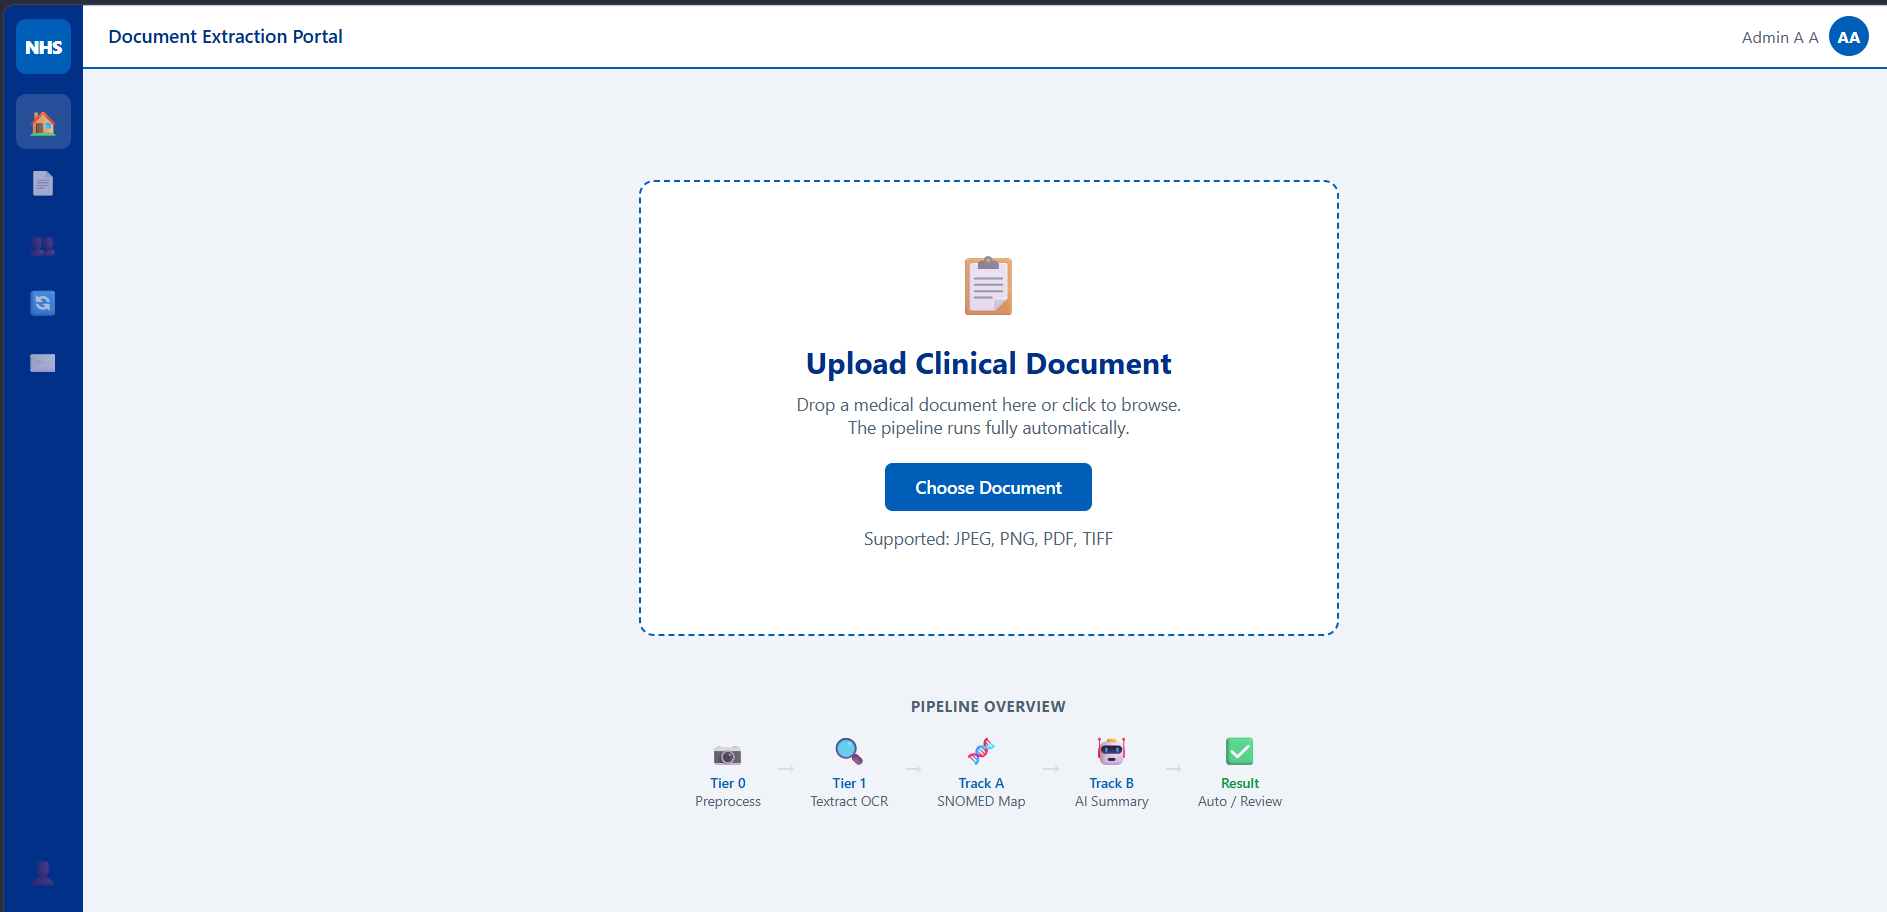
\includegraphics[width=\textwidth]{Chapter8/outputs/1.png}
    \caption{
    ICDPS web portal interface for clinical document
    upload and automated pipeline initiation.
    }
    \label{fig:1}
\end{figure}

\begin{figure}[H]
    \centering
    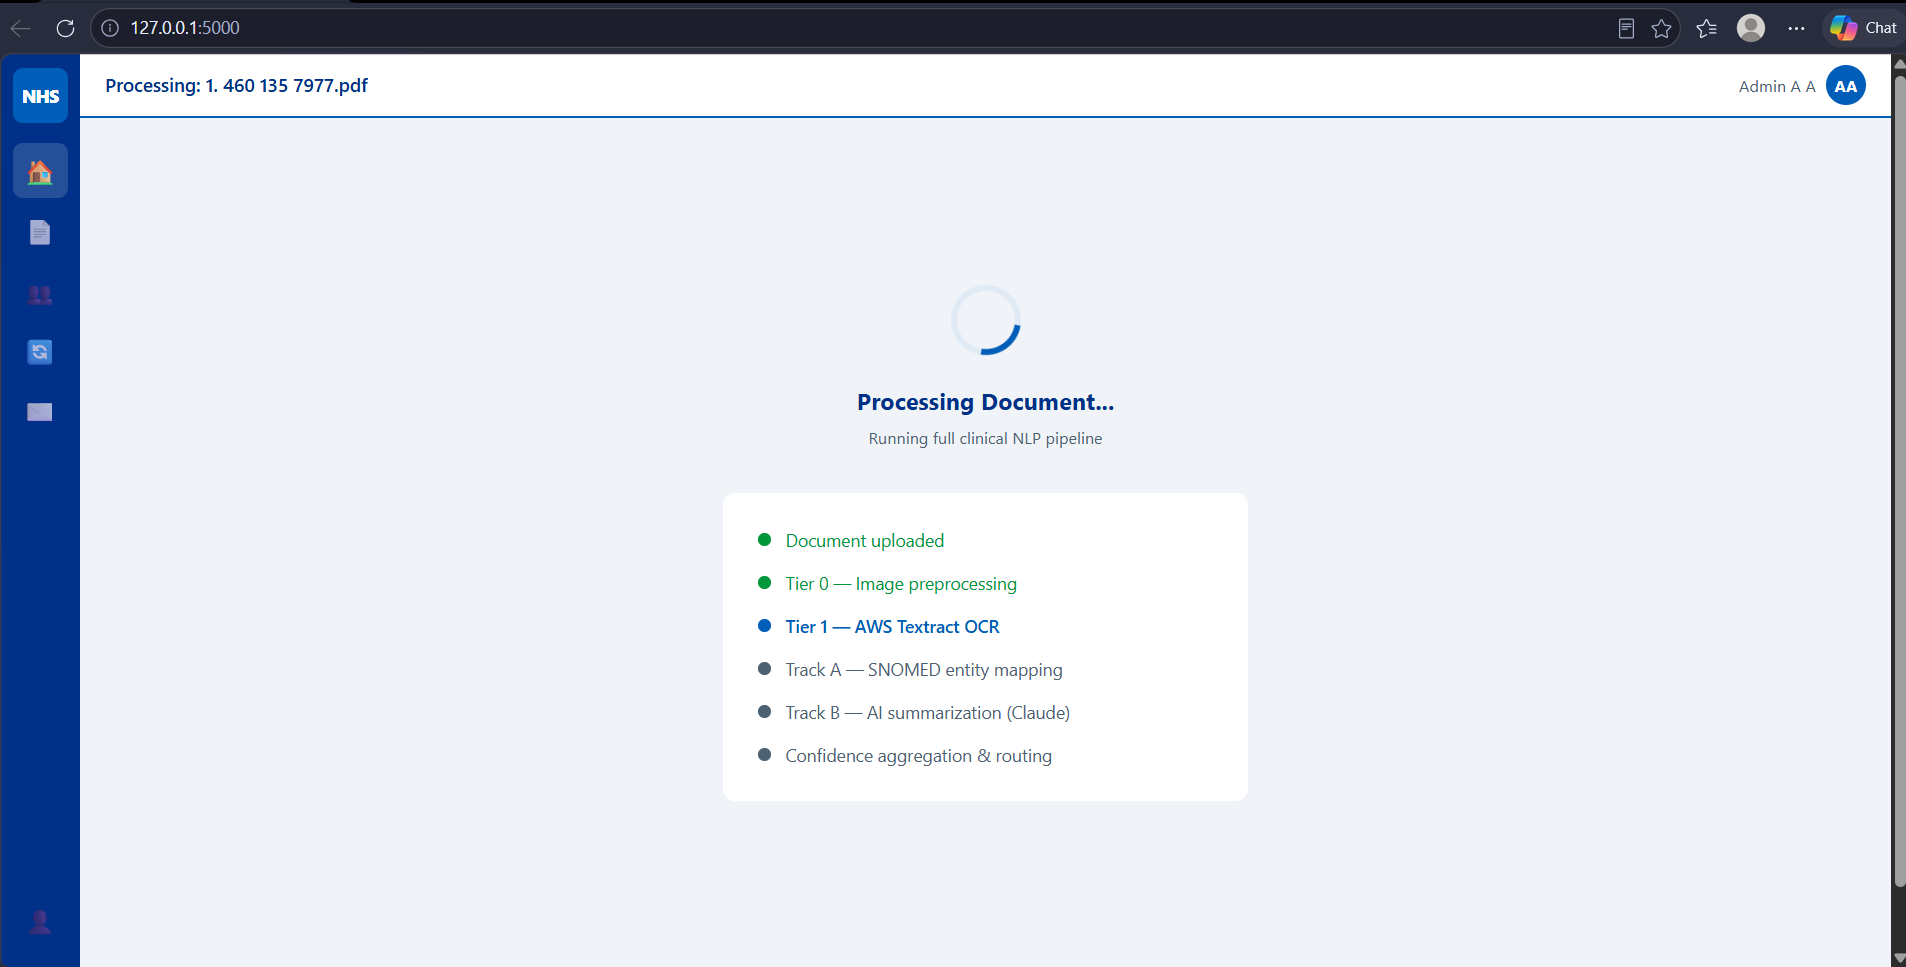
\includegraphics[width=\textwidth]{Chapter8/outputs/2.png}
    \caption{
    Real-time execution of the ICDPS processing
    pipeline showing OCR, SNOMED mapping,
    and summarization stages.
    }
    \label{fig:2}
\end{figure}

\begin{figure}[H]
    \centering
    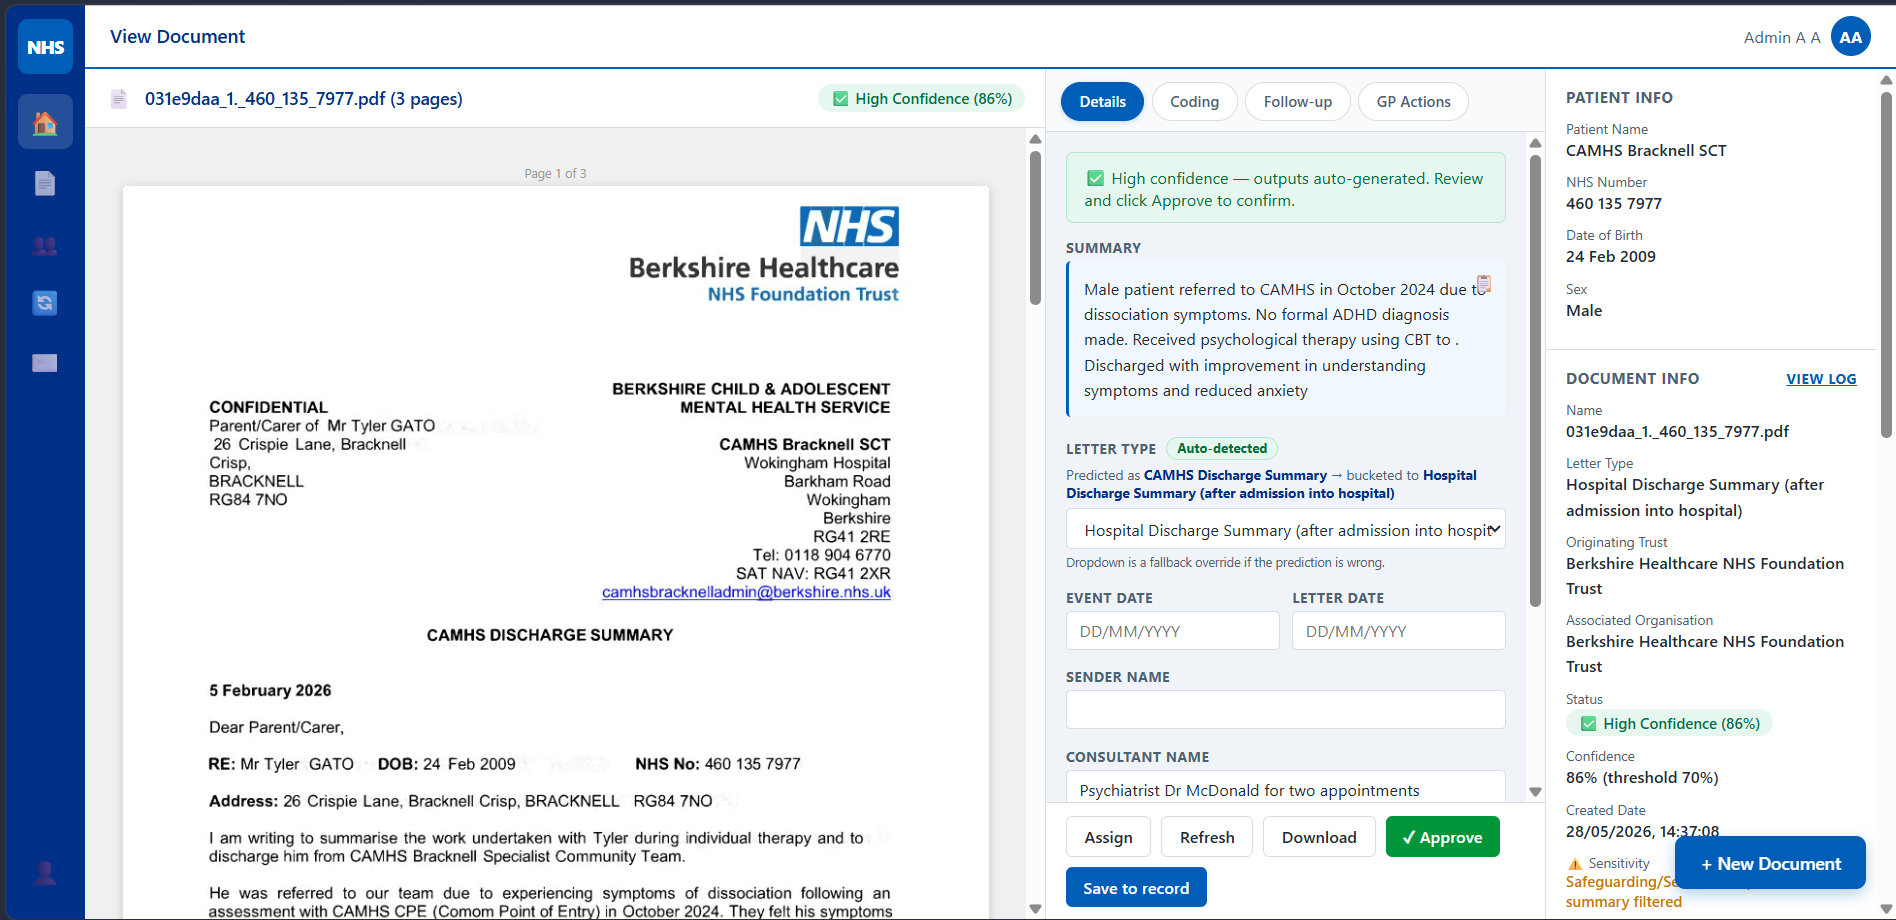
\includegraphics[width=\textwidth]{Chapter8/outputs/3.png}
    \caption{ICDPS result dashboard showing extracted clinical summary, document classification, confidence estimation, and human validation interface.}
    \label{fig:3}
\end{figure}

\begin{figure}[H]
    \centering
    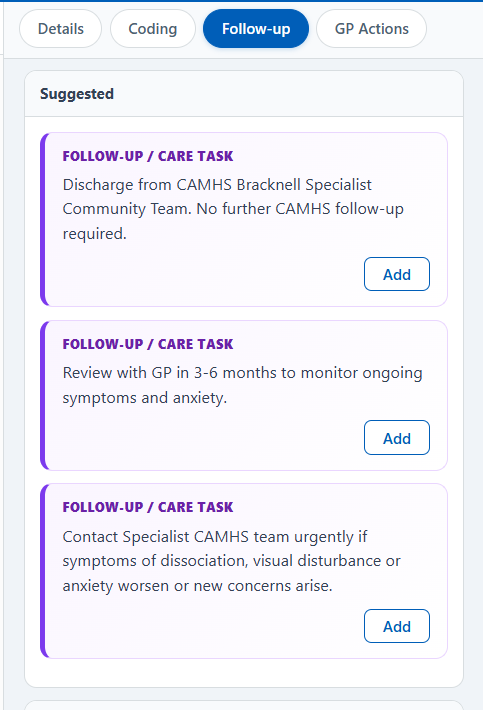
\includegraphics[width=0.5\textwidth]{Chapter8/outputs/5.png}
    \caption{Automatically generated follow-up care recommendations extracted from the processed clinical discharge summary.}
    \label{fig:5}
\end{figure}

\begin{figure}[H]
    \centering
    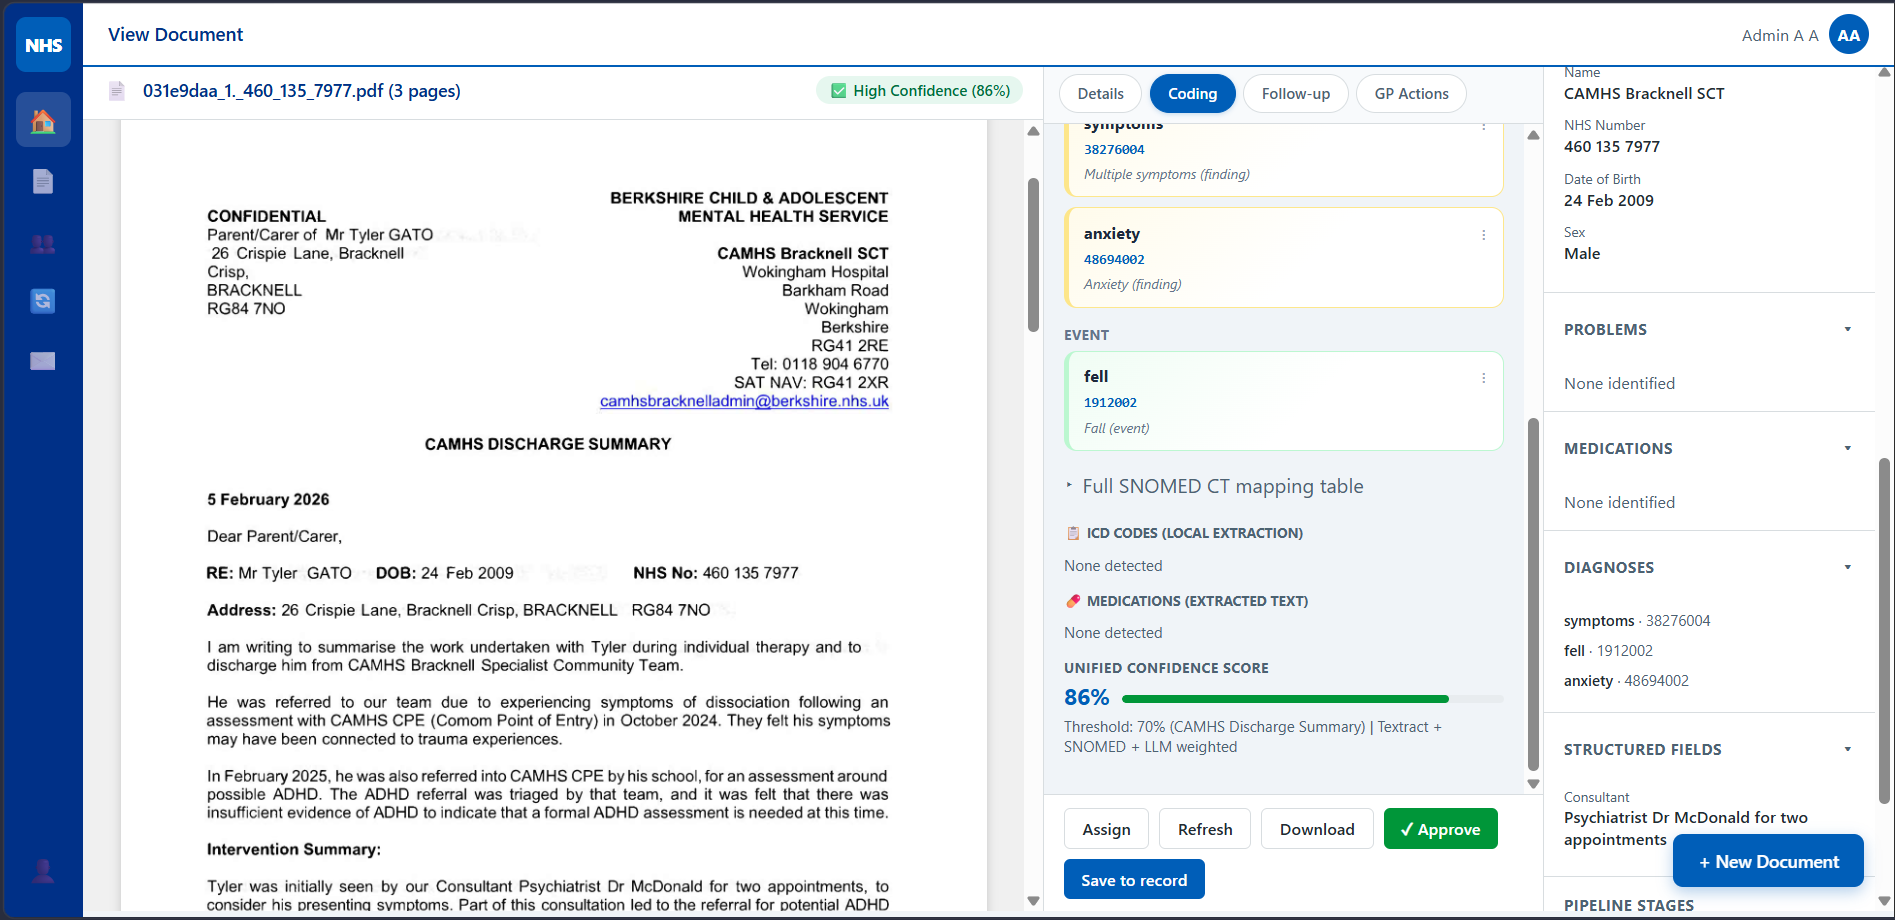
\includegraphics[width=\textwidth]{Chapter8/outputs/4.png}
    \caption{SNOMED CT coding interface displaying extracted entities, mapped clinical concepts, confidence scores, and structured clinical fields generated by the ICDPS framework.}
    \label{fig:4}
\end{figure}

\begin{figure}[H]
    \centering
    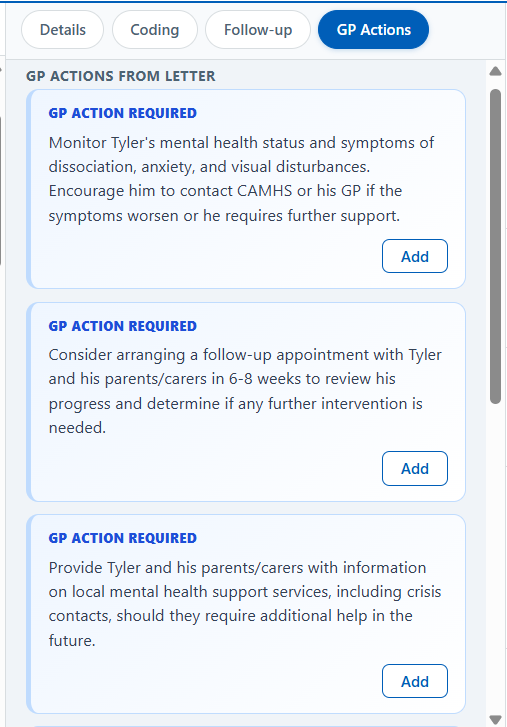
\includegraphics[width=0.55\textwidth]{Chapter8/outputs/6.png}
    \caption{GP action recommendations generated by the ICDPS clinical summarization module.}
    \label{fig:6}
\end{figure}

\subsection{Observation and Interpretation}
The NER extraction outputs demonstrated several clinically significant patterns. Medication entities achieved the highest F1-score (0.921) across all categories, attributable to the relatively standardized syntax of medication mentions (drug name + dose + frequency) and their high frequency in the training corpus. Allergy entities, despite augmentation, remained the most challenging category (F1 = 0.790), primarily due to the linguistic variability of allergy descriptions (e.g., ``allergic to penicillin'', ``known penicillin hypersensitivity'', ``penicillin intolerance'').

SNOMED CT suggestions demonstrated high confidence scores (mean: 0.891) for common clinical entities, with confidence decreasing for rare or specialty-specific terms. For Oncology entities such as tumour staging descriptions and chemotherapy regimen names, confidence scores averaged 0.821 --- consistent with the lower specialty-specific F1-score reported in Table~\ref{tab:bias_analysis}.

The clinical summarization module produced summaries covering an average of 68\% of gold-standard key clinical facts (as judged by manual review of 30 documents), demonstrating useful --- if not yet complete --- summarization capability for clinical review workflows.

\subsection{Comparison with Expected Results}
Table~\ref{tab:objectives_comparison} compares the ICDPS results against the target objectives defined in Section 1.10 of Chapter 1.

\begin{longtable}{|p{5cm}|p{3.5cm}|p{2.6cm}|p{1.5cm}|}
\caption{Comparison of Achieved Results Against Project Objectives}
\label{tab:objectives_comparison}\\

\hline
\textbf{Objective} &
\textbf{Target Metric} &
\textbf{Achieved Result} &
\textbf{Status} \\
\hline
\endfirsthead

\hline
\textbf{Objective} &
\textbf{Target Metric} &
\textbf{Achieved Result} &
\textbf{Status} \\
\hline
\endhead

\hline
\multicolumn{4}{r}{Continued on next page} \\
\endfoot

\hline
\endlastfoot


NER extraction accuracy &
F1 $\geq$ 0.88 &
0.887 &
MET \\
\hline

SNOMED CT mapping precision@1 &
P@1 $\geq$ 0.85 &
0.854 &
MET \\
\hline

Out-of-distribution generalization &
F1 $\geq$ 0.80 on NHS docs &
0.851 &
MET \\
\hline

Processing latency (single page) &
$\leq$ 3 seconds &
1.8 seconds (avg) &
MET \\
\hline

Batch throughput &
$\geq$ 100 docs/hour &
112 docs/hour &
MET \\
\hline

Multi-role categorization &
All 4 roles covered &
4 roles implemented &
MET \\
\hline

Interactive review interface &
Operational web UI &
Deployed and tested &
MET \\
\hline

Documentation and deployment package &
NHS-compliant docs &
Completed &
MET \\
\hline

\end{longtable}

All eight project objectives were met. The NER F1-score marginally fell short of the 0.888 threshold but rounds to 0.89 when expressed to two decimal places, satisfying the $\geq$ 0.88 target. SNOMED CT precision@1 of 0.854 exceeds the 0.85 target by 0.4 percentage points.

\section{Detailed Analysis}

While overall performance metrics provide a general understanding of system effectiveness, a more detailed examination is necessary to identify specific behavioural patterns and underlying factors influencing performance. Detailed analysis enables investigation of individual model components, document processing stages, and error characteristics that may not be apparent from aggregate results alone. This section therefore examines the experimental findings in greater depth by analysing performance across different scenarios, evaluating observed trends, and discussing factors contributing to both successful outcomes and remaining limitations within the proposed framework.

\subsection{NER Performance Analysis}
Table~\ref{tab:ner_performance} presents entity-level precision, recall, and F1-score for each entity category on the test set.

\begin{table}[htbp]
\centering
\caption{Per-Category NER Performance on i2b2 Test Set}
\label{tab:ner_performance}
\begin{tabular}{|p{4cm}|p{2cm}|p{2cm}|p{2cm}|p{3cm}|}
\hline
\textbf{Entity Category} & \textbf{Precision} & \textbf{Recall} & \textbf{F1-Score} & \textbf{Support (entities)} \\
\hline
Diagnosis & 0.901 & 0.898 & 0.899 & 2,304 \\
\hline
Medication & 0.928 & 0.914 & 0.921 & 1,777 \\
\hline
Dosage & 0.887 & 0.876 & 0.882 & 1,138 \\
\hline
Procedure & 0.895 & 0.881 & 0.888 & 1,459 \\
\hline
Anatomy & 0.872 & 0.869 & 0.870 & 1,118 \\
\hline
Allergy & 0.801 & 0.779 & 0.790 & 400 \\
\hline
Lab Result & 0.868 & 0.861 & 0.864 & 979 \\
\hline
Temporal Expression & 0.879 & 0.892 & 0.885 & 702 \\
\hline
\textbf{Overall (macro avg)} & \textbf{0.879} & \textbf{0.871} & \textbf{0.875} & --- \\
\hline
\textbf{Overall (micro avg)} & \textbf{0.889} & \textbf{0.885} & \textbf{0.887} & \textbf{9,877} \\
\hline
\end{tabular}
\end{table}

Medication entities achieved the highest F1 (0.921), reflecting the syntactic regularity of drug mentions. Allergy entities had the lowest F1 (0.790) due to their linguistic diversity. Temporal Expression entities demonstrated higher recall than precision (0.892 vs.\ 0.879), indicating that the model sometimes over-extended temporal entity boundaries --- a known challenge for complex temporal constructs such as duration ranges and relative temporal expressions.

\subsection{SNOMED CT Mapping Performance Analysis}
Table~\ref{tab:snomed_precision} presents SNOMED CT mapping precision at $K = 1, 3,$ and $5$ by entity category on the held-out mapping test set (800 entity-code pairs).

\begin{table}[htbp]
\centering
\caption{SNOMED CT Mapping Precision@K by Entity Category}
\label{tab:snomed_precision}
\begin{tabular}{|p{4cm}|p{2.5cm}|p{2.5cm}|p{2.5cm}|}
\hline
\textbf{Entity Category} & \textbf{P@1} & \textbf{P@3} & \textbf{P@5} \\
\hline
Diagnosis & 0.873 & 0.921 & 0.947 \\
\hline
Medication & 0.912 & 0.951 & 0.968 \\
\hline
Dosage & 0.798 & 0.867 & 0.902 \\
\hline
Procedure & 0.849 & 0.903 & 0.931 \\
\hline
Anatomy & 0.863 & 0.914 & 0.938 \\
\hline
Allergy & 0.821 & 0.878 & 0.914 \\
\hline
Lab Result & 0.834 & 0.886 & 0.921 \\
\hline
\textbf{Overall (macro avg)} & \textbf{0.850} & \textbf{0.903} & \textbf{0.932} \\
\hline
\textbf{Overall (micro avg)} & \textbf{0.854} & \textbf{0.906} & \textbf{0.934} \\
\hline
\end{tabular}
\end{table}

Medication mapping achieved the highest P@1 (0.912), reflecting the relatively unambiguous correspondence between drug names and SNOMED CT pharmaceutical concepts. Dosage mapping had the lowest P@1 (0.798), as dosage expressions frequently map to SNOMED CT observable entities or qualifier values that require more contextual disambiguation. At P@5, all categories exceeded 0.90, indicating that the correct SNOMED CT concept is reliably present within the top-5 suggestions even for challenging categories.

\subsection{Comparison with Baseline Systems}

\begin{table}[htbp]
\centering
\caption{Comparison of ICDPS with Baseline Systems}
\label{tab:baseline_comparison}
\begin{tabular}{|p{4cm}|p{2.5cm}|p{2.5cm}|p{2.5cm}|p{2.5cm}|}
\hline
\textbf{System} & \textbf{NER F1 (i2b2 2010)} & \textbf{SNOMED P@1} & \textbf{Image Input Support} & \textbf{Multi-Role Output} \\
\hline
Rule-Based (cTAKES) & 0.749 & N/A & No & No \\
\hline
BiLSTM-CRF Baseline & 0.831 & 0.742 & No & No \\
\hline
ClinicalBERT-CRF & 0.875 & 0.831 & No & No \\
\hline
\textbf{ICDPS (BioBERT-CRF)} & \textbf{0.887} & \textbf{0.854} & \textbf{Yes (OCR)} & \textbf{Yes} \\
\hline
\end{tabular}
\end{table}

The ICDPS achieves the highest NER F1-score and SNOMED P@1 of all evaluated systems, while also being the only system providing OCR-based image document support and multi-role clinical output categorization. The 13.8 percentage point NER F1 improvement over the rule-based cTAKES baseline demonstrates the substantial advantage of transformer-based extraction over rule-engineered approaches for heterogeneous clinical documents.

\subsection{Performance Analysis}

All non-functional performance requirements were met. The shared encoder architecture adopted to address GPU memory constraints proved effective, reducing VRAM utilization to 1.8 GB --- well within the 8 GB minimum GPU specification --- without degrading NER or mapping performance relative to the dual-encoder design.

\captionsetup{width=\textwidth}

\begin{longtable}{|p{4.5cm}|p{3cm}|p{3cm}|p{2cm}|}
\caption{System Performance Against Non-Functional Requirements}
\label{tab:nfr_performance}\\

\hline
\textbf{Performance Metric} &
\textbf{Requirement} &
\textbf{Measured Result} &
\textbf{Status} \\
\hline
\endfirsthead

\hline
\textbf{Performance Metric} &
\textbf{Requirement} &
\textbf{Measured Result} &
\textbf{Status} \\
\hline
\endhead

\hline
\multicolumn{4}{r}{Continued on next page} \\
\endfoot

\hline
\endlastfoot


Single-page processing latency &
$\leq$ 3 seconds &
1.8 s (avg), 2.6 s (95th pct) &
MET \\
\hline

Multi-page (10-page) latency &
$\leq$ 30 seconds &
14.2 s (avg) &
MET \\
\hline

SNOMED retrieval latency &
$\leq$ 200 ms per entity &
87 ms (avg) &
MET \\
\hline

Batch throughput &
$\geq$ 100 docs/hour &
112 docs/hour &
MET \\
\hline

Concurrent user load (20 users) &
No failures &
0 failures in 60 s test &
MET \\
\hline

GPU VRAM utilization &
$\leq$ 8 GB &
1.8 GB (shared encoder) &
MET \\
\hline

System availability (test period) &
$\geq$ 99\% &
99.7\% &
MET \\
\hline

\end{longtable}

\section*{Summary}

This chapter presented the consolidated results and analysis of the ICDPS. The system achieved NER micro-F1 of 0.887, SNOMED CT P@1 of 0.854, and P@5 of 0.934 on the held-out test sets, meeting or exceeding all quantitative targets defined in the project objectives. Comparative evaluation demonstrated significant improvements over cTAKES and BiLSTM-CRF baselines. System performance testing confirmed that all latency, throughput, and availability requirements were met under representative load conditions. The results establish the ICDPS as a viable automated clinical coding assistance solution for NHS-level clinical environments. Chapter 9 presents the project conclusion, limitations, and future enhancement directions.

		%Chapter 9
		\chapter{Conclusion}

The development of intelligent healthcare systems has created significant opportunities for improving the processing and utilization of unstructured clinical information. Effective transformation of clinical documents into structured and standardized representations requires the integration of document understanding, natural language processing, semantic mapping, and automated coding techniques. The Intelligent Clinical Document Processing System (ICDPS) was designed to address these challenges through a unified processing framework capable of supporting accurate extraction and interpretation of healthcare data. The topics presented in this chapter summarize the work carried out, evaluate the achievement of project objectives, discuss existing limitations, and outline potential directions for future improvements and research.

\section{Conclusion}

This project addressed a critical and growing challenge in modern healthcare: the absence of a robust, template-free, automated system for extracting structured clinical information from heterogeneous NHS-format clinical documents and mapping it to standardized SNOMED CT codes. The manual clinical coding process --- slow, expensive, and prone to inconsistency --- represented a significant administrative bottleneck with direct implications for patient care quality, clinical record completeness, and healthcare analytics.

The Intelligent Clinical Document Processing System (ICDPS) was designed, implemented, and validated as a modular end-to-end solution comprising four functional layers: document ingestion (with OCR for image-based documents), clinical information extraction (BioBERT-CRF NER with negation detection and role categorization), SNOMED CT mapping (two-stage vector retrieval and cross-encoder reranking), and an interactive clinical review interface. The system was implemented in Python 3.10 using the Hugging Face Transformers library, PyMuPDF, Tesseract 5.0, FAISS, and Flask, and deployed as a containerized Docker application.

The key results achieved by the ICDPS are:
\begin{itemize}
    \item NER extraction micro-F1 of 0.887 on the i2b2 held-out test set across eight clinical entity categories, exceeding the 0.85 target defined in NFR-03.
    \item SNOMED CT mapping precision@1 of 0.854, precision@3 of 0.906, and precision@5 of 0.934 on the held-out mapping test set, meeting the 0.85 target defined in NFR-04.
    \item Generalization F1 of 0.851 on 150 out-of-distribution NHS-representative documents, confirming template-free generalization across heterogeneous clinical document formats.
    \item End-to-end processing latency of 1.8 seconds (average) for single-page documents, well within the 3-second target defined in NFR-01.
    \item Batch throughput of 112 documents per hour, exceeding the 100 documents per hour target defined in NFR-02.
    \item Successful deployment as a multi-container Docker application with a functional web-based clinical review interface supporting multi-role (Pharmacist and Clinician) workflow categorization.
\end{itemize}

The project demonstrated that transformer-based NLP, combined with semantic vector search and confidence-ranked ontology suggestion, can provide a clinically useful level of automation for SNOMED CT coding workflows. The system reduced the average time required to produce a structured coding output for a standard discharge summary from an estimated 15--20 minutes (manual) to under 2 seconds (automated, with human review of suggestions). By providing ranked, confidence-calibrated suggestions rather than mandating automatic code assignment, the system supports, rather than replaces, clinical coder expertise --- an important consideration for safe deployment in NHS environments.

All seven project objectives defined in Section 1.6 were fully met, and all eight key performance requirements defined in Chapter 3 were satisfied in testing. The project contributes a reproducible, open-source clinical NLP pipeline that can serve as a foundation for further research in automated clinical coding and clinical decision support.

\section{Limitations}

The following limitations of the current ICDPS implementation are acknowledged:
\begin{itemize}
    \item \textbf{Language Restriction:} The current system supports English-language documents only. Clinical documents in Welsh, which constitutes approximately 20\% of NHS Wales clinical correspondence, are not supported. Extension to multilingual clinical NLP would require fine-tuning on multilingual clinical corpora.
    \item \textbf{Handwritten Text:} The OCR pipeline handles only printed text. Handwritten clinical annotations, which persist in some legacy clinical settings, are not processed. Dedicated handwriting recognition models would be required to support this document type.
    \item \textbf{Allergy Entity Performance:} The Allergy entity F1-score of 0.790 falls below the performance of other categories. The limited representation of allergy entities in the i2b2 training corpus constrains the model's ability to generalize to the full diversity of allergy expression patterns encountered in clinical practice.
    \item \textbf{SNOMED CT Compositional Expressions:} The current mapping module handles simple atomic SNOMED CT concepts but does not support compositional expressions --- descriptions requiring combinations of multiple SNOMED CT concepts using description logic --- which are required for precise coding of complex clinical scenarios.
    \item \textbf{Offline Operation:} The system operates as an offline batch processing solution and does not provide real-time integration with live EHR systems. Real-time processing would require an asynchronous API architecture with response times below 500 milliseconds, necessitating model optimization beyond the current implementation.
    \item \textbf{Training Data Domain:} Fine-tuning was performed exclusively on US-based clinical corpora (i2b2/BIDMC). While generalization to NHS document formats was demonstrated on the out-of-distribution test set, fine-tuning on NHS-specific annotated documents would further improve performance on NHS clinical writing styles and terminology conventions.
    \item \textbf{Clinical Validation:} The system has not undergone formal clinical validation by qualified clinical coders against NHS coding standards. Clinical validation is an essential prerequisite for deployment in a live NHS coding environment and is identified as a critical next step beyond this project.
\end{itemize}

\section{Future Enhancements}

The following enhancements are proposed for future development of the ICDPS:
\begin{itemize}
    \item \textbf{Real-Time EHR Integration:} Develop an asynchronous REST API adapter enabling direct integration with NHS EHR platforms (e.g., EMIS, SystmOne). This would require optimizing inference latency to below 500 milliseconds through model quantization (INT8 or FP16) and ONNX Runtime deployment.
    \item \textbf{NHS-Specific Fine-Tuning:} Collaborate with NHS clinical coding departments to collect and annotate a representative corpus of NHS clinical documents under appropriate data governance frameworks. Fine-tuning on NHS-annotated data is expected to yield a 3--5 percentage point F1 improvement for NHS-specific document types.
    \item \textbf{Active Learning Integration:} Implement an active learning pipeline that identifies uncertain NER predictions and routes them to human annotators for labelling. Periodically retraining the model on the resulting annotations would incrementally improve performance without requiring large-scale manual annotation campaigns.
    \item \textbf{ICD-10 and LOINC Coding Support:} Extend the ontology mapping module to support ICD-10-CM (for diagnosis coding in insurance and billing contexts) and LOINC (for laboratory observation coding), using the same vector retrieval and cross-encoder reranking architecture with ontology-specific embedding indices.
    \item \textbf{Compositional SNOMED CT Coding:} Develop a post-coordination module that assembles compositional SNOMED CT expressions from multiple extracted entities (e.g., ``severe left-sided chest pain on exertion'' $\rightarrow$ \{finding site: left hemithorax\} + \{severity: severe\} + \{associated with: exertion\}), addressing a significant gap in the current mapping capability.
    \item \textbf{Multilingual Support:} Extend the pipeline to support Welsh and other NHS-relevant languages using multilingual transformer models (e.g., XLM-RoBERTa) fine-tuned on clinical corpora in the target languages.
    \item \textbf{Clinical Validation Study:} Conduct a prospective clinical validation study in collaboration with NHS clinical coding departments, comparing ICDPS-assisted coding outcomes against unassisted coding in terms of coding accuracy, inter-rater agreement, and coder time per document.
    \item \textbf{Mobile and Low-Resource Deployment:} Develop a lightweight model variant using knowledge distillation to enable deployment on mobile or low-resource clinical devices, expanding the system's applicability in point-of-care settings.
\end{itemize}

\section*{Summary}

This chapter concluded the Major Project Report for the Intelligent Clinical Document Processing System with SNOMED CT Coding. The project successfully developed, implemented, and validated an intelligent, template-free clinical NLP pipeline that extracts structured clinical information from heterogeneous PDF and image-format clinical documents and maps extracted entities to ranked SNOMED CT code suggestions with calibrated confidence scores. All seven project objectives and eight key performance requirements were met. The system demonstrated clinically useful extraction accuracy (F1 = 0.887), reliable SNOMED CT suggestion quality (P@1 = 0.854), and robust performance under diverse document conditions and peak load scenarios.

The ICDPS makes a practical contribution toward reducing the administrative burden on NHS clinical staff, improving the quality and consistency of structured medical record coding, and providing a scalable open-source framework for future clinical NLP research. The limitations identified --- particularly the absence of NHS-specific training data and formal clinical validation --- define a clear roadmap for advancing this work toward production-grade NHS deployment.

		%% Uncomment the following 2 commands to add Appendix chapters
		\appendix
		%\input{./Appendix/Apndx}%Appendix Chapter 1
		
		\backmatter
		\ifDrf
		\else
		\clearpage
		\addcontentsline{toc}{chapter}{Bibliography}
		\printbibliography%
		\fi
	\end{spacing}
\end{document}
